\newpage
\chapter{Criteria \& Tools}
\label{CriteriaTools}

In this chapter, the criteria that will be used in trading off the concepts will be discussed. For this both qualitative and quantitative criteria are used and the weights are determined. After the description of these criteria in \autoref{sec:Criteria}, in \autoref{sec:Tools} the tools used to find the values for these criteria are described. Following this will be an overview of the integration of all the tools in \ref{sec:toolintegration} and a sensitivity analysis in section \ref{sec:sensitivityanalysis}. 



\section{Criteria}
\label{sec:Criteria}


%Should we separate between qualitative and quantitative criteria?

In order to choose a final concept to be developed further during the detailed design phase, a set of criteria used to compare the candidate concepts must be established. The criteria, along with the weights associated with each criterion heavily affect the concept that gets chosen in the trade-off. Given that the criteria will drive the solution, it is wise to recall the mission need statement of the project, such that the concept which boils down from the criteria chosen does indeed adhere to the original goal and scope of the project:

\begin{quote}
    "To provide a sustainable, socially acceptable and economically competitive solution to meet urban transport demands of 2050 due to increasing urbanisation, congestion and energy demands."
\end{quote}

From the Mission Need Statement (MNS) above it becomes clear that \textbf{sustainability}, \textbf{social acceptance} and \textbf{profitability} of the system should be the main drivers of the design. There are many ways that the system could be profitable, specifically, the system could target a large market share and make little profit per customer or target a small market share and make large profits per customer. Since the MNS also contains the need to solve congestion, the system designed in this project will target a large market share (the masses).

Each of the important aspects of the solution highlighted above can be assessed qualitatively and quantitatively (the distinction between qualitative and quantitative criteria is shown below). Aspects like profit are really hard to predict directly, so proxies (like trip time savings) have been compared instead. For the sake of reducing the criteria space, the total trip time savings per kilometer (time*pax/km) has been fixed across the different systems explored in the Mid-Term phase, which means it is excluded from the trade-off criteria. This also means that the proxy for revenue has been fixed and that comparing the cost of one system with the cost of another is similar to comparing the profit of the two.

\subsection{Ecological Sustainability}

\paragraph{Quantitative Criteria}

\begin{itemize}
    \item \underline{Energy demand/pax/km/day (PREE)}: This reflects the energy consumption of the system to be able to operate the vehicles for an entire day. It is normalized by passengers since a system that transports more passengers and consumes a proportionally higher amount of energy is not necessarily worse than a system which transports less passengers and consumes less amount of energy (the commuters that the latter system is not serving will have to be transported anyway). The energy is also normalized by kilometers since this allows us to compare how the different mobility systems perform with respect to existing transport modes. Energy usage will scale with travelled distance for all transport modes.  %Total energy consumption of the system is however a very important parameter to quantify the ecological sustainability of the system (and as will be seen later, it will also impact the cost of the system).
    \item \underline{Battery mass}: It is hard to foresee the development of battery chemistries up until 2050. As it stands today, however, batteries used in the car industry rely on rare Earth metals such as Lithium and Cobalt, which could become scarce by 2050 \footnote{\url{https://www.hannovermesse.de/en/news/raw-materials-for-lithium-ion-batteries-are-running-out-83008.xhtml} [accessed 15-05-2019]}. Batteries are also well known for being poorly recyclable, making it the least ecologically sustainable component in the vehicle. By multiplying the mass of batteries in each vehicle times the vehicles in the fleet, the total battery mass of the system can be calculated.
    
\end{itemize}

\subsection{Social acceptance}

\paragraph{Qualitative Criteria}

\begin{itemize}
    \item \underline{Safety}: Even though this is a qualitative criteria, it can be assessed by thinking about the number of fatalities per crash times the probability of a certain concept crashing. The number of fatalities per crash can be estimated by looking at the number of passengers and the crashworthiness of the vehicle (does it fall from the sky like a brick, does it autorotate, does it glide?). The probability of a crash can be estimated by looking for single points of failure in the concept or likely failure modes of the VTOL concept (Vortex Ring State for instance). Also a higher number of rotating elements gives a higher probability of failure than an aircraft that just uses control surfaces. 
    \item \underline{Passenger experience}: The passenger experience includes everything from comfort, view, motion sickness, luxury feeling, vibration levels, cabin noise, etc.
%    \item \underline{Urban disruption}:
\end{itemize}

\paragraph{Quantitative Criteria}

\begin{itemize}
    \item \underline{Downwash}: Downwash from the vehicle rotors is purely a result of thrust. However, the speed of this downwash heavily depends on the disk loading of the rotors, making it vehicle dependent. During take-off and landing operations, the downwash will impinge on the surface of the landing pad and could interfere with other vehicles and people in the surroundings. For decentralized landing pads, which could be placed at street level, the downwash could blow off dust and become annoying for people waiting to board or anyone in the near surroundings. 
    
    \item \underline{Noise}: When developing a UAM system, noise is one of the main concerns for the community. Aircraft and rotorcraft generally generate a lot of noise, which is disturbing for non-users, but also for the ride comfort a quiet vehicle would be more attractive. Next to the actual volume of the vehicle, also the frequency of the noise should be considered. As small rotors typically rotate with a higher frequency, this will create a higher pitch noise, which could cause more annoyance. 
    
    %item \underline{Congestion alleviation?}:
\end{itemize}




\subsection{Cost/Profit}

\paragraph{Qualitative Criteria}


\begin{itemize}
    \item \underline{Development costs}: Developments costs are harder to estimate numerically than operational and production costs. This is the reason why they have not been included in the MATLAB tool (so not included in the ticket price calculation). Development costs have instead been kept as an independent qualitative criterion. They will be estimated for each concept based on the technology readiness and the novelty of the concept which will directly translate to the analysis and testing efforts required to bring the concept to market.
\end{itemize}

\paragraph{Quantitative Criteria}



\begin{itemize}
    %\item \underline{Production costs}: This includes ...
   % \item \underline{Operational costs}: this includes
   \item \underline{Ticket price/pax/km}: This metric is found by calculating the production cost of the fleet of vehicles (cost of batteries, OEW, avionics) plus the cost of operating the fleet of vehicles (energy price, piloting, mechanics, groundcrew, and vertiport area fee) up to the BEP and divided by the number of revenue pax*km that the service will provide up to the BEP. 
\end{itemize}

\subsection{Technical Risk}

\paragraph{Qualitative Criteria}

\begin{itemize}
    \item \underline{ATM/UTM Efforts Needed}: This criterion analyses the level of complexity and the amount of effort needed to safely and efficiently organize and manage the system of vehicles in a city. The level of complexity is deduced by determining the level of interference with nearby airports, hospitals, military training grounds, drones, etc. Intersections of vehicle flight paths may occur, resulting in a more complex system,  as multiple intersections per fixed route may occur, possibly resulting in collision between two vehicles if the system is not well defined and managed. Apart from interference with other vehicles and areas, the positioning of landing sites are taken into account as well, as a 1-2 pax vehicle may easily land on top of a building, whereas a 20+ pax vehicle requires a properly designed vertiport.
    \item \underline{Susceptibility to weather conditions}: In this criterion the resistance of the vehicle to bad weather conditions like wind gusts during flight or crosswinds during vertical take-off and landing are analysed. Furthermore, the effects of air density and rain on the performance of the vehicle are analysed and taken into account as well. 
    \item \underline{Modification of current regulations}: This criterion takes the current FAA regulations into account. These regulations include those with respect to the airspace, various weight classes and regulation concerning autonomy of aircraft. 

  
\end{itemize}

%\paragraph{Quantitative Criteria}

%begin{itemize}
%   \item \underline{Pilot training hours}: number of vehicles
    
  
%\end{itemize}








%\begin{itemize}
    %\item \textbf{Maximum throughput}
    %\item \textbf{Sustainability} Energy per person per kilometer
    
    %\item \textbf{Social acceptance}
    
    %The social acceptance of the UAM system will be a function of two things. The first will be the noise that the system generates and the second will the downwash that is produced when the vehicle is in the vicinity of the landing site. For a first order estimation of the social acceptance of a solution it is assumed that both the noise and downwash are equally important to the level of social acceptance. 

    

    %\item \textbf{Cost/Profit}
    %\item \textbf{ATM/UTM efforts needed}
    
    %\item 
    
%    \item \textbf{Time gain versus existing transport modes}
%\end{itemize}


\subsection{Weights}
\label{subsec:weights}

As described in \autoref{comp}, the AHP method is used for the trade-off of the different concepts. For this an Excel sheet has been created where first the main criteria are scored on importance, followed by the sub-criteria. To find the final weights of the sub-criteria, their local weights are multiplied with the weights of the main criteria. To get an evenly matched weighting, all team members individually perform the pairwise comparisons of the criteria and these scores are combined. 



In \autoref{AHPtable} the weights of the criteria are shown. The individual weights resemble the weights of the sub-criteria compared to each other. These individual weights are then multiplied with the weights of the main criteria to find the total weight of each sub criterion.


\begin{table}[H]
\captionsetup{justification=centering}
\caption{Weightsof the criteria and sub-criteria}
\label{AHPtable}
\resizebox{\textwidth}{!}{%
\begin{tabular}{l|l|c|c}
\hline
\multicolumn{1}{c|}{\textbf{Criteria (weight)}}      & \multicolumn{1}{c|}{\textbf{Sub-criteria}} & \textbf{Individual weight}     & \textbf{Total weight}    \\ \hline
\multirow{2}{*}{\textbf{\begin{tabular}[l]{@{}l@{}}Ecological Sustainability\\ (0.36)\end{tabular}}} & Energy demand/hour                & 0.781                 & 0.278                 \\ \cline{2-4} 
                                                                                        & Battery mass  & 0.219                 & 0.078  \\ \hline
\multirow{4}{*}{\textbf{\begin{tabular}[l]{@{}l@{}}Social Acceptance \\ (0.31)\end{tabular}}} & Safety               & 0.593                      & 0.185                      \\ \cline{2-4} 
                                                                                       & Passenger experience & 0.179                      & 0.056                      \\ \cline{2-4} 
                                                                                       & Noise                & 0.176                      & 0.055                      \\ \cline{2-4} 
                                                                                       & Downwash             & 0.053 & 0.017 \\ \hline
\multirow{2}{*}{\textbf{\begin{tabular}[l]{@{}l@{}}Cost/Profit \\ (0.19)\end{tabular}}} & Development cost & 0.191                 & 0.036                 \\ \cline{2-4} 
                             & Ticket price  & 0.809                 & 0.153                               \\ \hline
\multirow{3}{*}{\textbf{\begin{tabular}[l]{@{}l@{}}Technical Risk\\ (0.14)\end{tabular}}} & ATM/UTM efforts                      & 0.569                 & 0.081                 \\ \cline{2-4} 
                                                                                          & Susceptibility to weather conditions & 0.304                 & 0.043                 \\ \cline{2-4} 
                                                                                          & Modification of regulations          & 0.127                 & 0.018                 \\ \hline
\end{tabular}%
}
\end{table}

To make sure no contradictions occur in scoring the criteria, a Consistency Ratio (CR) is computed. This number is a check that the different pairwise comparisons relate logical with each other and do not resemble a random distribution of the weights. The CR should have a value below $0.10$ for the weight determination to be considered acceptable \cite{AHPtut}. The CR values for this weighting determination where all found to be smaller than $0.10$, so the pairwise comparisons do not have to be revised.

\section{Tools}
\label{sec:Tools}

In order to get values for the different criteria and compare different concepts in a trade-off, tools are created. In this section all tools used for the determination of the values are described.

\subsection{Design Vector}
\label{subsec:desvector}
A numerical representation of the systems is the foundation of the tools outlined in this section, so its precise definition is given here to aid understanding the layout of the tools. An overview of the operational parameters is given in \autoref{OperationalIn}, with the atmospheric parameters in \autoref{AtmosphereIn}.

%\paragraph{Operational Parameters}

\begin{table}[]
\centering
\captionsetup{justification=centering}
\caption{Operational inputs}
\label{OperationalIn}
\begin{tabular}{|c|c|c|l|}
\Xhline{2\arrayrulewidth}
\multicolumn{1}{|l|}{} & \textbf{Parameter} & \textbf{Unit} & \textbf{Description} \\ \Xhline{2\arrayrulewidth}
\multirow{3}{*}{\rotatebox[origin=c]{90}{{\textbf{Fixed}}}} 
                       &    obj.S\_target     &    pax/m/s    &   Target system gain  \\ \cline{2-4} 
                       &    obj.cost.energy\_perkWh    &    USD/kWh    &   Energy cost per kWh (based on battery cost)  \\ \cline{2-4}
                       &    obj.cost.padfee\_perday     &    $USD/m^{2}/day$    &   Landing pad fee  \\ \cline{2-4}
                       &    obj.cost.BEP     &    years    &   Years until breakeven point  \\ \cline{2-4}
                       &    obj.pilots.rate     &    USD/hr    &   Pilot fee  \\ \cline{2-4}
                       &    obj.cost.grcrew\_perhour     &    USD/hr    &   Operations crew fee  \\ \cline{2-4}
                       &    obj.cost.mech\_perhour     &    USD/hr    &   Mechanics fee  \\ \cline{2-4}
                       &    obj.first\_last\_mile\_time     &    $s$    &   Time for first and last mile combined  \\ \cline{2-4}
                       &    obj.climb.initial\_lateral     &    m    &   Initial horizontal climb  \\ \cline{2-4}
                       &    obj.climb.initial\_vertical     &    m    &   Initial vertical climb  \\ \cline{2-4}
                       &    obj.taxi\_time    &    s    &   \begin{tabular}[c]{@{}l@{}}Land/take-off, taxi, de-spin/spin and standby\\ time\end{tabular}  \\ \cline{2-4}
                       &    obj.cost.dev     &    USD    &   Development cost for UAM  \\ \cline{2-4}
                       &    obj.TO\_TtoW\_ratio     &    -    &   Take-off thrust over weight ratio???  \\ \cline{2-4}
                       &    obj.climb.ROC     &    m/s    &   Rate of climb, climb phase  \\ \cline{2-4}
                       &    obj.cruise.alt     &    m    &   Cruise altitude  \\ \cline{2-4}
                       &    obj.hover.time     &    s    &   Hover time  \\ \cline{2-4}
                       &    obj.obs\_location.theta     &    rad    &   \begin{tabular}[c]{@{}l@{}}azimuth, RH positive top down, 0 through\\ nose\end{tabular}  \\ \cline{2-4}
                       &    obj.obs\_location.r     &    m    &   \begin{tabular}[c]{@{}l@{}}100 we are taking as the average skyscraper\\ height in downtown LA. So take-off in highly\\ populated areas will occur at 100 m altitude\end{tabular}  \\ \cline{2-4}
                       &    obj.cost.grcrew\_daily\_time     &    s/day/worker    &   Active working time ground crew  \\ \cline{2-4}
                       &    obj.cost.perhub     &    USD/hub    &   Cost to build a hub  \\ \cline{2-4}
                       &    obj.clearancegamma     &    rad    &   Clearance flight path angle  \\ \Xhline{2\arrayrulewidth}
\multirow{3}{*}{\rotatebox[origin=c]{90}{{\textbf{Variable}}}}  
                       &    obj.piloting     &    -    &   'piloted' or 'autonomous'  \\ \cline{2-4}
                       &    obj.min\_range     &    m    &   Minimum range  \\ \cline{2-4}
                       &    obj.cruise.vel     &    m/s    &   Cruise velocity  \\ \cline{2-4}
                       &    obj.climb.vclimb     &    m/s    &   Average velocity, climb phase  \\ \cline{2-4}
                       &    obj.climb.gamma     &    rad    &   Flight path angle, climb phase \\ \cline{2-4}
                       &    obj.pilots.num     &    -    &   Number of pilots per vehicle  \\ \cline{2-4}
                       &    obj.pilots.opsrate     &    -    &   \begin{tabular}[c]{@{}l@{}}Ratio pilot billed hours over flight operations\\ hours\end{tabular}   \\ \cline{2-4}
                       &    obj.cost.maint\_hours     &    -    &   Ratio maintenance hours over flight hours  \\ \cline{2-4}
                       &    obj.cost.grcrew\_num\_per\_pad     &    -    &   Number of ground crew workers per pad  \\ \cline{2-4}
                       &    obj.n     &    -    &   Number of routes to serve  \\ \Xhline{2\arrayrulewidth}
\end{tabular}
\end{table}

\begin{table}[]
\centering
\captionsetup{justification=centering}
\caption{Atmosphere inputs}
\label{AtmosphereIn}
\begin{tabular}{|c|c|c|l|}
\Xhline{2\arrayrulewidth}
\multicolumn{1}{|l|}{} & \textbf{Parameter} & \textbf{Unit} & \textbf{Description} \\ \Xhline{2\arrayrulewidth}
\multirow{3}{*}{\rotatebox[origin=c]{90}{{\textbf{Fixed}}}}  
                       &    obj.T     &    $K$    &   Local temperature  \\ \cline{2-4} 
                       &    obj.rho     &    $kg/m^{3}$    &   Local density  \\ \cline{2-4} 
                       &    obj.a     &    $m/s$    &   Speed of sound  \\ \cline{2-4}
                       &    obj.wind     &    $m/s$    &   Local wind speed  \\ \cline{2-4}
                       &    obj.rel\_humidity     &    \%    &   Local humidity  \\ \cline{2-4}
                       &    obj.p     &    $Pa$    &   Ambient pressure  \\ \Xhline{2\arrayrulewidth}
\end{tabular}
\end{table}

\vspace{-1mm}

\subsection{Vehicle Parameters}\label{stats}
Various tools require certain vehicle parameters as input, including the number of passengers, the cruise speed, the maximum range and energy used. In order to determine some realistic inputs, data has been collected from various sources on existing urban electric and hybrid aircraft currently in development.

\vspace{-4mm}

\begin{figure}[H]
\begin{subfigure}[t]{0.5\textwidth}
    \centering
    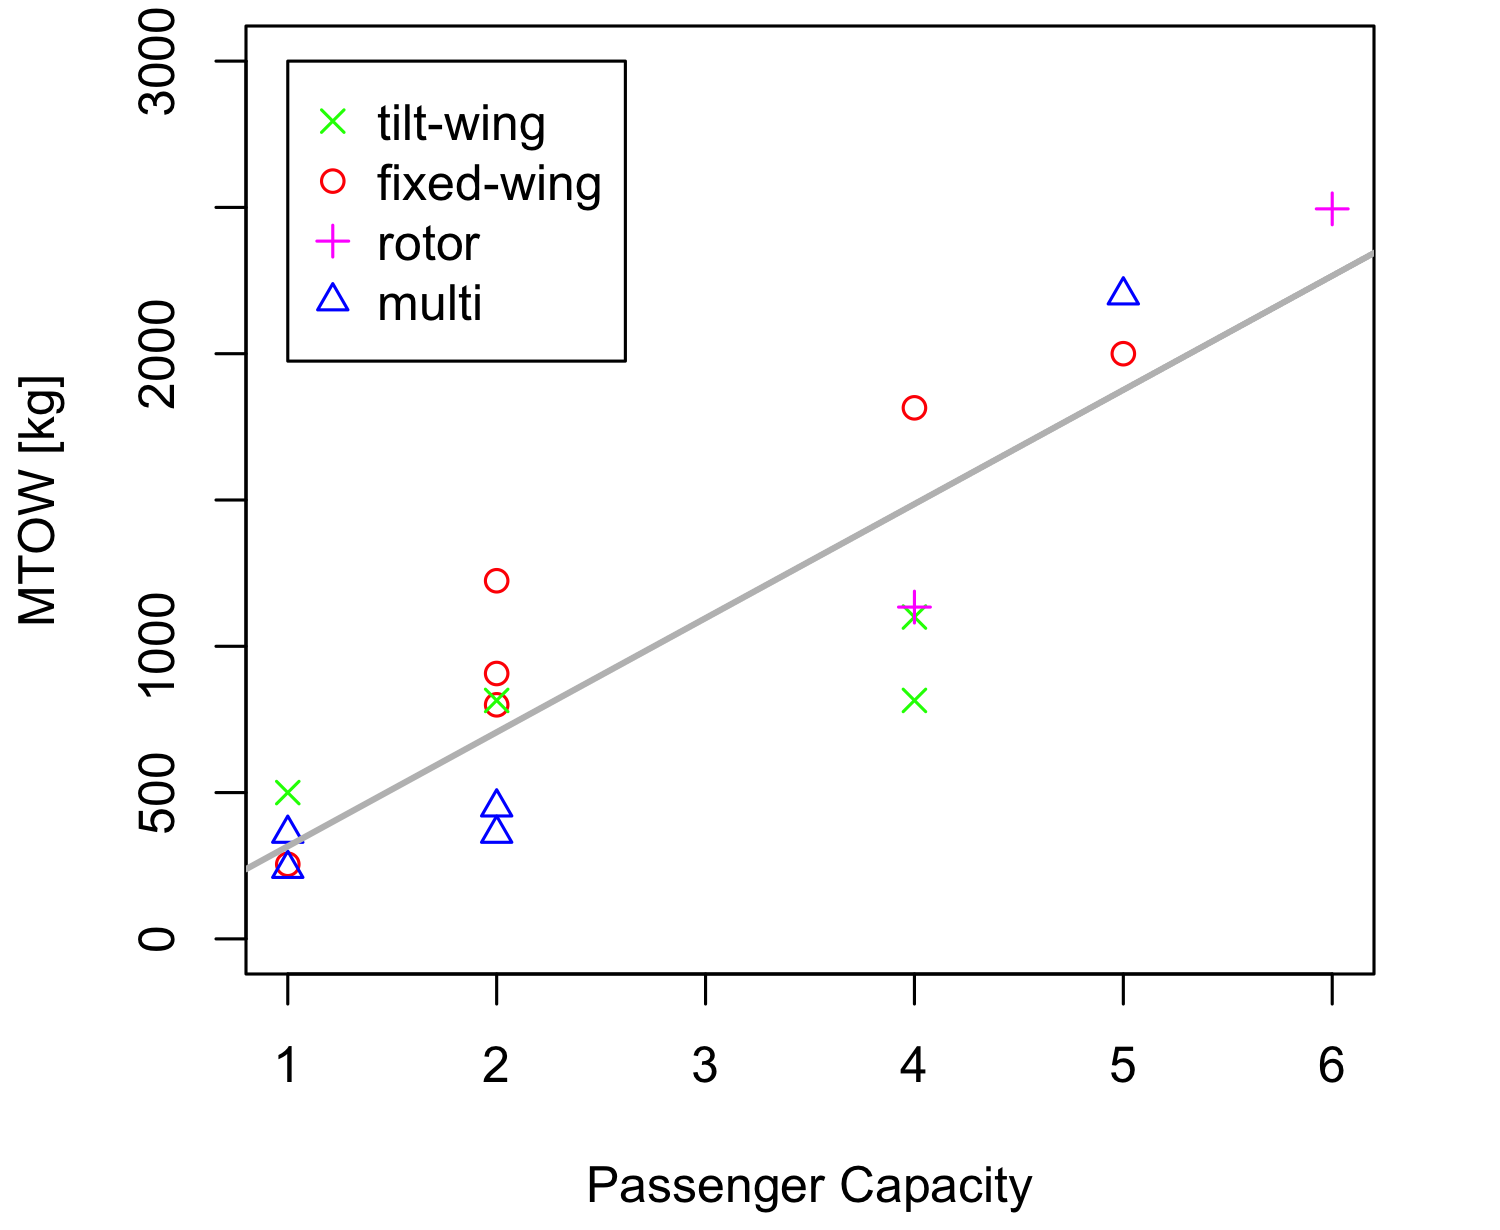
\includegraphics[width=\textwidth]{Figures/MTOW-Pax.png}
    \captionsetup{width=.8\linewidth}
    \caption{Linear regression fit of MTOW based on passenger capacity based on available concept specifications.}
    \label{fig:MTOW-Pax}
\end{subfigure}
\begin{subfigure}[t]{0.5\textwidth}
    \centering
    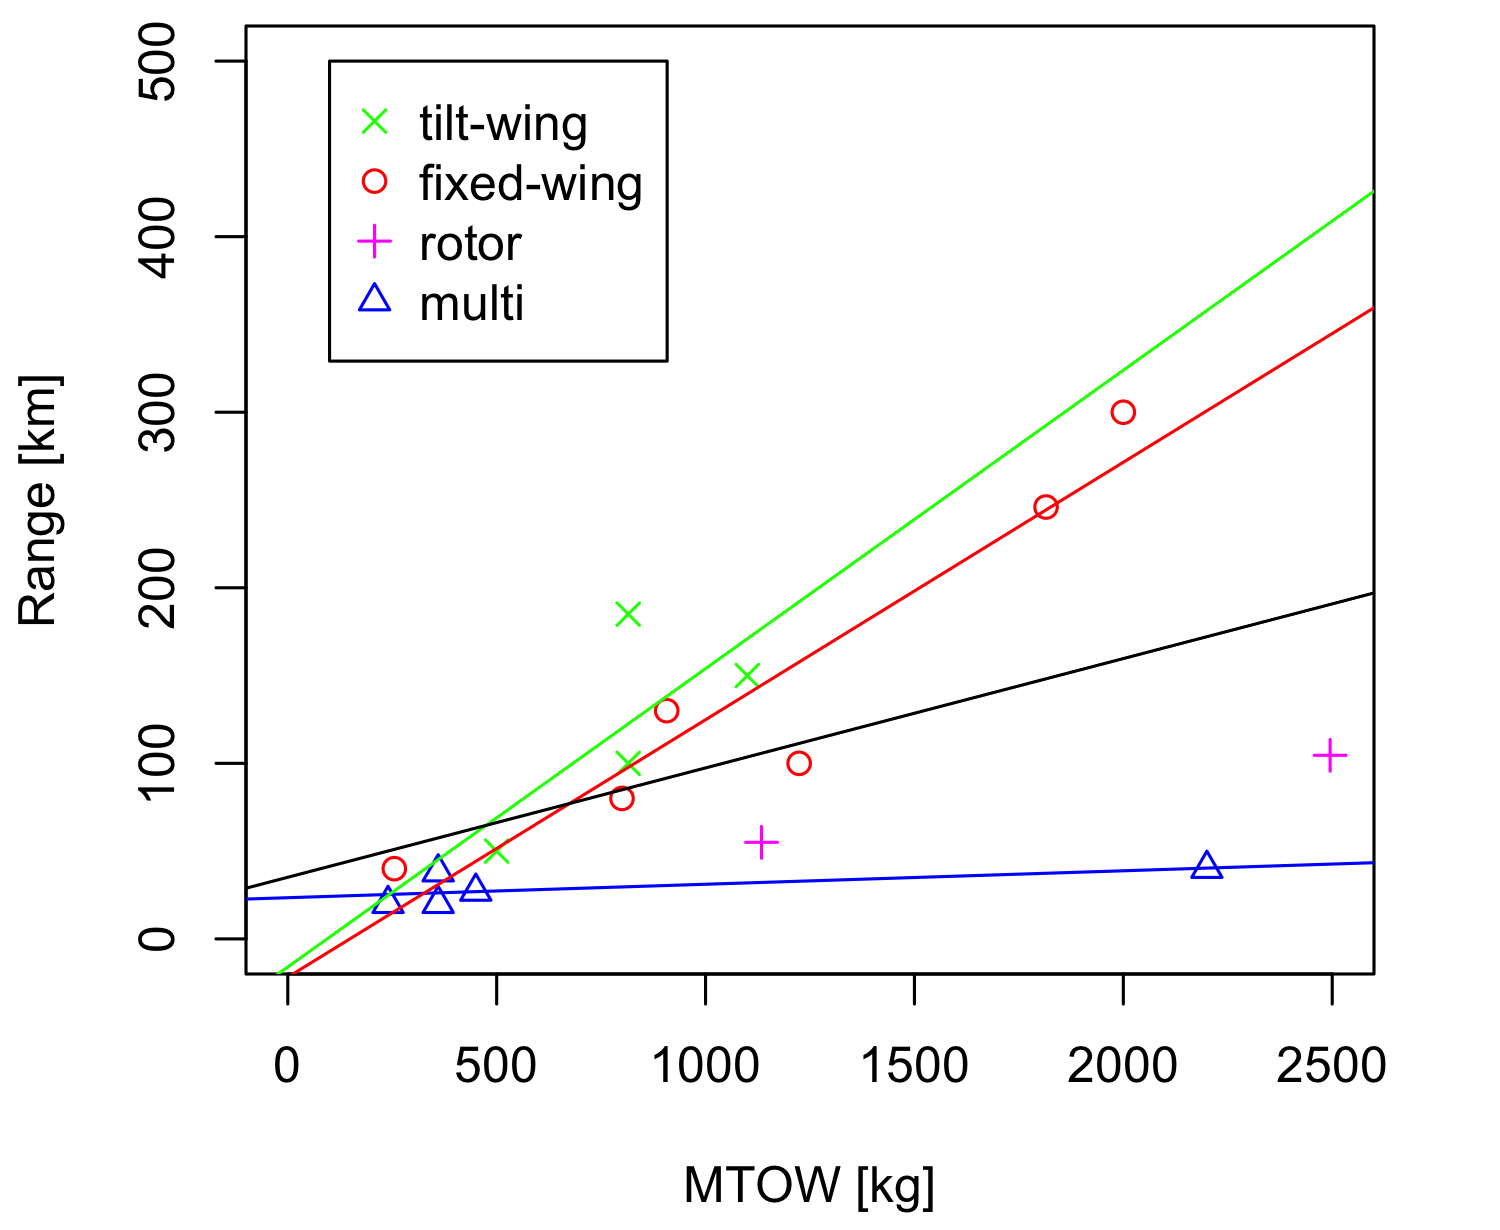
\includegraphics[width=\textwidth]{Figures/MTOW-Range.png}
    \captionsetup{width=.8\linewidth}
    \caption{Comparison of maximum range versus the MTOW of known electric eVTOL vehicles in development.}
    \label{fig:MTOW-Range}
\end{subfigure}
\captionsetup{justification=centering}
\caption{Verification of data accuracy}
\label{fig:MTOW-stats}
\end{figure}

Using statistical methods, some relationships can be derived from the data regarding MTOW, cruise speed and number of passengers. Since the aircraft differ quite a lot in configuration and level of development, the data points may not be entirely reliable, as performance may be overstated. However, as development and technology improve, it is likely that vehicles will even exceed this performance by 2050.

As shown in \autoref{fig:MTOW-Pax}, the MTOW increases with payload (passengers). The significance of this relation has a p-value of $6\cdot10^{-6}$ which is enough to reject the null hypothesis that there is no relationship (the data is available in \autoref{ap:eVTOL}). An analysis of variance (ANOVA) test regarding the co-variables of cruise speed, range and configuration show that the majority of the relation does come from the passenger capacity. For determining a realistic MTOW of each vehicle in the trade-off, the relation derived is a weight of 316 kg for a single passenger vehicle, and then 390 kg for each additional passenger.

There is also a clear difference depending on configuration. Specifically multi-copter and helicopter  arrangements require less mass, which is logical, as they have lower disk loading. This same relation extends to the cruise speed. While hover efficiency increases with decreasing disk loading, the cruise speed is also lower. In \autoref{fig:Cruise}, an average regression is given in black, as well as a fit for tilt-wing, fixed-wing and multi-rotorcraft. %Interestingly, the 4 passenger rotor point (pink plus), is a modified electric Robinson R44 helicopter\footnote{\url{http://evtol.news/aircraft/tier-1-robinson-r44/} [accessed on 15 May, 2019]}, which seems to fit with the multi-rotorcraft curve. 
The Carter Aviation Electric Air Taxi Concept\footnote{\url{http://www.cartercopters.com/pdfs/Carter_Electric_Air_Taxi.pdf} [accessed on 15 May, 2019]} (marked in \autoref{fig:Cruise-MTOW}), which features a rotor and a fixed-wing, thus it could fall into the fixed-wing category as well.

The relation between cruise and MTOW is also significant (p=0.0086), but is effected strongly by the configuration (p=0.00056). The relation of range to MTOW is also somewhat significant (p=0.025), where greater MTOW leads to greater range. The configuration has a large impact on the range as well (p=0.0196), as can be seen in \autoref{fig:MTOW-Range}. When comparing these electric aircraft to comparable hybrid or gasoline, the range is much lower. It is also impacted greatly by battery energy density. The effect of improved energy density is considered as technology is likely to improve by 2050.

\begin{figure}[H]
\captionsetup[subfigure]{justification=centering}
\begin{subfigure}[t]{0.5\textwidth}
    \centering
    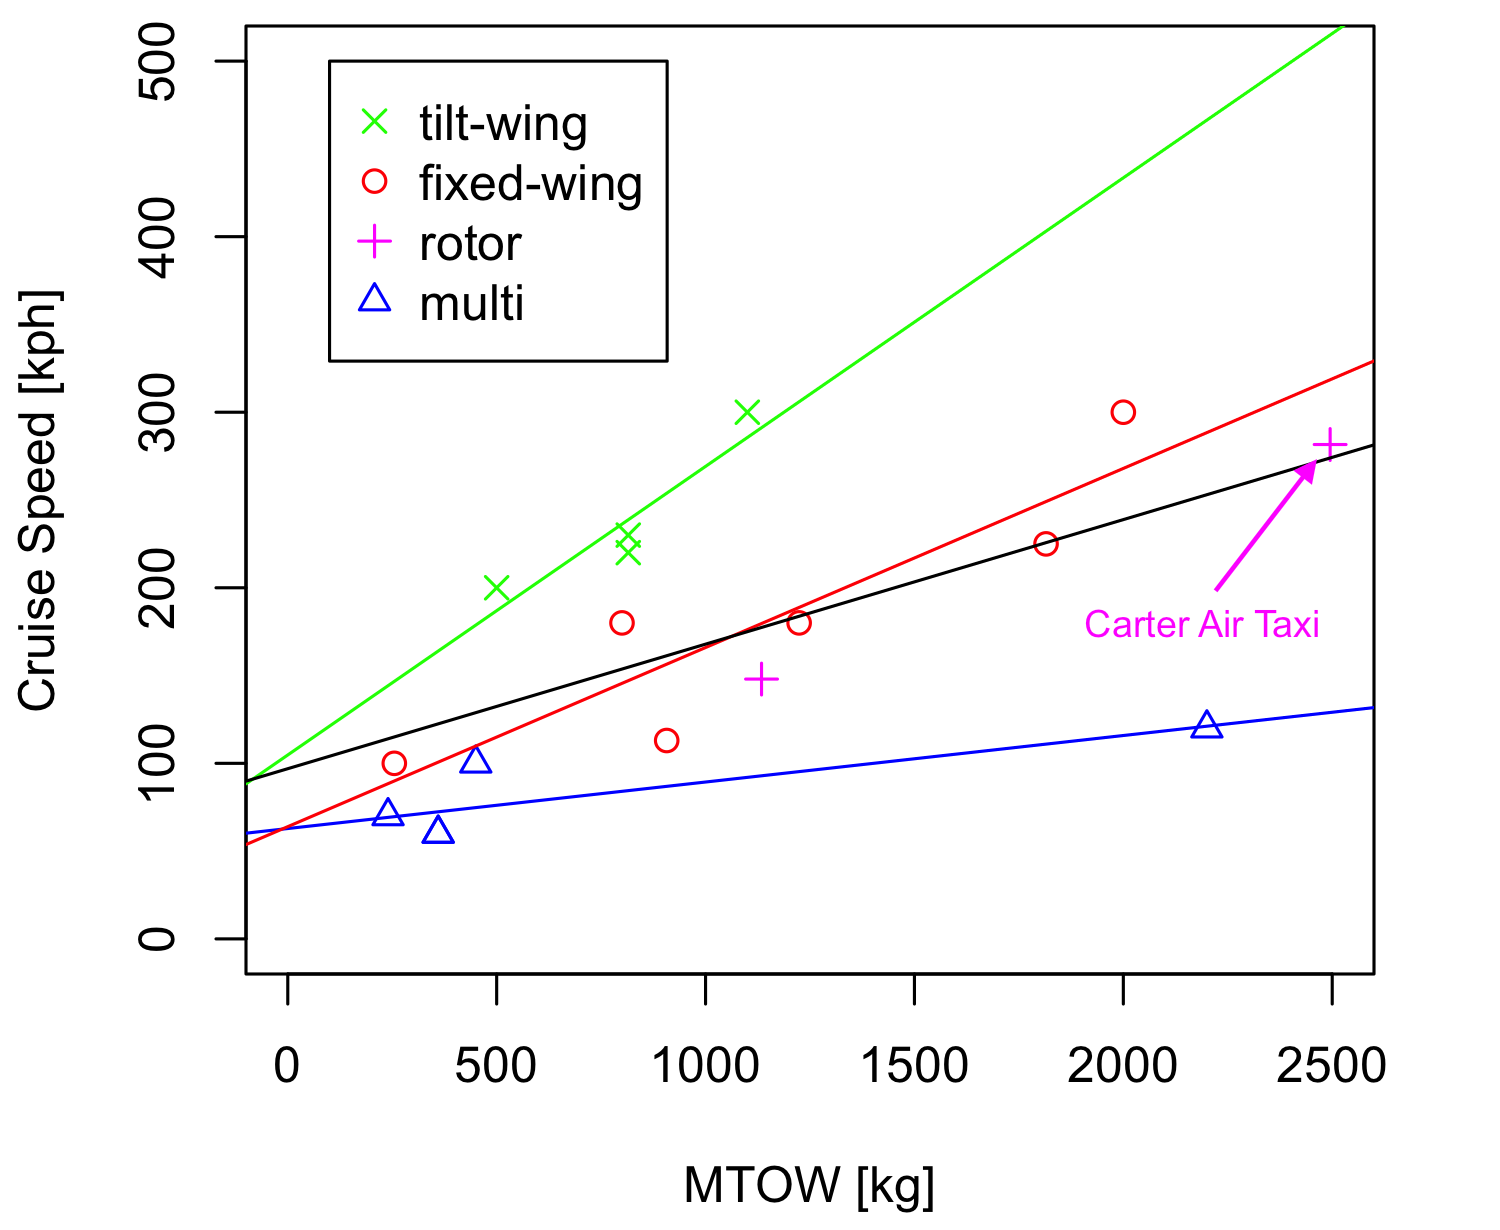
\includegraphics[width=\textwidth]{Figures/Cruise-MTOW.png}
    \caption{}
    \label{fig:Cruise-MTOW}
\end{subfigure}
\begin{subfigure}[t]{0.5\textwidth}
    \centering
    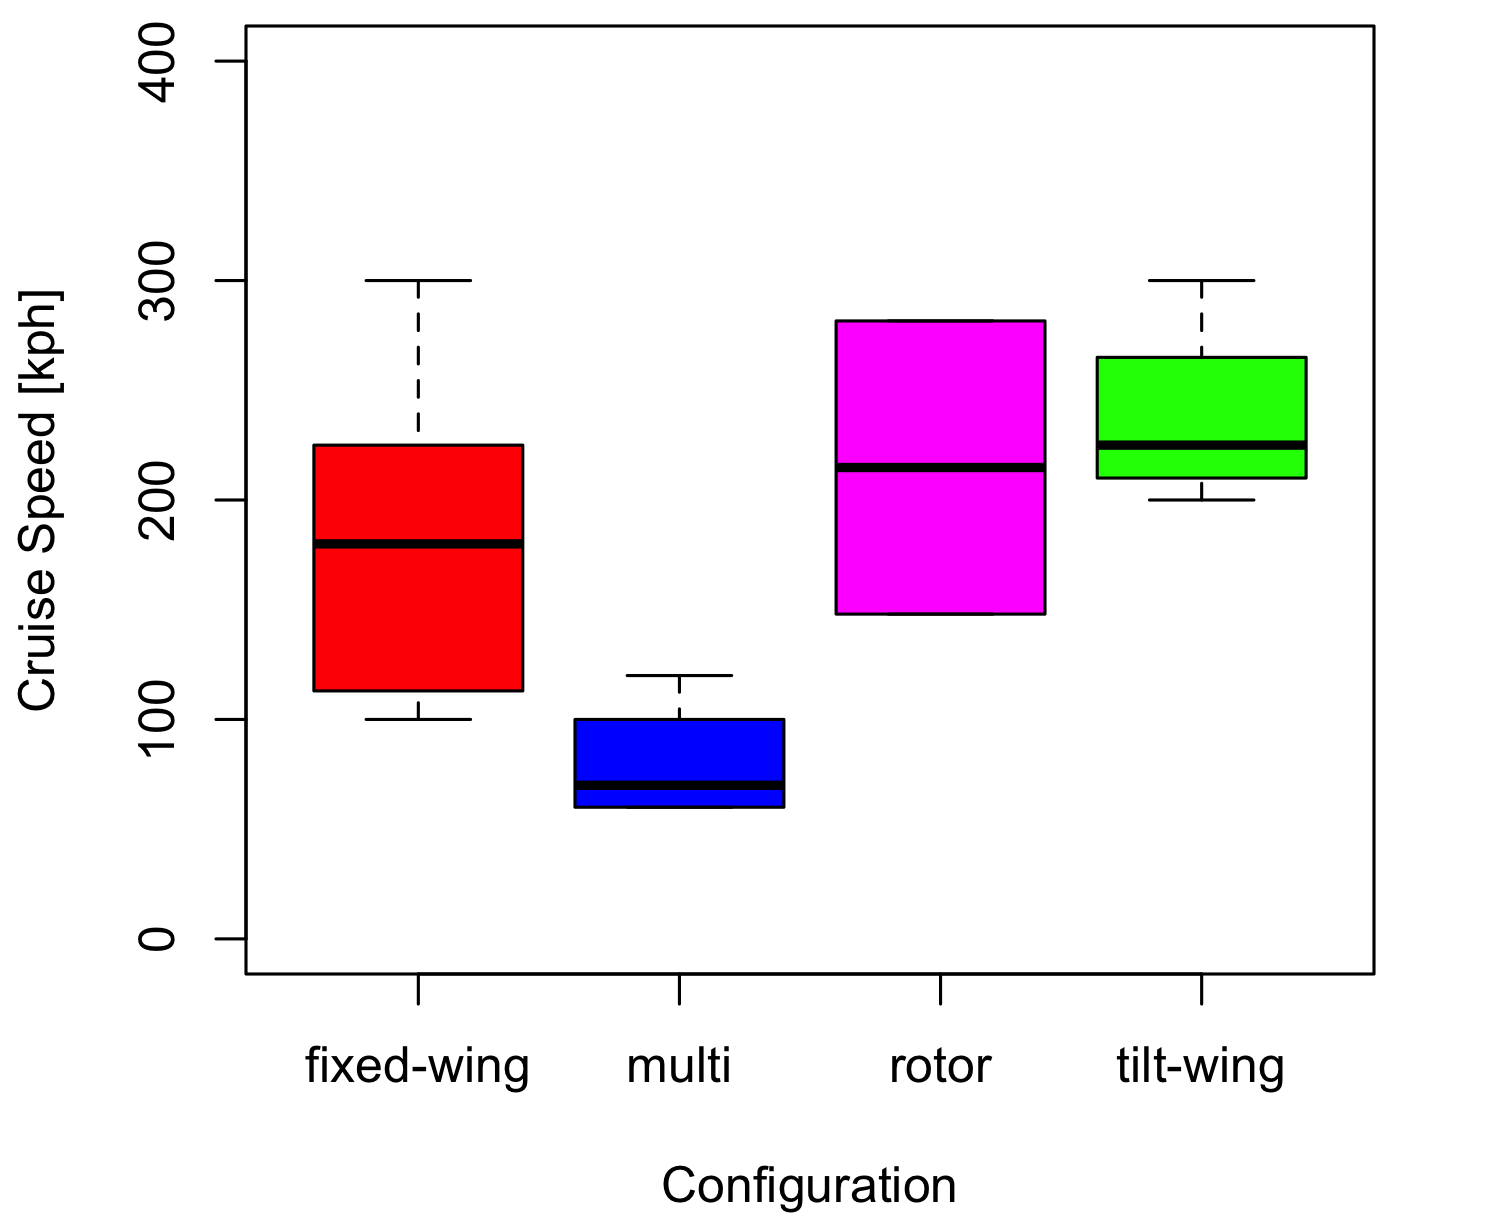
\includegraphics[width=\textwidth]{Figures/Cruise-config.png}
    \caption{}
    \label{fig:Cruise-config}
\end{subfigure}
    \captionsetup{justification=centering}
    \caption{Cruise speed is related to MTOW, but varies significantly with configuration.}
    \label{fig:Cruise}
\end{figure}

These relations allow the input parameters of range, cruise speed and passengers essentially become the requirements for the system selected via trade-off. So, if a short-range/slower vehicle is ideal for the system selected in trade-off (for example), then a multi-copter arrangement may be a good solution.

Since concepts that involve 20 passengers will also be considered, different relations will need to be used for those vehicles. No known eVTOL vehicles exist that carry more than 6 passengers. And, since the regressions used are linear, the relations begin to breakdown outside the range of known data points. For example, using these relations for a 20 passenger vehicle results in cruise speeds in excess of Mach 2.5. Naturally they should only be used for verification of designs carrying 6 or less passengers.

Instead, MTOW and cruise speeds are estimated from existing similar aircraft like the V-22 Osprey and Chinook helicopter. For range estimation, the energy methods proposed in \autoref{sec:energy} can be used.

\paragraph{Range and Power Consumption}\label{sec:energy}

To set an initial MTOW and range, existing vehicles are used as starting points. But in the trade-off, vehicles capable of different ranges must be considered. Existing studies show that in terms of energy consumption, urban air vehicles show the most efficiency gains over ground transport when the range is greater than 35 km \cite{ford}\cite{uberwhitepaper}. But the range for efficient travel must be compared to the demand for travel across certain ranges.

So, a method for interpolating vehicle characteristics with respect to required energy is used. By starting with known vehicle arrangements, the battery mass (including standardised margins) is calculated.

This is done using the energy assumptions given in \cite{ford}. The energy needed for a complete mission is determined from the power required for the three main flight phases: hover, climb/descent and cruise. \autoref{eq:power} and \autoref{eq:energy} are given in \cite{ford}. 

\begin{equation}
    \label{eq:power}
    \begin{split}
    P_\text{hover} &= \frac{mg}{\eta_h}\sqrt{\frac{\delta}{2\rho}}\\
    P_\text{climb} &= \frac{mg}{\eta_c}\left( \text{ROC} + \frac{V_\text{climb}}{L/D_\text{climb}} \right)\\
    P_\text{cruise} &= \frac{mg}{\frac{L}{D}}\frac{V_\text{cruise}}{\eta_c}
    \end{split}
\end{equation}

\begin{equation}
    \label{eq:energy}
    E = P_\text{hover}t_\text{hover} + P_\text{climb}t_\text{climb} + P_\text{cruise}t_\text{cruise}
\end{equation}

To make the best use of these relations, a flight profile must be defined. If a constant ROC is assumed, $V_\text{climb}$ may be different. Since the energy in climb is the power times the time, and if the the climb velocity is proportional to the cruise speed and ROC, the power in climb can be determined as a function of the cruise altitude, independent of time.

From the energy calculation, adjustments to the MTOW can be made when increasing or decreasing the range from a baseline vehicle design. By assuming a constant structural mass ratio ($1-\frac{m_\text{battery}+m_\text{payload}}{\text{MTOW}}$), a new required energy can be calculated for increased or decreased range requirement. Then, using a standard energy density for the new required battery mass, a new MTOW can be calculated. Naturally, this process must be iterated until it converges to a single solution for range, MTOW and battery mass. This method is useful if starting with an existing reference vehicle, but optimising for a shorter range.

This same energy calculation can also be used to determine the energy requirements during operations. For empty flights, substituting the OEW for MTOW will give the lower energy requirement. By assuming a "zombie" ratio of empty to full flights $c_\text{zombie}$, the total energy required for operations can be calculated, accounting for charge/discharge loss $\eta_\text{charge}$ as in \autoref{eq:energyTOTAL}.

\begin{equation}
    \label{eq:energyTOTAL}
    E_\text{day} = \eta_\text{zombie}\cdot N_\text{flights per day} \cdot \left[ E_\text{flight MTOW}c_\text{zombie} + E_\text{flight OEW}(1-c_\text{zombie}) \right]
\end{equation}

\begin{table}[H]
\centering
\captionsetup{justification=centering}
\caption{Vehicle inputs}
\label{VehicleIn}
\begin{tabular}{|c|c|c|l|}
\Xhline{2\arrayrulewidth}
\multicolumn{1}{|l|}{} & \textbf{Parameter} & \textbf{Unit} & \textbf{Description} \\ \Xhline{2\arrayrulewidth}
\multirow{3}{*}{\rotatebox[origin=c]{90}{{\textbf{Fixed}}}}  
                       &    obj.pax\_mass     &    kg    &   \begin{tabular}[c]{@{}l@{}}Passenger+payload mass (per\\ passenger)\end{tabular}  \\ \cline{2-4} 
                       &    obj.coax.trim     &    -    &   \begin{tabular}[c]{@{}l@{}}Coaxial rotor; ratio between lower rotor pitch\\ and upper rotor pitch\end{tabular}  \\ \cline{2-4}
                       &    obj.coax.kappaint     &    -    &   \begin{tabular}[c]{@{}l@{}}Coaxial rotor; induced power interference\\ factor\end{tabular}  \\ \cline{2-4}
                       &    obj.coax.rd     &    \%    &   Coaxial rotor; contraction radius  \\ \cline{2-4}
                       &    obj.cost.perkgmtow     &    USD    &   Vehicle cost per kg  \\ \cline{2-4}
                       &    obj.cost.avionics     &    USD    &   Avionics cost  \\ \cline{2-4}
                       &    obj.perf.nc     &    -    &   Cruise efficiency  \\ \cline{2-4}
                       &    obj.perf.nh     &    -    &   Hover efficiency  \\ \cline{2-4}
                       &    obj.perf.LoDclimb     &    -    &   Lift over drag - Climb  \\ \cline{2-4}
                       &    obj.bat.max\_ops\_charge     &    -    &   Maximum charge level during operations  \\ \cline{2-4}
                       &    obj.bat.min\_ops\_charge     &    -    &   Minimum charge level during operations  \\ \cline{2-4} 
                       &    modelpropunit.axialvel     &    m/s    &   Rotor axial velocity  \\ \cline{2-4}
                       &    modelrotor(1).solidity     &    -    &   Rotor blade solidity  \\ \cline{2-4}
                       &    modelrotor(1).kappa     &    -    &   single rotor induced power factor (Leishman)  \\ \cline{2-4}
                       &    modelrotor(1).blades.cl\_alpha     &    /\degree    &   Lift curve slope  \\ \cline{2-4}
                       &    modelrotor(1).blades.Cd0     &    -    &   Rotor blade profile drag  \\ \cline{2-4}
                       &    modelrotor(1).blades.D1     &    -    &   Quadratic coefficient drag curve  \\ \cline{2-4}
                       &    modelrotor(1).blades.D2     &   -    &   Linear coefficient drag curve  \\ \cline{2-4}
                       &    modelrotor(1).blades.pitch\_deg     &    \degree    &   Rotor blade pitch  \\ \Xhline{2\arrayrulewidth}
\multirow{3}{*}{\rotatebox[origin=c]{90}{{\textbf{Variable}}}}  
                       &    obj.max\_dim     &    m    &   Vehicle maximum dimension (any direction) \\ \cline{2-4}
                       &    obj.pax     &    people    &   Pax capacity vehicle \\ \cline{2-4}
                       &    obj.config     &    -    &   \begin{tabular}[c]{@{}l@{}}Vehicle configuration (outlier/tilt/fixed/multi\\/average)\end{tabular}  \\ \cline{2-4}
                       &    obj.struc.percent     &    \%    &   Vehicle structural percentage  \\ \cline{2-4}
                       &    obj.bat.P\_dens     &    W/kg    &   Battery power density  \\ \cline{2-4}
                       &    obj.bat.E\_dens     &    Wh/kg    &   Battery energy density  \\ \cline{2-4}
                       &    obj.bat.eta\_charge\_discharge     &    \%    &   Battery charge/discharge efficiency  \\ \cline{2-4}
                       &    obj.cost.bat\_perkWh     &    USD/kWh    &   Battery cost per kWh  \\ \cline{2-4}
                       &    obj.perf.maxrange     &    m    &   Vehicle maximum range  \\ \cline{2-4}
                       &    obj.perf.LoDcruise     &    -    &   Lift over drag, Cruise  \\ \cline{2-4}
                       &    modelpropunit.num     &    -    &   Number of units in a propulsion unit  \\ \cline{2-4}
                       &    modelpropunit.usage     &    -    &   Propulsion unit usage  \\ \cline{2-4}
                       &    modelpropunit.config     &    -    &   Rotor configuration in propulsion unit  \\ \cline{2-4}
                       &    modelpropunit.T\_percent\_hov     &    \%    &   \begin{tabular}[c]{@{}l@{}}Percentage of hover taken up by a propulsion\\ unit\end{tabular}  \\ \cline{2-4}
                       &    modelrotor(1).blades.num     &    -    &   Number of blades per rotor  \\ \cline{2-4}
                       &    modelrotor(1).radius     &    m    &   Rotor radius  \\ \cline{2-4}
                       &    modelrotor(1).omega     &    rad/s    &   Rotor radial velocity  \\ \Xhline{2\arrayrulewidth}
\end{tabular}
\end{table}

\subsection{Blade Element \& Momentum Theory (BEMT)}

A BEMT tool was developed for rotor performance calculations. In the current tool, the BEMT code is used as a way of calculating the rotational speed of a rotor (with fixed solidity and blade pitch angle) and the torque it generates for a given value of thrust required. This method is, however, much more versatile and it can be used in later stages of the design for rotor optimization (finding ideal airfoil, twist distribution, number of blades, chord, etc). The implementation of this BEMT tool is based on \cite{BEMT}, which describes a modelling approach for coaxial rotors in axial flight and hover. The approach is robust to single rotors as well, importantly.

BEMT is a standard method for the analysis of helicopter rotors, it was formalized for coaxial rotors by Leishman in \cite{BEMT}. The advantage of BEMT is that it is based on solid physical principles (mass, momentum and energy conservation laws) and is relatively free of empirical parameters. The theory discretizes the rotor disk into rotor annuli and applies momentum theory to each.

The main assumption of BEMT is that successive blade elements have no mutual effects on each other,(a two-dimensional assumption). Classic Prandtl “tip loss” effects have been included into the BEMT, giving a first approximation of the three-dimensional effects that occur due to tip and root vortices.


\begin{figure}[H]
\captionsetup[subfigure]{justification=centering}
\begin{subfigure}[t]{0.5\textwidth}
    \centering
    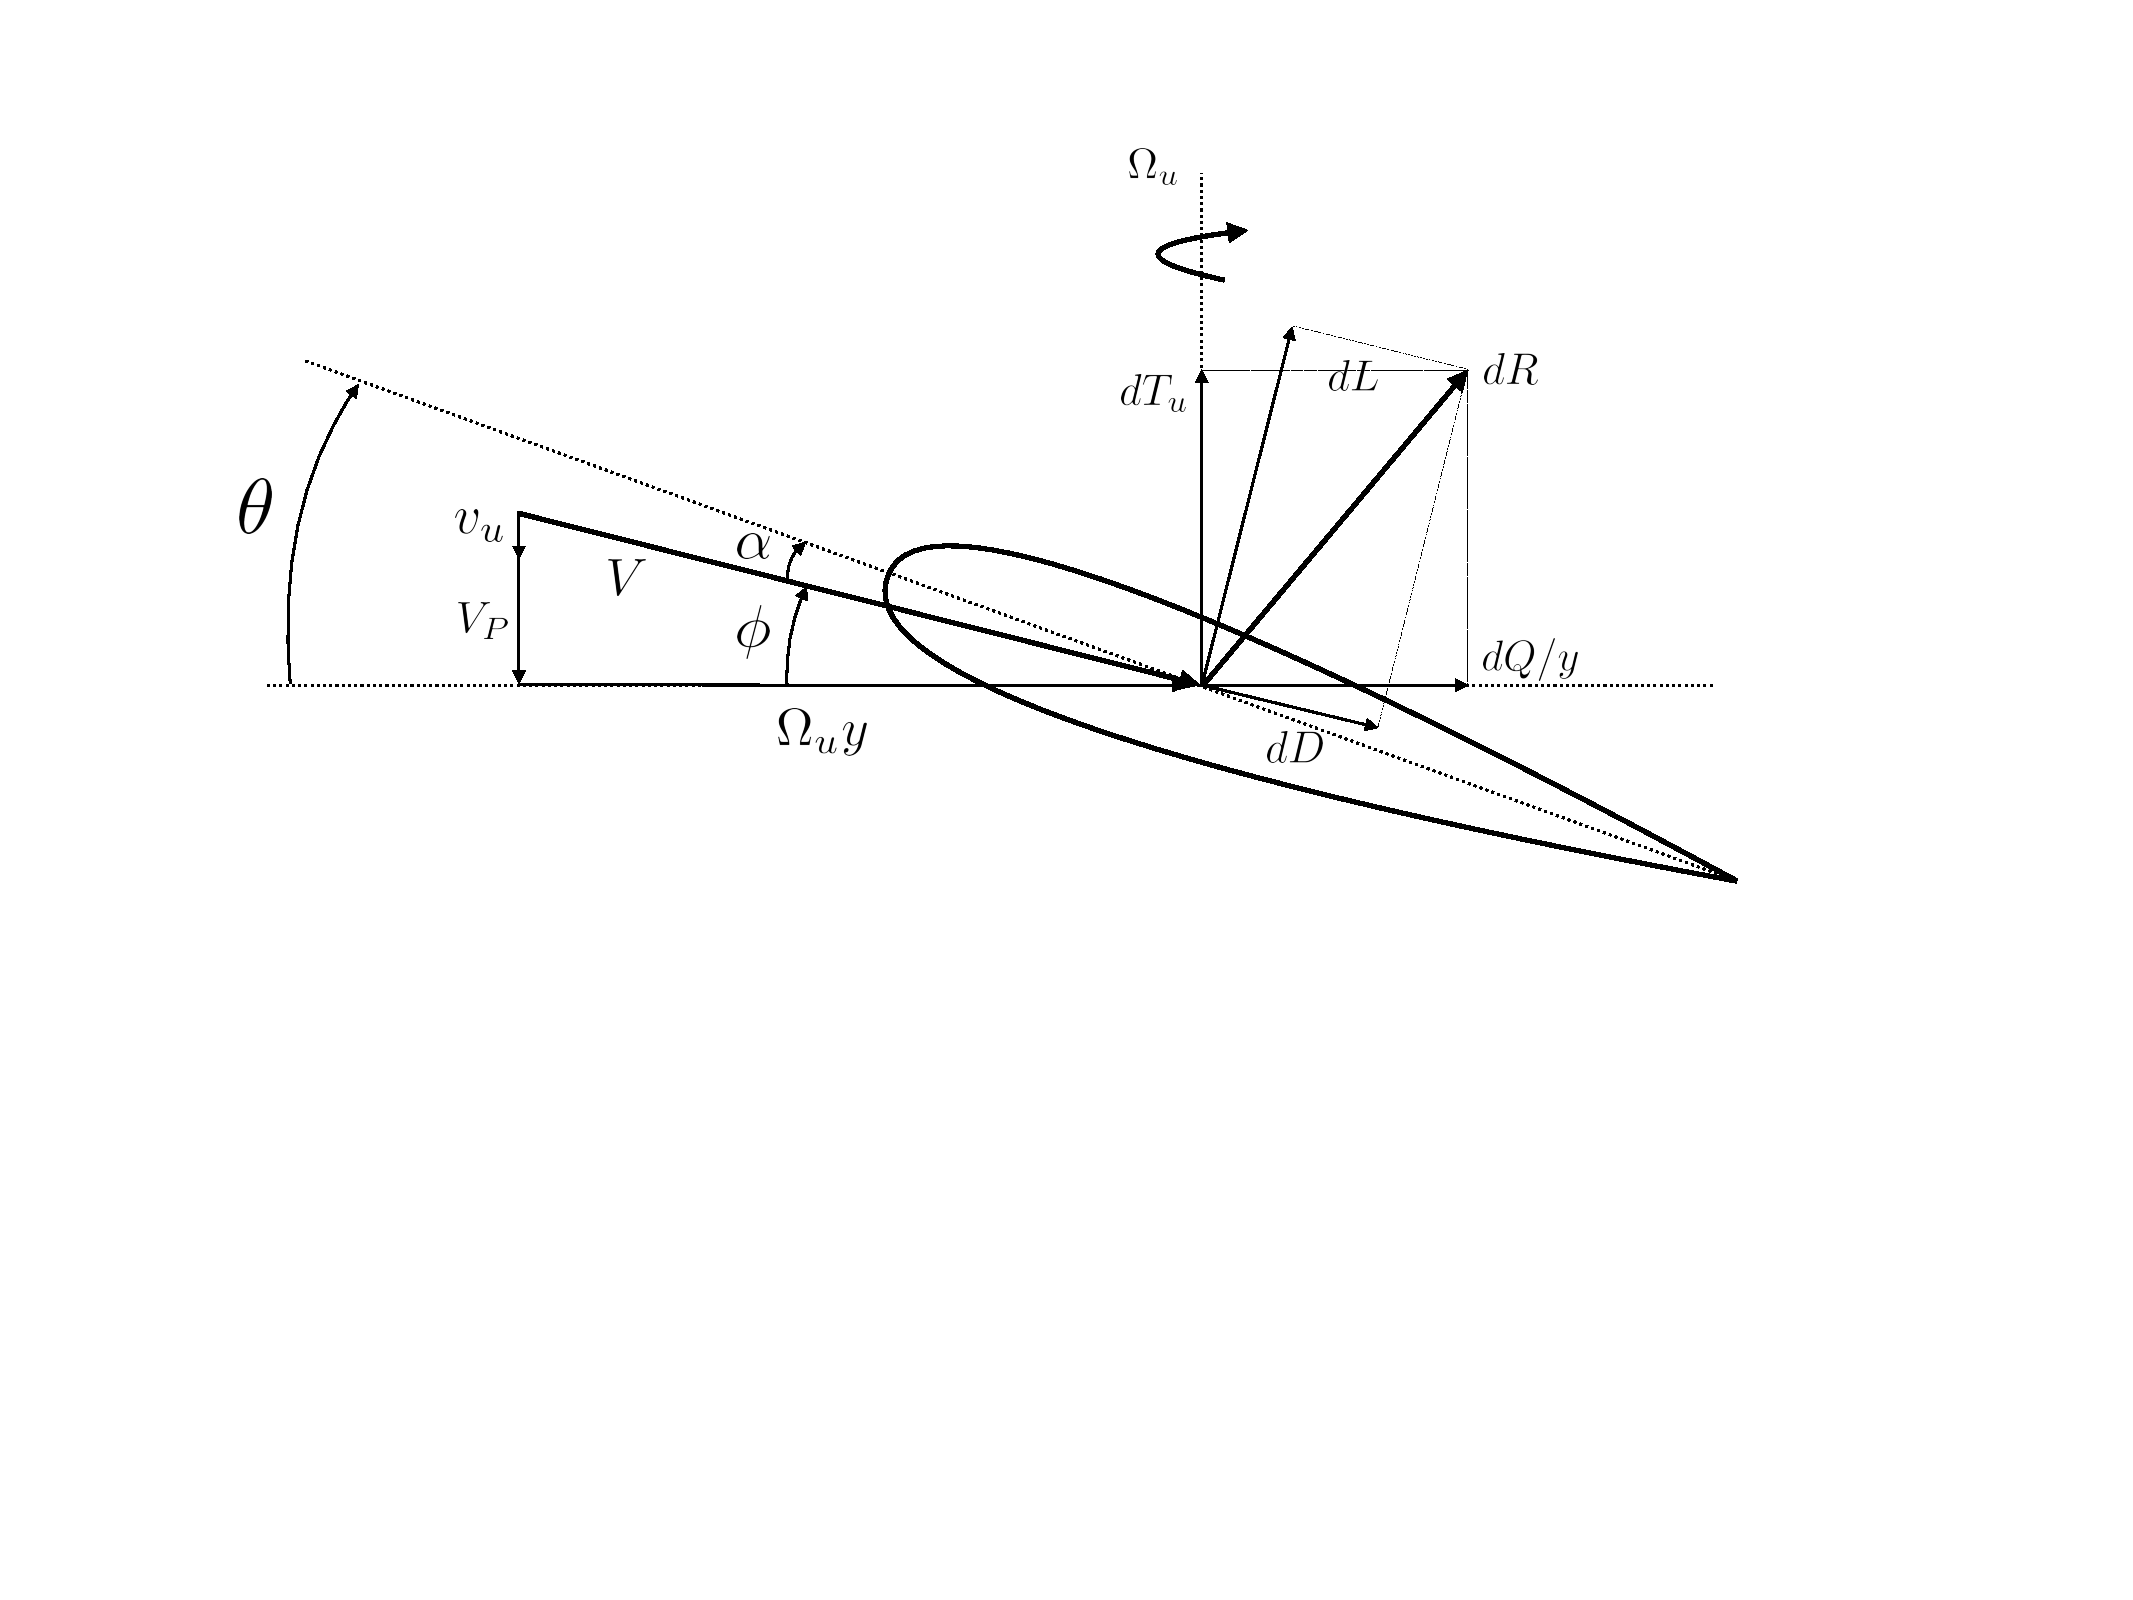
\includegraphics[width=\textwidth]{Figures/blade_axial.pdf}
    \caption{Cross-section of a blade element on the upper rotor}
    \label{fig:blade2d}
\end{subfigure}
\begin{subfigure}[t]{0.5\textwidth}
    \centering
    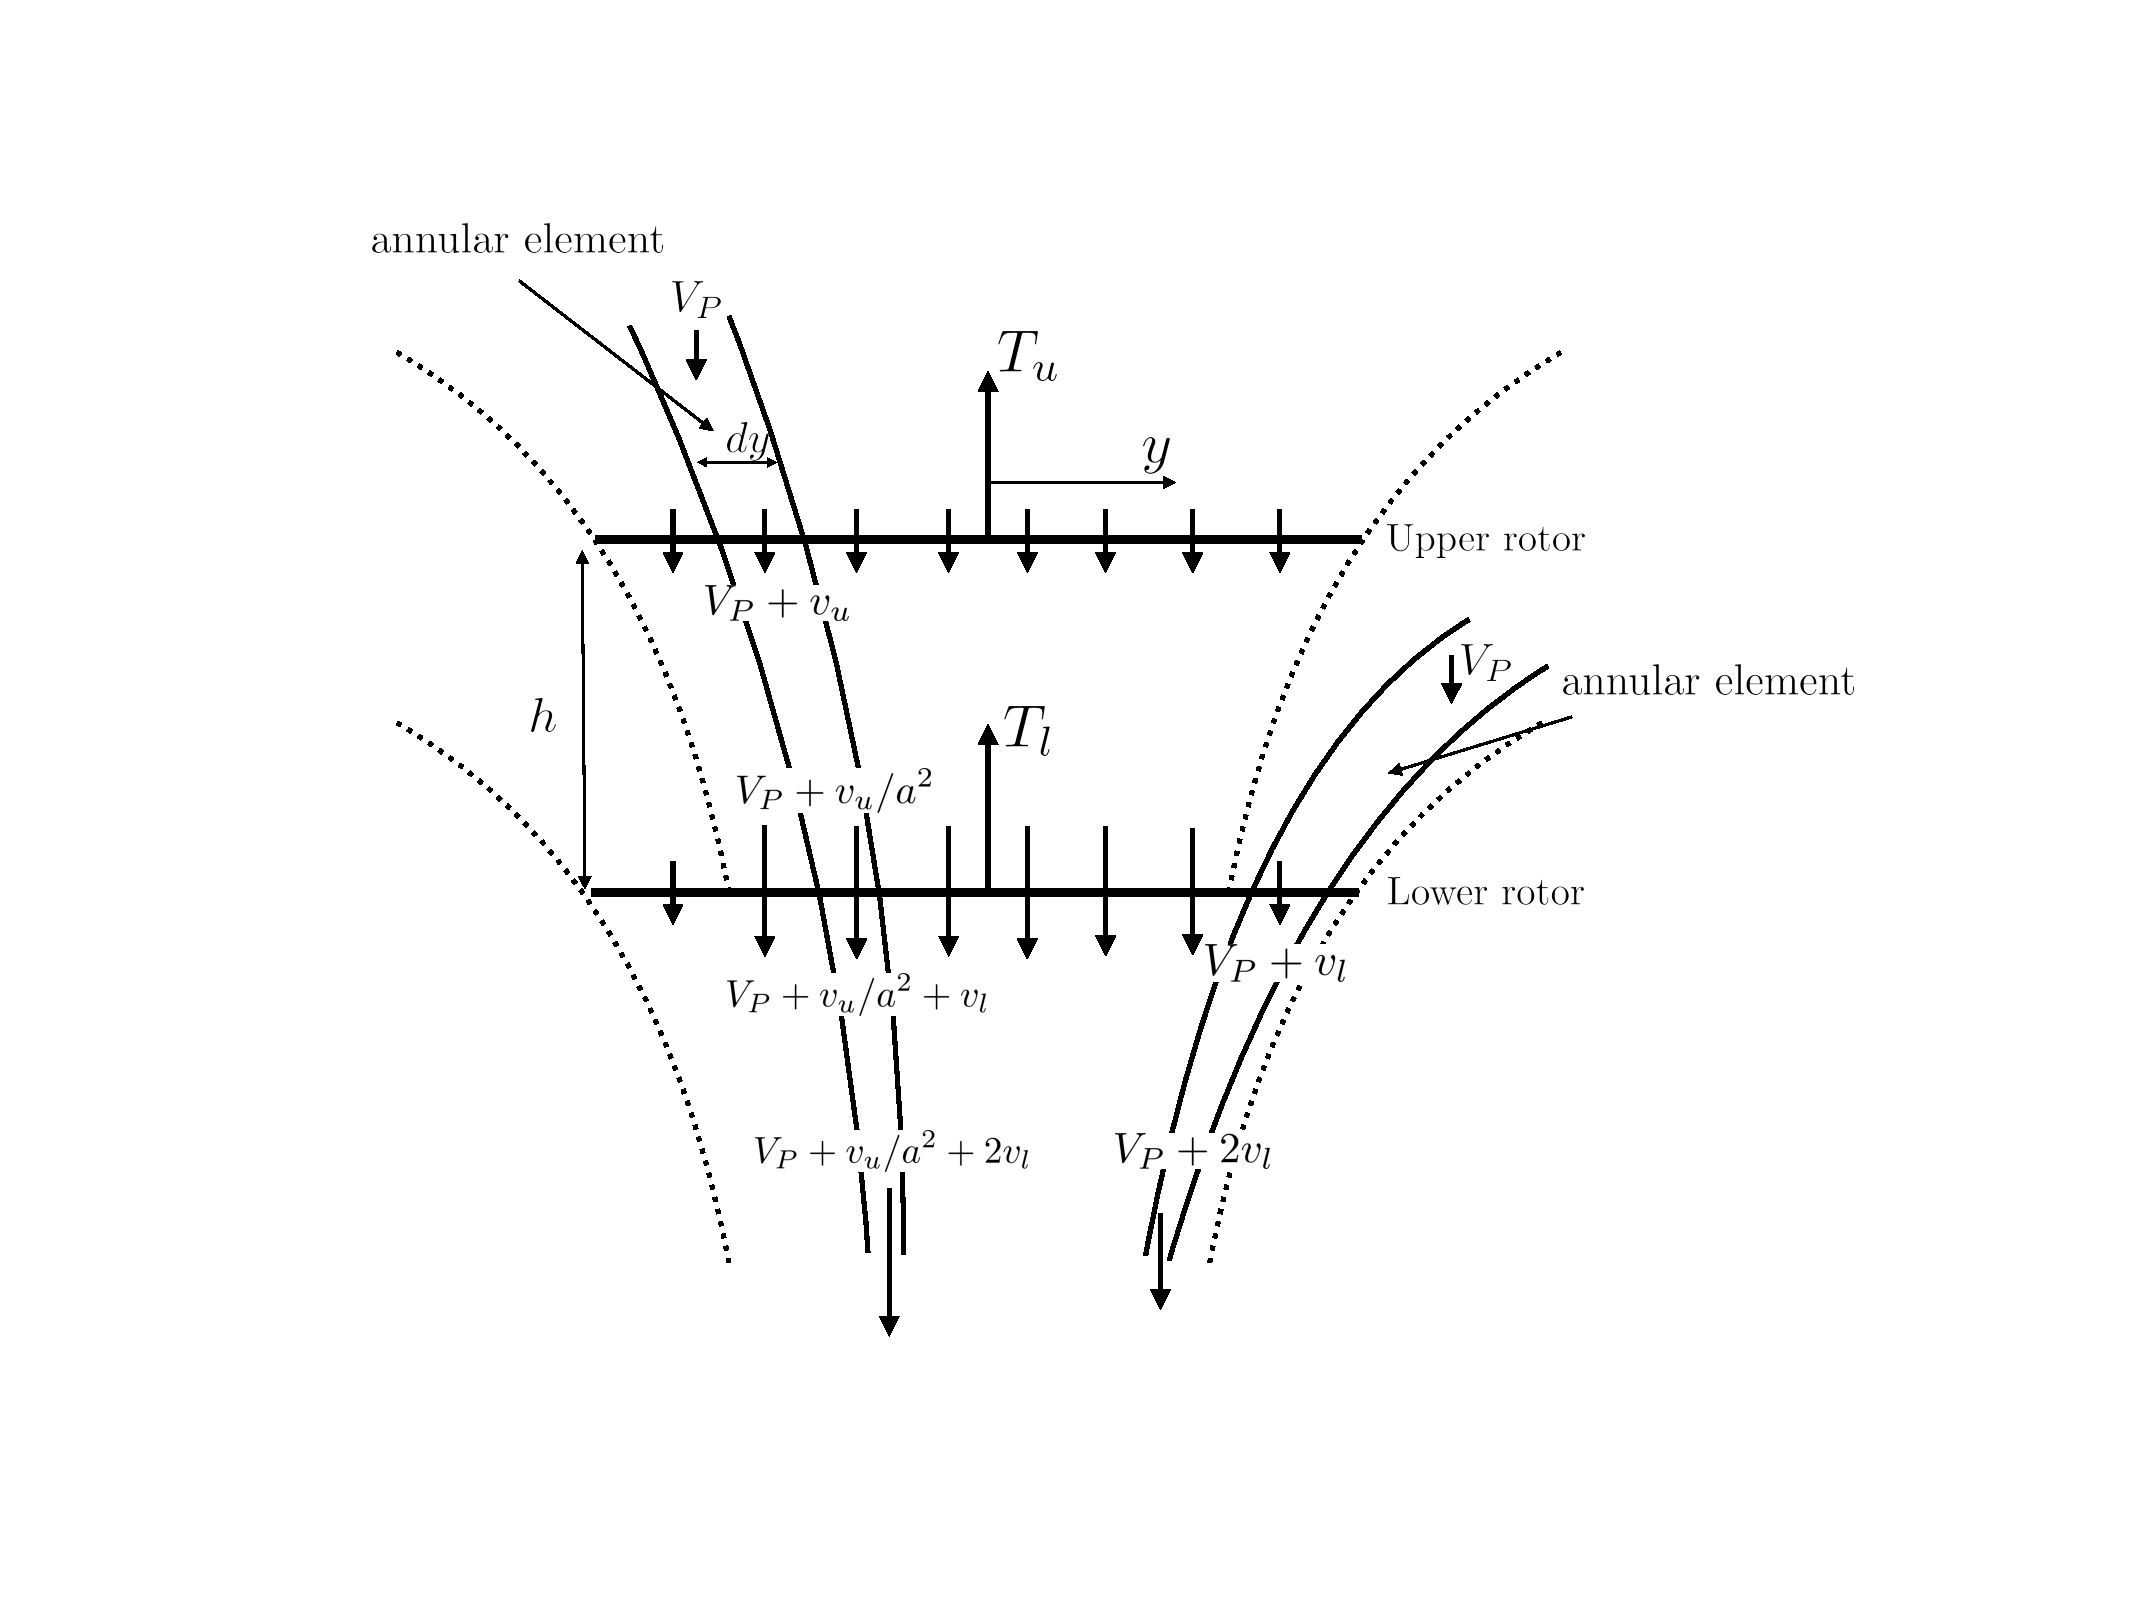
\includegraphics[width=\textwidth]{Figures/disk2D_BEM_axial.pdf}
    \caption{Flow model used for the BEMT analysis of a coaxial rotor system with the lower rotor operating in the slipstream of the upper rotor. }
    \label{fig:disks}
\end{subfigure}
    \captionsetup{justification=centering}
    \caption{Modelling approach for rotor blade elements in (a) and for the flow model in (b).}
    \label{fig:BEMT}
\end{figure}


For both a single and a coaxial rotor, the approach begins by considering the upper rotor. Momentum theory principles relate the thrust produced by an annulus to the product of the mass flow rate through it and the induced velocity there. The incremental thrust on the annulus is:

\begin{align}
 dT_u\, = 2d\dot{m}\, v_u \label{eq:dthrust} \\
  d\dot{m} = \rho(V_P+v_u)\,dA = 2\pi\rho(V_P+v_u)\,y\, dy,
\end{align}

where $d\dot{m}$ is the mass flow rate over the annulus, $V_P$ is the axial velocity of the rotor, $v_u$ is the induced velocity at a specific top rotor annulus, and $dA = 2\pi y\, dy$ is the area of a rotor annulus which is at a radial distance $y$ from the rotation axis of the rotor.

After non-dimensionalizing \autoref{eq:dthrust} by $\rho \pi R^2 (\Omega R)^2$, where $R$ is the rotor radius and $\Omega$ the rotational speed of the rotor, we obtain an expression for the thrust coefficient of the annulus:

\begin{align}
 dC_{T_u}\, = 4 F \lambda \lambda_u r dr \label{eq:dCthrust} 
\end{align}

where $r=y/R$, $\lambda= \lambda_P+\lambda_u = \frac{V_P+v_u}{\Omega R}$ and F is the Prandtl tip loss function:

\begin{equation}
 F\, = \frac{2}{\pi} \cos^{-1}(\exp(-f)). \label{eq:prandtl} 
\end{equation}

f is a function of the number of blades $N_b$, the radial position of the blade element r, and the inflow angle $\phi$ (equal to $\lambda(r)/r$ with a small angle assumption):

\begin{equation}
 f\, = \frac{N_b}{2} \Big(\frac{1-r}{r \phi} \Big) \label{eq:f}
\end{equation}

Using the circulation theory of lift, with small angle assumptions, \autoref{eq:dCthrust} can be equated to:

\begin{align*}
    dC_{T_u}\, = \frac{1}{2} \sigma_u r^2 dr = \frac{1}{2} \sigma_u C_{l_\alpha}(\theta_u-\phi-\alpha_0) r^2 dr \\
    = \frac{\sigma_u C_{l_\alpha}}{2}(\theta_u r^2 -\lambda r) dr  \numberthis
    \label{eq:dCthrust_circ} 
\end{align*}

where $\theta_u$ is the blade pitch distribution on the upper rotor, as shown in \autoref{fig:blade2d}. $\alpha_0$ and $C_{l_\alpha}$ are the zero-lift angle of attack and the lift curve slope of the airfoil at that blade section, respectively. $\sigma_u$ is the solidity of the upper rotor. 

Combining the expressions from \autoref{eq:dCthrust} and \autoref{eq:dCthrust_circ} allows to solve for the non-dimensionalized inflow ratio at the rotor annulus:

\begin{equation}
    \lambda(r,\lambda_P) = \sqrt{\Big(\frac{\sigma_u C_{l_\alpha}}{16 F}-\frac{\lambda_P}{2}\Big)^2+\frac{\sigma_u C_{l_\alpha}}{8F}\theta_u r} - \Big(\frac{\sigma_u C_{l_\alpha}}{16 F}-\frac{\lambda_P}{2} \Big).
\end{equation}

Since $\lambda$ is a function of $F$ and viceversa, a fixed-point iteration (which typically takes 5-10 iterations to converge) is performed to solve for $\lambda$ and consequently for $dC_{T_u}$, based on an initial guess of F=1. The incremental power coefficient can be found as the sum of induced and profile sources:

\begin{equation}
    dC_{P_u} = \lambda_u dC_{T_u} + \frac{1}{2} \sigma_u C_d r^3 dr
\end{equation}

where $C_d$ is the sectional profile drag coefficient. In this first analysis, $C_d = C_{d_0} + D_1 \alpha + D_2 \alpha^2$ and $D_1 = D_2 = 0$, which is a reasonable approximation for moderate values of blade loading coefficient \cite{BEMT}.

The approach for a coaxial rotor for the top rotor is exactly the same as the approach presented above (which is valid for a single isolated rotor). This assumes that the lower rotor does not affect the convergence of induced velocities on the top rotor. For the lower rotor, the approach for calculating incremental thrust and power coefficients is very similar to the method for the lower rotor. The only difference is that a distinction is made between the radial sections that ingest the contracted downwash of the upper rotor and the ones that do not.

\paragraph{Verification of the tool}


To verify the tool, the Harrington 1 coaxial rotor parameters were input into the tool, and the results for radial distribution of inflow, power/torque and thrust coefficients were compared at torque balance and a uniform pitch distribution (no twist) of 8 degrees. The comparison is shown in  \autoref{fig:verification_thrust} for the thrust coefficients. 

There is almost an identical correspondence for the inflow distribution and thrust coefficient plots. However, the power coefficients in the implemented BEMT seem to be overestimated (even though they have the correct order of magnitude). This means that for a fixed value of thrust required from a rotor, the torque required will be overestimated, which will increase the noise signature.

After quantifying the effect of this inaccuracy on the outputs of the tool which are design criteria (such as noise), it will be decided how much effort should go into improving the accuracy of the current BEMT.




%For a single rotor, the lower rotor in the diagram of \autoref{fig:disks} can be removed and the rest remains unchanged.


\paragraph{Future extensions}

As mentioned previously, the tool as is is is not being used to its full potential. In later stages of the design it will be used to optimize the propulsion system of the winning concept.

Currently, it is being used only in hover, but for proper optimization it will have to model the rotor in forward flight as well. An extension to the model presented in \cite{BEMT} will have to be made, which is currently only valid in hover and axial flight.

%Extend to forward flight.
 %Sensitivity to omega and Q
 
\begin{comment}

\begin{figure}
\captionsetup[subfigure]{justification=centering}
\begin{subfigure}[t]{0.5\textwidth}
    \centering
    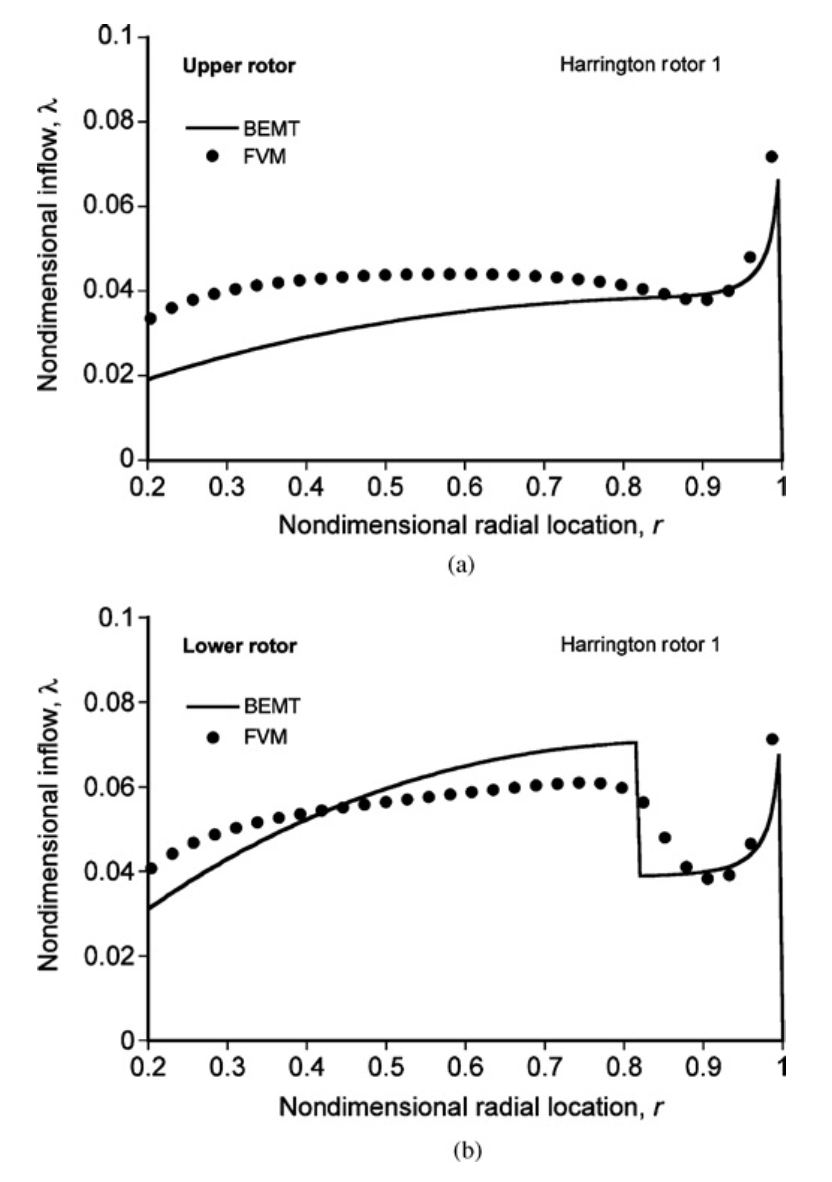
\includegraphics[width=\textwidth]{Figures/Leishman_inflow.png}
    \caption{Spanwise inflow distribution prediction by the BEMT in \cite{BEMT} and the Maryland Free Vortex Model in hover (torque balance)}
    %\label{fig:blade2d}
\end{subfigure}
\begin{subfigure}[t]{0.5\textwidth}
    \centering
    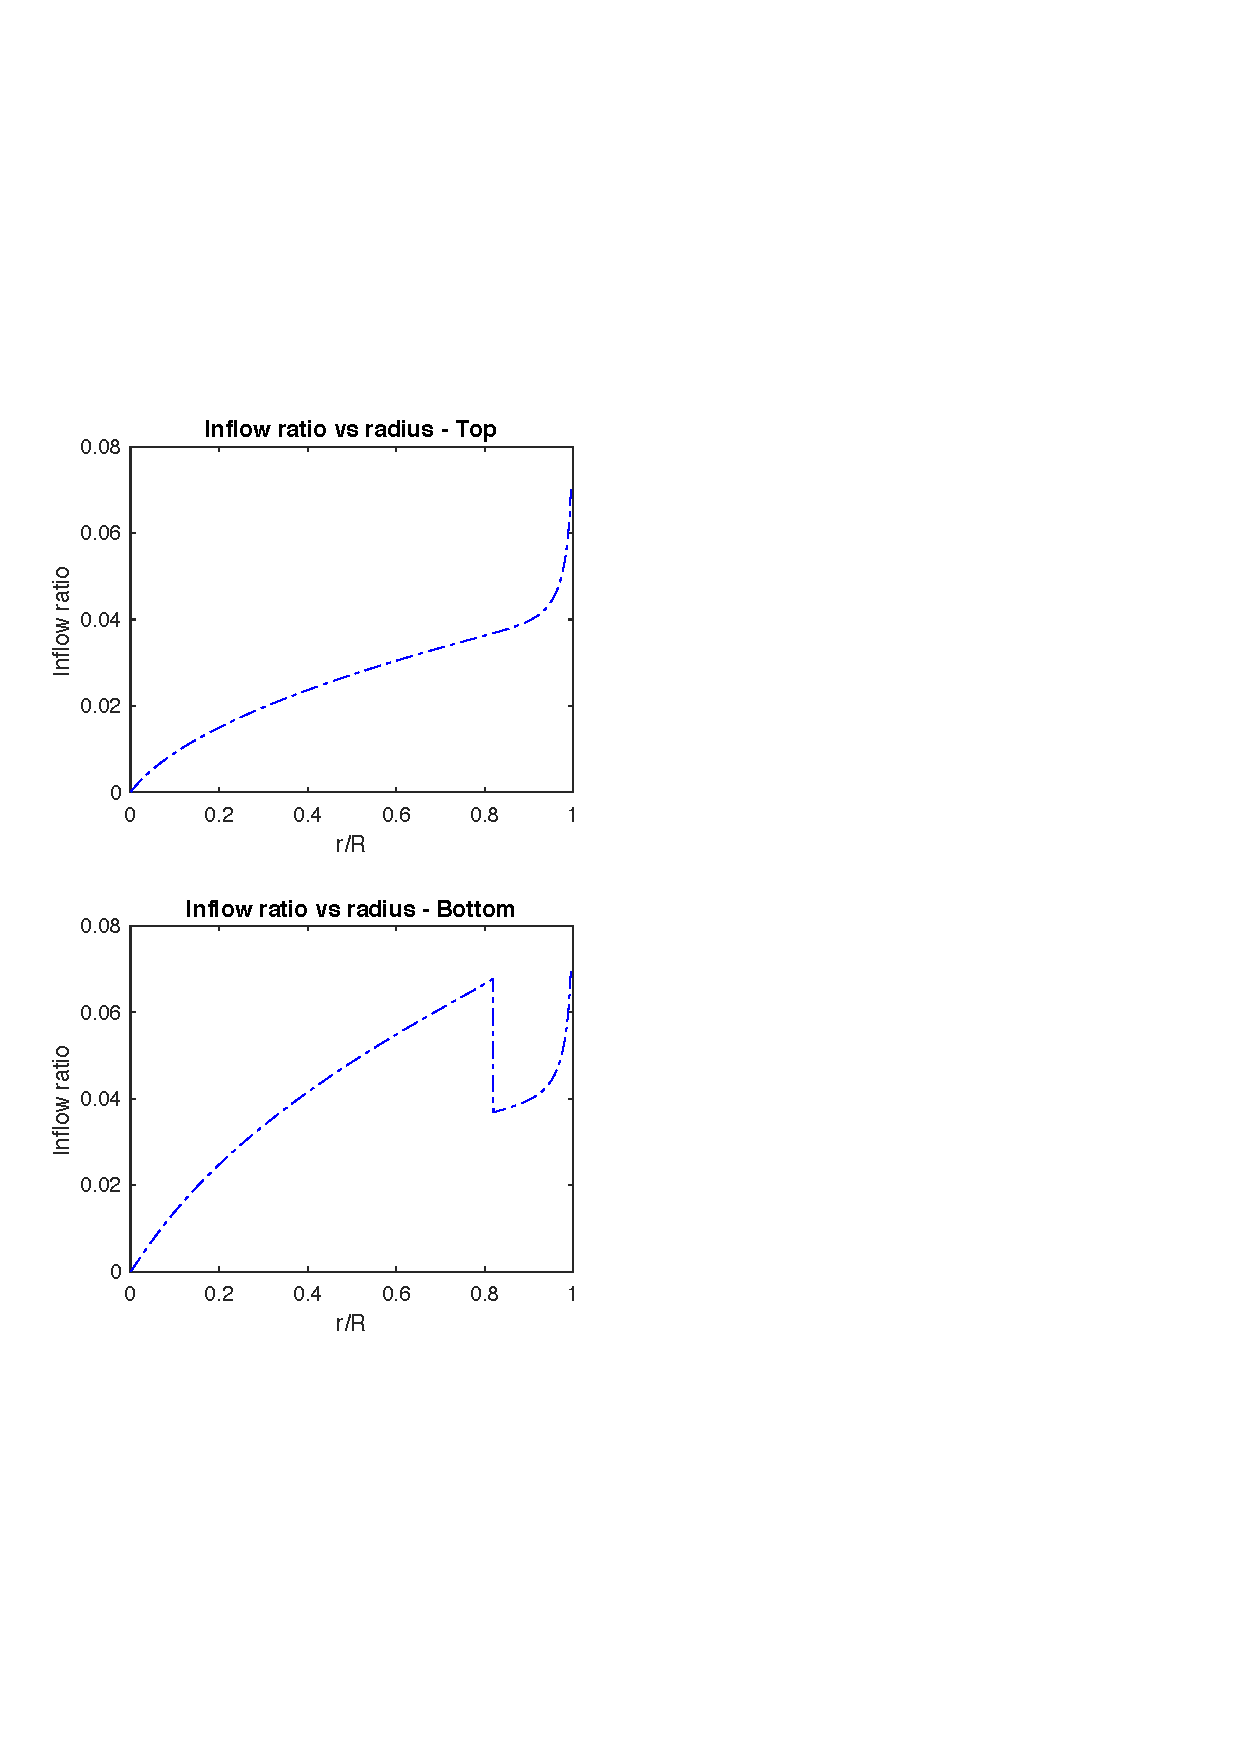
\includegraphics[width=\textwidth]{Figures/verification_inflow.pdf}
    \caption{Spanwise power coefficient prediction by implemented BEMT tool in hover (torque balance)}
    %\label{fig:disks}
\end{subfigure}
    \captionsetup{justification=centering}
    \caption{Verification plots for upper and lower rotor inflow distribution prediction of the Harrington 1 rotor.}
    \label{fig:verification_inflow}
\end{figure}

\end{comment}

\begin{figure}
\captionsetup[subfigure]{justification=centering}
\begin{subfigure}[t]{0.5\textwidth}
    \centering
    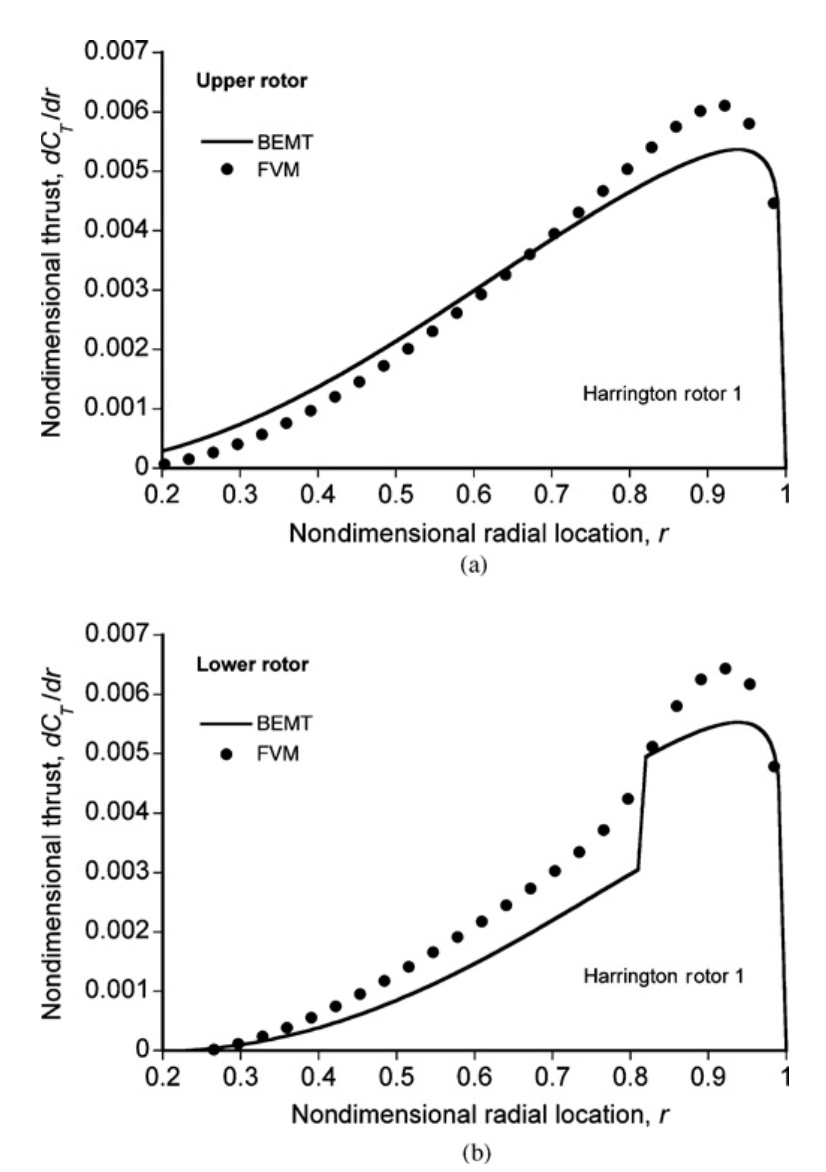
\includegraphics[width=\textwidth]{Figures/Leishman_CT.png}
    \caption{Spanwise thrust coefficient prediction by the BEMT in \cite{BEMT} and the Maryland Free Vortex Model in hover (torque balance)}
    %\label{}
\end{subfigure}
\begin{subfigure}[t]{0.5\textwidth}
    \centering
    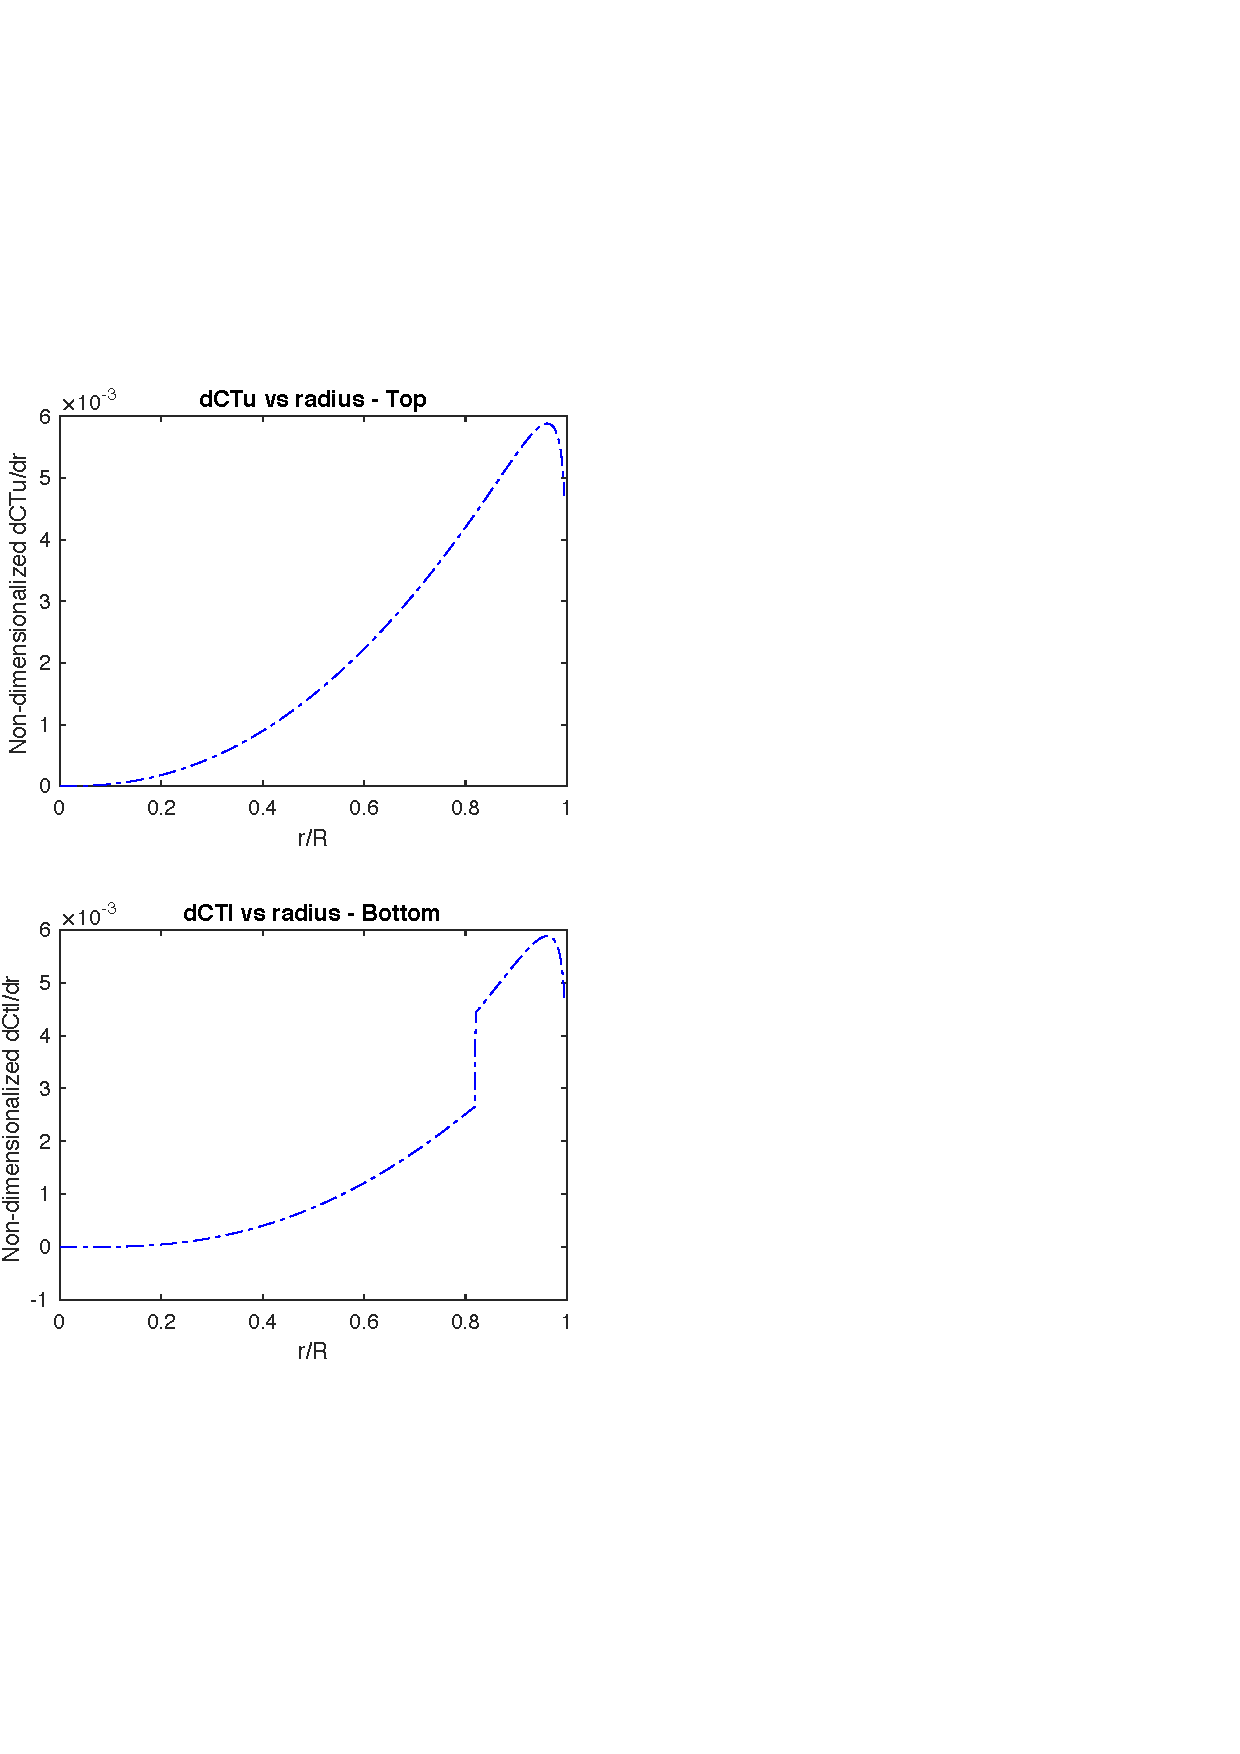
\includegraphics[width=\textwidth]{Figures/CT_plot.pdf}
    \caption{Spanwise power coefficient prediction by implemented BEMT tool in hover (torque balance)}
    %\label{fig:disks}
\end{subfigure}
    \captionsetup{justification=centering}
    \caption{Verification plots for upper and lower rotor thrust coefficient prediction of the Harrington 1 rotor.}
    \label{fig:verification_thrust}
\end{figure}

\begin{comment}


\begin{figure}
\captionsetup[subfigure]{justification=centering}
\begin{subfigure}[t]{0.5\textwidth}
    \centering
    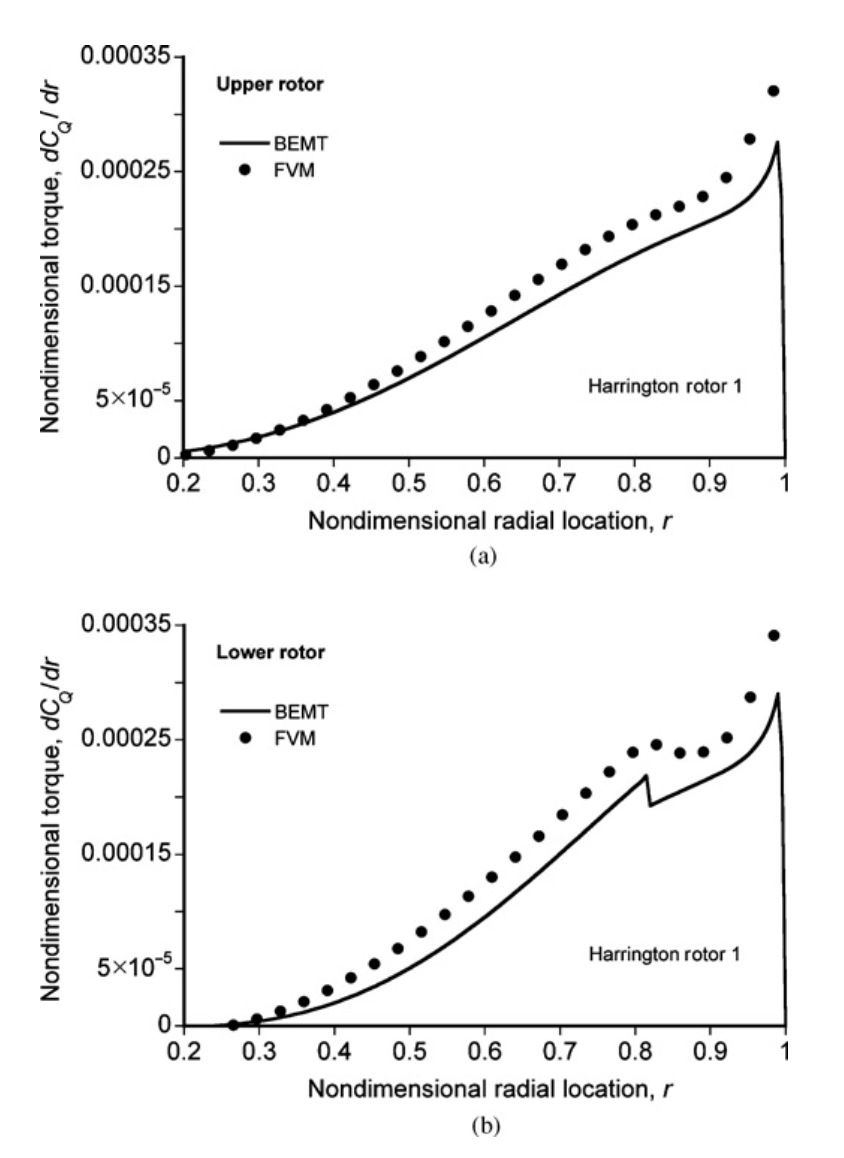
\includegraphics[width=\textwidth]{Figures/Leishman_CP.png}
    \caption{Spanwise power coefficient prediction by the BEMT in \cite{BEMT} and the Maryland Free Vortex Model in hover (torque balance)}
    %\label{fig:blade2d}
\end{subfigure}
\begin{subfigure}[t]{0.5\textwidth}
    \centering
    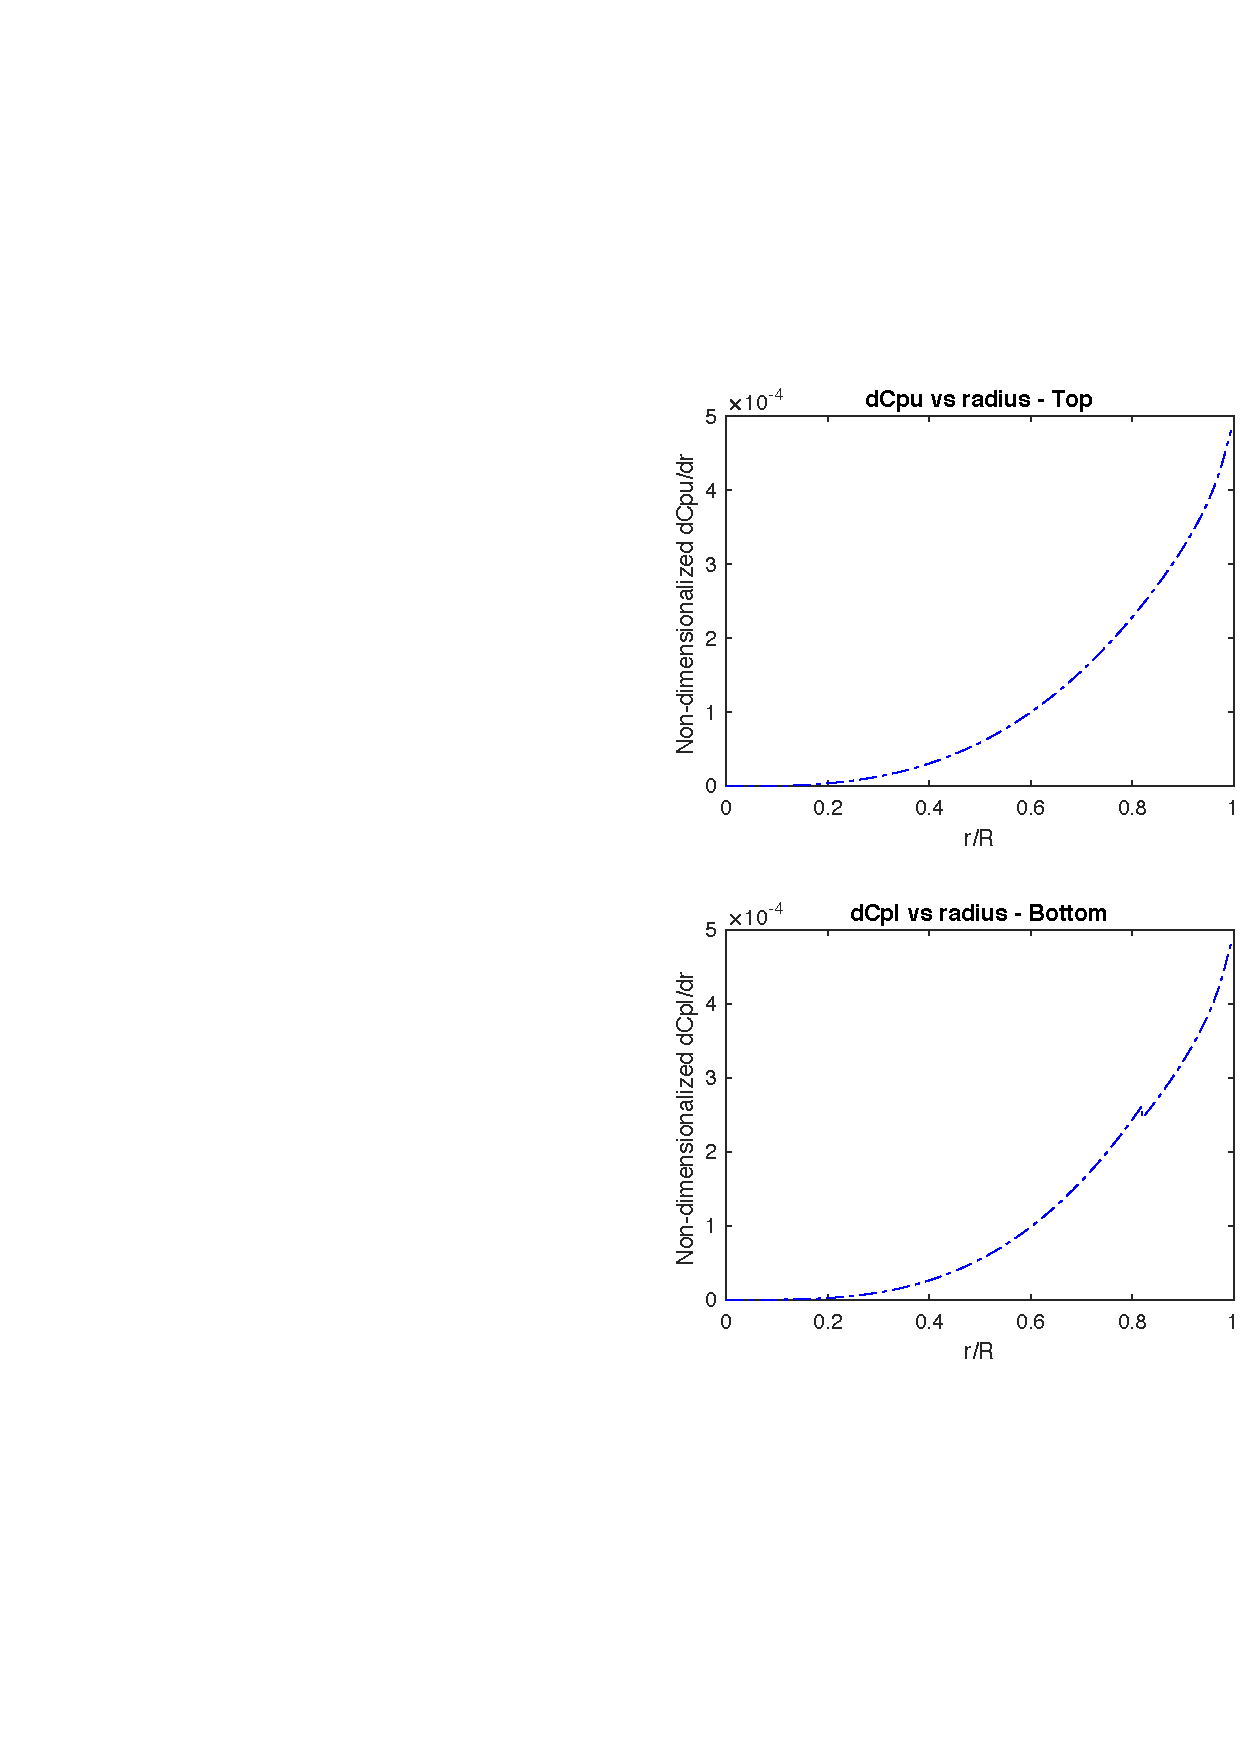
\includegraphics[width=\textwidth]{Figures/CP_plot.pdf}
    \caption{Spanwise power coefficient prediction by implemented BEMT tool in hover (torque balance)}
    %\label{fig:disks}
\end{subfigure}
    \captionsetup{justification=centering}
    \caption{Verification plots for upper and lower rotor power coefficient prediction of the Harrington 1 rotor.}
    \label{fig:verification_torque}
\end{figure}

\end{comment}

\subsection{Vehicle Noise}

The noise tool implemented for this stage of the project is based on \cite{Brown2018}, which presents a procedure for estimating harmonic and vortex noise for a rotorcraft in hover.


\paragraph{Harmonic Noise} is also referred to as rotational or tonal noise and can be divided into loading noise, which is a direct consequence of thrust generation, and thickness noise, caused by finite rotor blade thickness. What makes this type of noise characteristic is that it is emitted at discrete frequency harmonics of the fundamental frequency (which is $\Omega B$ for a single rotor and $\Omega_u B_u+ \Omega_l B_l$). Appendix C in \cite{Brown2018} derives the Gutin and Deming formulae in equivalent-radius form. They are presented here in final form for brevity:

\begin{align}
    p_{m_L} = \frac{mB\Omega}{2\sqrt{2}\pi a (\Delta S)} \Big(T \cos \theta - Q \frac{a}{\Omega R_e^2} \Big) J_{mB}\Big(\frac{m B \Omega}{a} R_e \sin \theta \Big) \\
    p_{m_T} = \frac{-\rho (m B \Omega)^2 B}{3 \sqrt{2} \pi (\Delta S)} c t R_e J_{mB} \Big(\frac{m B \Omega}{a} R_e \sin \theta \Big) \\
    SPL = 10 \log_10 \bigg[N \bigg(\frac{p_{m_L}^2+p_{m_T}^2}{p_{ref}^2} \bigg) \bigg]
\end{align}

$p_{m_L}$ and $p_{m_T}$ are the root mean square (RMS) sound pressures for loading and thickness noise, respectively. $m$ is the harmonic number (a positive integer), $N$ is the number of rotors, $B$ is the blade number per rotor, $\Omega$ is the rotor angular velocity (which is found in the BEMT tool in an iteration), $a$ is the speed of sound, and $\Delta S$ is the distance between the rotor and the observer. $T$ is the rotor thrust, $Q$ is the rotor torque (also coming from the BEMT), and $\theta$ is the elevation angle (in rad) plus $\frac{pi}{2}$ between the observer and the rotor hub. $\rho$ is the air density, $c$ is the blade chord and $t$ is the blade maximum thickness. $J_{mB}$ is a Bessel function of the first kind of order $mB$. An effective rotor radius of $R_e = 0.8 R$ is recommended in \cite{Brown2018} and is an assumption that approximates the integral that should be used for more accurate predictions. These improvements will be implemented in the next phase of the design phase if deemed necessary.


\paragraph{Vortex Noise}, also referred to as broadband noise is (as the name suggests) broadband in nature (continuous frequency spectrum). A model for vortex noise is derived in Appendix D A of reference \cite{Brown2018}, but is only presented in final form here:

\begin{align}
    SPL = 20 \log_10 \bigg[ K_2 \frac{V_T}{\rho (\Delta S)} \sqrt{\frac{NT}{s} \Big(\frac{T}{A} \Big)} \bigg] \\
    f_{peak} = \frac{(V_{0.7}\text{St})}{h}
\end{align}

where $T/A$ is the rotor disk loading; $K_2$ is a semi-empirical constant. Although vortex noise is broadband it has a peak frequency $f_{peak}$, which is a function of 0.7 times the tip speed, the projected blade thickness $h$ and the Strouhal number St. With the peak frequency known, the vortex-noise frequency spectrum can be obtained using the method in Appendix D B of \cite{Brown2018}.


\paragraph{A-Weighting Scheme}

Human ears have different responses at different frequencies. When it comes to social acceptance, it is more fitting to choose dBA as a metric for perceived sound pressure level, since it amplifies sounds being emitted close to 3kHz. Appendices B and D C in \cite{Brown2018} give a procedure on how to apply the weighting for tonal and vortex noise, respectively.

\paragraph{Atmospheric Attenuation}

On top of the procedure for noise prediction outlined in \cite{Brown2018}, a model for atmospheric attenuation based on frequency of emitted sound and atmospheric parameters was implemented \footnote{\url{ https://en.wikibooks.org/wiki/Engineering_Acoustics/Outdoor_Sound_Propagation} accessed on 20/05/2019.}.



\paragraph{Limitations}

\begin{itemize}
    \item Blade slap neglected, under the assumption that the tip Mach number stays below the transonic range (flags show up in the code if a particular concept does).
    \item The theory is not compatible with coaxial rotors. It most likely underestimates the noise for coaxial rotors. 
    \item The tool does not simulate destructive interference between sound sources. This is a fair assumption only if the sound emitted from these sources is of different frequencies.
    \item The effect of ducts and ground reflectance is not modelled.
\end{itemize}
 
\paragraph{Verification}

A thorough verification as done for the BEMT tool could not be performed due to time constraints. However, the article that the tool is based on does provide the parameters of the vehicles in the study and their noise signature, which will be used in the future to verify the accuracy of the tool. That being said, the outputs of the tool have realistic magnitudes and seem to behave as expected. For instance, the sensitivities of MTOW and noise always show that the noise increases when the MTOW increases, which is intuitively logical and can be extracted from the equations presented above. For vehicles with rotors that have low fundamental frequencies the noise footprint in dBA is lower than in dB, which also makes sense if one looks at the A-weighting curve which peaks at around 3 Hz. Many more of these sanity checks have been performed during tool integration and show up in the sensitivity studies. However, due to report space constraints, the plots for these sensitivities are not shown.


Sensitivity on Re (integration assumption)











\subsection{Downwash}
The downwash that is created by the propulsion system will be a factor in the social acceptance of a UAM system. It will be most critical in the take off phase of the flight. A large downwash will disturb day to day business of an urban environment to a greater extent than a system with a small downwash. Also, it would increase the amount of clearance needed around the landing site. 

The tool that gives an estimate of the downwash is for a large part dependent on the the thrust that is required, $T_{req}$. This is in turn a function of the mass of the vehicle, $m_{veh}$, and the acceleration, $a$ that is desired of the vehicle. The latter will be the result of a requirement on take-off velocity or time. According to Newton's second law 

\begin{equation}
\label{downwasheq}
    T_\text{req} = m_\text{veh} \cdot a + m_\text{veh} \cdot g 
\end{equation}

The area covered by the rotor is another input that is needed. The velocity of the air at the rotor can be computed with the fundamental principles of momentum and energy, from which \autoref{fancyconservationlaws} follows.

\begin{equation}
\label{fancyconservationlaws}
    T_\text{req} = \rho\cdot A_\text{rotor}\cdot(V + u_1)\cdot u_3 
\end{equation}

% A sketch of the situation is shown below

% \begin{figure}[H]
%     \centering
%     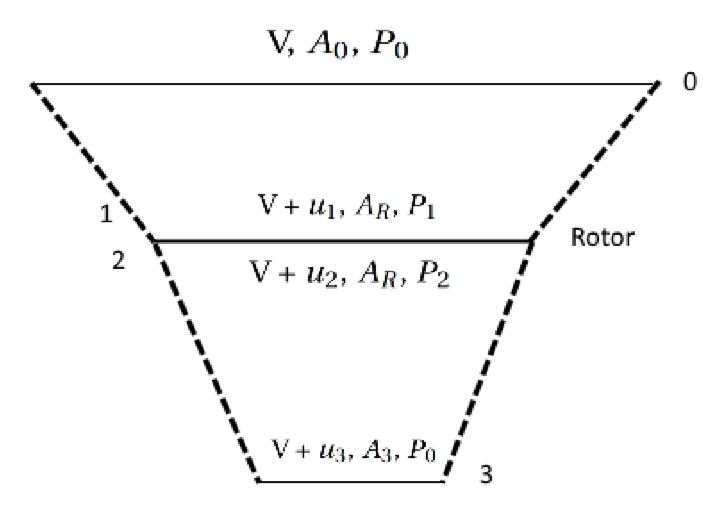
\includegraphics[width=0.5\linewidth]{Figures/downwashsketch.JPG}
%     \captionsetup{justification=centering}
%     \caption{Sketch of downwash computations}
%     \label{downwashsketch}
% \end{figure}

The expression in \autoref{u1u3} can be substituted into \autoref{fancyconservationlaws}. This equation follows from momentum theory. 

\begin{equation}
\label{u1u3}
    u_3 = 2\cdot u_1
\end{equation}

Then, $u_1$ is computed using by solving the quadratic equation. $u_3$ is easily found and one obtains the velocity of an air column at such as distance away that the pressure has returned to ambient levels. The area of that column can be computed with conservation of mass. The tool will be used to give an indication of the downwash for different concepts at this stage in the design and can be elaborated to compute the downwash of a vehicle concept in the detailed design phase. 

The downwash tool is fairly concise so the verification of this tool is trivial. Several unit tests can be performed. The first one is to double check whether the computed thrust makes sense, by looking at the computed values and the signs that are obtained. The next is to look if the found air velocities are correct. Here it's, just as in the thrust case, important to verify the sign. A positive flow velocity is defined as the case where the air moves through the rotor from up to down. The same holds for the mass flow. After these test are performed, the workings of the tool as a whole are verified by entering some extreme values, like zero and very large numbers, to check if the software doesn't report any errors.   


\begin{comment}
V, $A_{0}$, $P_{0}$ 

V + $u_1$, $A_{R}$, $P_{1}$

V + $u_2$, $A_{R}$, $P_{2}$

V + $u_3$, $A_{3}$, $P_{0}$
\end{comment}









\subsection{Route Selection and Passenger Throughput Requirement} \label{subsec:routeselection}

When working out, comparing and selecting different concepts, it is difficult to guarantee that the tools, metrics and criteria are not already biased to one of the system concepts. A simple example of this is the kind of and number of routes that the transportation system is designed to operate. A different set of routes requires a different systems to be optimally served, but maybe both are equally effective at solving congestion problems or being profitable. If the routes are fixed a priori, the emerging concept may be most suitable for these routes, but not most suitable at solving the mission need. However, the time scope of the project does not permit completely working out and designing all the concepts and finding their local optimum before selecting one. In the selection process itself, a trade-off was made between the fidelity of the system model and performance evaluation and the generality of that method. This is outlined in this section.


\paragraph{Revenue proxy}

An a priori proxy for revenue is set up based on trip time advantage with respect to cars on the same trip:

\begin{align} \label{eq:gainmetric}
    G(\text{trip}, t_\text{day}) = \left( T_{t_\text{car}}(\text{trip}, t_\text{day}) - T_{{t}_\text{UAM}}(\text{trip}) \right) \cdot \frac{\#\text{pax}(\text{trip},t_\text{day})}{D}
\end{align}

Here, $\#pax$ is the amount of people commuting the trip in question at the time of day in question and $D$ is the direct distance from origin to destination. The necessary data is known from the "Census Transportation Planning Products" (CTPP) \footnote{\url{https://ctpp.transportation.org/2012-2016-5-year-ctpp/} [accessed 08.05.19]}. This is the same data that was used to make a quantitative market analysis as described in \autoref{quantmarket}

\paragraph{Vehicle model}

The UAM trip time $T_{{t}_{UAM}}$ is estimated based on a simplistic; user specified model involving cruise speed, trip distance information and a constant estimate of boarding and first/last mile transport time. At a later stage when more about the vehicle and system concepts are known, iterations are possible on the trips that this UAM system should be designed using a more detailed model for the trip time.


\paragraph{Alternative (car) model}

From the more detailed market study of Los Angeles (\autoref{quantmarket}) a set of morning commutes is known showing the hourly flow of commuters between 113 districts. Because of the high combinatorics of this problem and available computational resources, the top $N = 2\ 800$ trips were sampled for each hour from 5am to 9am representing $75\%$ of the by-car commuters. These $14\ 000$ data points were queried to Google Maps' "Directions" API asking for the local time traffic-corrected and average traffic-corrected trip time on Monday the 13th of May, 2019. This puts numbers to the metrics $T_{t_\text{Car,avg}}$ and $T_{t_{\text{Car} }}(t_{day})$ and their ratio $C(t_{day}) = T_{t_{Car}}(t_{day}) / T_{t_\text{Car,avg}}$ as a congestion index for every of the $2\ 800$ trips.



\paragraph{Trip selection}

All known trips are sorted in descending order by metric \ref{eq:gainmetric} and stored in a table. The cumulative sum of the gain metric is defined as equation \ref{eq:gainsum}, with $0\leq n\leq N$ where $N$ is the total number of distinct trips available in the dataset. When a value for $n$ is selected, these top trips can be used as the design input for the system.

\begin{align} \label{eq:gainsum}
    S_n = \zeta \sum_{i=1}^{n}{G_i}
\end{align}

The constant factor $\zeta$ represents the percentage of the total people commuting these routes that are now transported by the UAM system. It is necessary, since it may depend on the mobility concept, whether all people on a small number of routes $n$ should be targeted, all a smaller percentage on a larger $n$.

$S_n$ can be set to a value $S_{\text{target}}$ which can be reached by setting appropriate values of the routes to serve $n$ and $\zeta$ with $S_{\text{target}} / \sum_{i=1}^{N}{G_i}\leq \zeta \leq 1$. Figure \ref{fig:zeta_n_demo} illustrates this concept. 

\begin{figure}
    \centering
    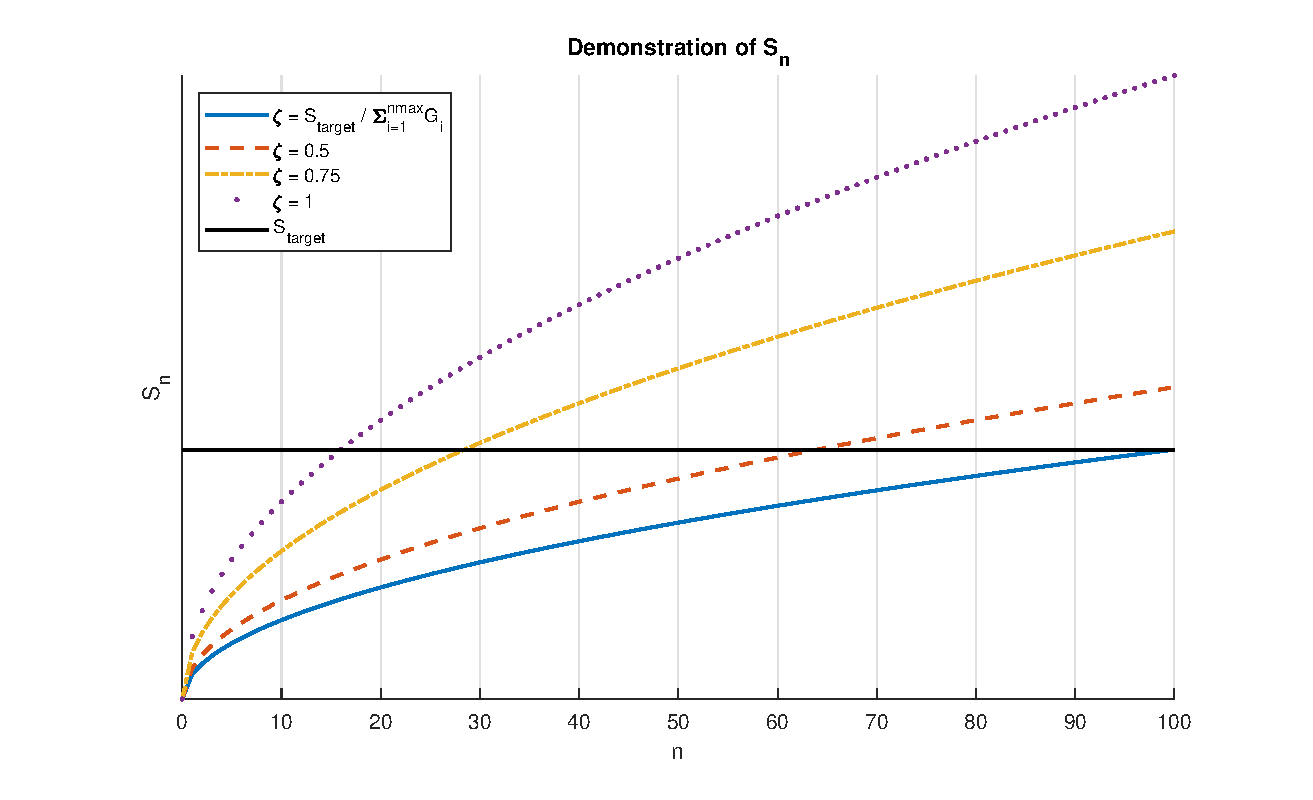
\includegraphics[width=0.8\textwidth]{Figures/S_nDemo.eps}
    \captionsetup{justification=centering}
    \caption{The target $S$ value can be reached by different combinations of $\zeta$ and $n$}
    \label{fig:zeta_n_demo}
\end{figure}


This procedure should relieve the bias and still make the outputs comparable between the different mobility system concepts: every system must provide the same "system gain" $S_n$, but the kind of routes and number of routes can be selected more freely to suit each concept while keeping the programming effort reasonably low and using the same tool for all concepts.

Now, that the $n$ "design trips" are known, the systems' performance can be evaluated on these trips using the other tools and the numbers for the list of trade criteria can be compiled. Iterations on the concepts' parameters can be performed, updating this list and also the trips for the UAM system.


\paragraph{Flux and Passenger Throughput}

 Furthermore, a metric called flux can be computed for all PUMA districts, based on the $n$ trips. This is the maximum of commuters flowing into a district and the outflow of commuters, as seen in equation \ref{eq:PUMAflux}:

\begin{align} \label{eq:PUMAflux}
    \begin{split}
    \Phi(\text{PUMA}_{in}, t_{day}) &= \sum_{i=1}^n{ \left( \text{pax}(\text{trip}_i, \text{into   PUMA}, t_{day})\right)}\\
    \Phi(\text{PUMA}_{out}, t_{day}) &= \sum_{i=1}^n{ \left( \text{pax}(\text{trip}_i, \text{out of PUMA}, t_{day})\right)}\\
    \Phi(\text{PUMA}, t_{day}) &= \text{max} 
    \left(
        \Phi(\text{PUMA}_{in}, t_{day}),
        \Phi(\text{PUMA}_{out}, t_{day})
    \right)
    \end{split}
\end{align}

This puts a preliminary throughput requirement on the throughput of a set of PUMAs which can be used to the subsequently compute an estimate of size and cost of the landing infrastructure necessary for this requirement with a certain vehicle capacity and turnaround or charging times. Also, a PUMA flux efficiency factor ($PFEF$) can be defined as the ratio of the minimum and maximum of the two scalars in equation \ref{eq:PFEF}; negative when more outflow, positive when more inflow ($-1 < PFEF < 1$). This will translate into the amount of zombie flight (flights without passengers) later and used in the infrastructure sizing.

\begin{align} \label{eq:PFEF}
    \begin{split}
        PFEF(\text{PUMA}, t_{day}) = &\frac{\text{min} 
        \left(
            \Phi(\text{PUMA}_{in}, t_{day}),
            \Phi(\text{PUMA}_{out}, t_{day})
        \right)
        }{\text{max} 
        \left(
            \Phi(\text{PUMA}_{in}, t_{day}),
            \Phi(\text{PUMA}_{out}, t_{day})
        \right)
        } \\
        &\cdot sgn ( \Phi(\text{PUMA}_{in}, t_{day}) - \Phi(\text{PUMA}_{out}, t_{day}) )
    \end{split}
\end{align}



\paragraph{Verification}

Since only $40\ 000$ of Google Maps API Directions queries were available free of charge from Google and $14\ 000$ are needed, care must be taken to verify the queries before issuing them to mitigate the risk of using up the queries accidentally without obtaining useful results. This was done by requesting the same information for a few randomly chosen trips manually on \url{www.google.com/maps} and via the API from MATLAB. After this succeeded and the information was confirmed to be identical, the integration was checked by using the final input and output files, but limiting the trips to 5 at random. Following this, a dry run was performed by formulating all queries and writing the output files as before, but without actually invoking the API. 

After enough confidence was established, the program ran in around 2 hours. However, when evaluating the average time loss due to traffic, the percentage (33\% of average trip time added) did not match the TomTom traffic index \footnote{\url{https://www.tomtom.com/en_gb/trafficindex/city/los-angeles}} which reports 62\% for the morning peak in 2016 (with an upwards trend in the recent years), at the same time of day as predicted by this algorithm (8am to 9am). To investigate this, the traffic model that Google provides was configured from "best-estimate" to "pessimistic". The $14\ 000$ items query was run again, resulting in FINISH THIS SENTENCE

To verify the flux calculations, a shortened trip definitions file was created and the fluxes manually computed for the low amount of trips. This was compared and confirmed to match with the scripted calculations and also associativity with the GEOIDS (specificing the location within LA country) was confirmed to be kept. Although not shown here for bevity, these unit testing files are available from us on request.



\iffalse
\subsection{Trip Time Gain}

In this tool it is assumed that the likelihood of people using a new UAM system is mainly related to the trip time advantage. This, however, may not be true alone but is an easy metric to quantify without running surveys or complex social-economic simulations and in this context only serves as a way to estimate an initial guess of the kinds of trips that a UAM vehicle is "good at". The vehicle model is kept as basic a possible in this tool. At a later stage when more about the vehicle and system concepts are known, iterations are possible on the trips that this UAM system should be designed for or it may turn out that other factors make some of the trips found here unsuitable or shift the focus to different metrics than trip time advantage.

\paragraph{Design}

It was evaluated on which trips exactly a UAM system provides large trip time advantage, to determine the routes and throughput necessary as a function of vehicle performance. This helps determining the vehicle characteristics necessary for a competitive system that increases the chance of solving congestion problems and puts requirements on the local infrastructure necessary.

A simple parametric vehicle model is able to determine the net trip time $T_{{net}_{UAM}}$ for a given distance (MORE ON THIS WHERE?). Adding a constant estimate of the constant trip time components $k$ (first mile/last mile/boarding) yields a very crude estimate of the total trip time $T_{{t}_{UAM}}$ that can be compared to other modes of transport.

From the more detailed market study of Los Angeles (\autoref{quantmarket}) a set of morning commutes is known showing the hourly flow of commuters between $113$ (IS THIS 113 OR 112?!) districts. Because of the high combinatorics of this problem and available computational resources, the top $2\ 800$ trips were sampled for each hour from 5am to 9am representing $75\%$ of the by-car commuters. These $14\ 000$ data points were queried to Google Maps' (MAKE SOME BRAND SYMBOL HERE) "Directions" API asking for the local time traffic-corrected and average traffic-corrected trip time on Mon 13, 2019. This puts numbers to the metrics $T_{t_{\text{Car},\text{avg} }}$ and $T_{t_{\text{Car} }}(t_{day})$ and their ratio $C(t_{day}) = T_{t_{Car}}(t_{day}) / T_{t_{\text{Car},\text{avg}} }$ as a congestion index for every of the $2800$ trips.

The same trips were computed for the simplistic vehicle model and the metric in equation \ref{eq:gainmetric} was applied to score the trips.

Ranking the top $n$ trips by this metric given an idea of the routes that a UAM would be most acceptable by people that want to save time on their commutes; the people we primarily target to diminish congestion. Furthermore, a metric called flux was computed for all PUMA districts which is maximum of commuters flowing into a district on one of these trips and the outflow of commuters.

\begin{align} \label{eq:PUMAflux}
    \begin{split}
    \Phi(\text{PUMA}_{in}, t_{day}) &= \sum_{i=1}^n{ \left( \text{pax}(\text{trip}_i, \text{into   PUMA}, t_{day})\right)}\\
    \Phi(\text{PUMA}_{out}, t_{day}) &= \sum_{i=1}^n{ \left( \text{pax}(\text{trip}_i, \text{out of PUMA}, t_{day})\right)}\\
    \Phi(\text{PUMA}, t_{day}) &= \text{max} 
    \left(
        \Phi(\text{PUMA}_{in}, t_{day}),
        \Phi(\text{PUMA}_{out}, t_{day})
    \right)
    \end{split}
\end{align}

This puts a preliminary throughput requirement on the throughput of a set of PUMAs which can be used to the subsequently compute an estimate of size and cost of the landing infrastructure necessary for this requirement with a certain vehicle capacity and turnaround or charging times. Also, a PUMA flux efficiency factor ($PFEF$) can be defined as the ratio of the minimum and maximum of the two scalars in equation \ref{eq:PFEF}; negative when more outflow, positive when more inflow ($-1 < PFEF < 1$). This will translate into the amount of "zombie" flight (flights without passengers) later and used in the infrastructure sizing.

\begin{align} \label{eq:PFEF}
    \begin{split}
        PFEF(\text{PUMA}, t_{day}) = &\frac{\text{min} 
        \left(
            \Phi(\text{PUMA}_{in}, t_{day}),
            \Phi(\text{PUMA}_{out}, t_{day})
        \right)
        }{\text{max} 
        \left(
            \Phi(\text{PUMA}_{in}, t_{day}),
            \Phi(\text{PUMA}_{out}, t_{day})
        \right)
        } \\
        &\cdot sgn ( \Phi(\text{PUMA}_{in}, t_{day}) - \Phi(\text{PUMA}_{out}, t_{day}) )
    \end{split}
\end{align}

\paragraph{Iterations}

This tool should primarily serve comparisons between system concepts (mainly number of passengers), but can later be used to compute more accurate estimates of time gain and throughput requirements, once an updated vehicle performance model is supplied.

Even later, when possible hub locations are known, the Google Maps query can be updated with more precise locations and trips.


\paragraph{Verification}

Since only $40\ 000$ of Google Maps API Directions queries were available free of charge from Google and $14\ 000$ are needed, care must be taken to verify the queries before issuing them to mitigate the risk of using up the queries accidentally without obtaining useful results. This was done by requesting the same information for a few randomly chosen trips manually on \url{www.google.com/maps} and via the API from MATLAB. After this succeeded and the information was confirmed to be identical, the integration was checked by using the final input and output files, but limiting the trips to 5 at random. Following this, a dry run was performed by formulating all queries and writing the output files as before, but without actually invoking the API. 

After enough confidence was established, the program ran in around 2 hours. However, when evaluating the average time loss due to traffic, the percentage (33\% of average trip time added) did not match the TomTom traffic index \footnote{\url{https://www.tomtom.com/en_gb/trafficindex/city/los-angeles}} which reports 62\% for the morning peak in 2016 (with an upwards trend in the recent years), at the same time of day as predicted by this algorithm (8am to 9am). To investigate this, the traffic model that Google provides was configured from "best-estimate" to "pessimistic". The $14\ 000$ items query was run again, resulting in FINISH THIS SENTENCE

To verify the flux calculations, a shortened trip definitions file was created and the fluxes manually computed for the low amount of trips. This was compared and confirmed to match with the scripted calculations and also associativity with the GEOIDS (specificing the location within LA country) was confirmed to be kept. Although not shown here for bevity, these unit testing files are available from us on request.
\fi



\subsection{System Size Estimation and Daily Footprint}

In the previous section \ref{subsec:routeselection}, the routes best served by a specific vehicle concept were estimated and a throughput requirement was established for each of these trips. This section addresses how this requirement flows down into more specific requirements like fleetsize and number of required vertiports. The system is sized for a share of the throughput of the morning peak which occurs around 8-9am in Los Angeles and the daily energy footprints and system usage is calculated assuming that all targeted commuters travel between 5am and 10am (the period that we have trip and traffic data for) and return in the afternoon, so multiplying the figures for the morning commutes by 2.

Another input to this subtool is the $\zeta$ factor which indicates the fraction of passengers served that go on the selected routes. Note that this is not the overall market share, which is estimated at the end of this section.


\paragraph{Vehicle Trip Model and Zombie Flights}

For any system, whether it is on-demand or scheduled, it must be taken into consideration that not every trip is served with full passenger payload. For the sake of simplicity, it is assumed throughout that each trip that a vehicle undertakes it is either fully loaded with passenger payload ("revenue flight") or is empty ("zombie flight") with only crew remaining, if applicable.

It proved difficult to include models of different ATM systems in the tools. This could have either been done by assuming a predefined zombie flight ratio and estimating this for different ATM concepts; however, not reliable or supported way of doing so could be determined. Another, more direct way would be to run an agent based simulation and optimise the trips based on demand, routes and the current vehicle positions and trajectories. \footnote{\url{https://www.bauhaus-luftfahrt.net/fileadmin/user_upload/2018_AIAA_Aviation_Rothfeld_Agent-based_UAM.pdf}} This, however, is outside the scope of this concept selection phase and so it was chosen to look at a hub to hub system for fleet size and ground structure estimation, while realising that certain vehicles concepts may benefit from one choice over the other. Therefore, the next section \ref{subsec:GateThroughput} takes different system choices into account, providing insights that help with the trade-off.

For the subsequent calculations it is assumed that every vehicle only goes back and forth between 2 hubs. The number of trips per unit of time $\Psi$ on a certain route $i$ is governed by the maximum of the passengers $pax$ on that route $R$ or its the inverse route $\bar{R}$ times two, see \autoref{eq:RouteFlow}. The metric $veh_{pax}$ indicates how many passengers can be carried by one vehicle. There are $m$ unique routes pairs (a pair is a route and its inverse) to iterate over.

\begin{align} \label{eq:RouteFlow}
    \text{maxveh} &= \ceil{ \max( \frac{pax(R_i)}{veh_{pax}} \zeta, \frac{pax(R_i)}{veh_{pax}}\zeta ) }\\
    \text{minveh} &= \ceil{ \min( \frac{pax(R_i)}{veh_{pax}} \zeta, \frac{pax(R_i)}{veh_{pax}}\zeta ) }\\
    \Psi(R\cup\bar{R}, t_{\text{day}}) &= 2\cdot \text{maxveh}
\end{align}

Notice, that in the case that there are no passengers demanding the return route, the zombie ratio $z$ is $0.5$. A more precise definition is given in \autoref{eq:zombierat}:

\begin{align} \label{eq:zombierat}
\begin{split}
    z(R\cup\bar{R}, t_{\text{day}}) &= \frac{\text{total trips - revenue trips}}{\text{total trips}} = \frac{(\Psi(R\cup\bar{R}, t_{\text{day}}) - (\text{maxveh} + \text{minveh}))}{\Psi(R\cup\bar{R}, t_{\text{day}})}
\end{split}
\end{align}


\paragraph{Passenger Kilometres and Energy}

For each trip at each of the 5 discrete time slots the required vehicle energy, air-time and turnaround time is calculated. The trip energy $E$ depends on whether the flight carries passengers or is a zombie flight, with the latter being significantly lower (\autoref{eq:EnergyTrip}). Passenger kilometres $\text{pax}_{km}$ on a certain route during a discrete time slot are simply the sum of the revenue trips multiplied with the route length $D$ as shown in \autoref{eq:paxkm}.

\begin{align} \label{eq:EnergyTrip}
\begin{split}
    E(R\cup\bar{R}, t_{\text{day}}) &= \Psi(R\cup\bar{R}, t_{\text{day}}) \cdot \left(E_{\text{zombie}} \cdot z + E_{\text{revenue}} \cdot (1-z) \right)
\end{split}
\end{align}

\begin{align} \label{eq:paxkm}
\begin{split}
    \text{pax}_{km}(R\cup\bar{R}, t_{\text{day}}) &= \left( \text{maxveh} + \text{minveh} \right) \cdot veh_{pax} \cdot D(R\cup\bar{R})
\end{split}
\end{align}


\paragraph{Fleet Sizing}

Now that the total number of trips on every route is known per unit of time (hour), the fleet size can be approximated if it is known how long vehicle takes to complete one flight cycle (take-off to take-off), summing over all chosen route. This time is approximated as the sum of air time $AT$, depending largely on the cruise speed and the turnaround time $TT$, depending on a boarding/deboarding/taxi constant, trip energy and charge rate (recharging is assumed to be performed before every flight for simplicity). More details on these time can be found in SECTION REFERENCE SOMETHING HERE as equation \autoref{eq:fleetsize}.

Here, wind and vehicle maintenance during the daily service time is neglected. This overhead surely needs to be taken into account when sizing the fleet for the final system design, but this simplified metric should serve for concept selection as it adequately compares the differences in fleet sizes for different vehicle definitions.

\begin{align} \label{eq:fleetsize}
    \text{fleet size} = \sum_{i=1}^m { \ceil{ \left( (AT + TT)_{i, \text{zombie}} \cdot z + (AT + TT)_{i, \text{revenue}} \cdot (1-z) \right) \cdot \Psi((R\cup\bar{R})_i, t_{\text{peak}}) } }
\end{align}


\paragraph{Hubs Sizing}

Knowing the vehicle flow per hour on every unique route enables sizing of the hubs as well. For simplicity, on "lumped" hub is placed at the centre of each served PUMA. The hub is variable in size and may contain a number of vertiports which are comprised of one landing/take-off pad and a number of gates where vehicles ground operation takes place ((de-)boarding, recharging, ...). For each hub, a weighted average turnaround time was computed over the routes that are served from that hub taking into account the energy demand of that route which influences charging time. This weighted average turnaround time, expressed in hours per revenue trip, needs to be multiplied with the total vehicle flow sum over the routes served from that hub to yield the number of gates of a hub $k$:

\begin{align}
    \text{num gates}_k = \ceil{ \frac{1}{\sum{pax_j}} \sum_{\text{j = 1}}^{\text{routes from k}} {TT_j \cdot pax_j \cdot \Psi(R\cup\bar{R}_j, t_{\text{peak}})} }
\end{align}

To obtain the full system size, the sum over all served hubs $k$ is performed. The number of vertiports is related to the gates as, depending on take off time and ground operations time, an optimum ratio emerges which is further explained in \autoref{subsec:vportDesign}.



\paragraph{Verification}

Correct operation of the tool integration needs to be confirmed, especially with regards to keeping the associativity of the PUMAs and treating the route inverses correctly. This was achieved by inputting a trip database of only two trips with 100 passengers going one way on a route and 60 passenger going to opposite way on the same route, at each time of the day. This way, all sums above stay sums in the program, but can be omitted by multiplying by 2 in a hand calculation. $\zeta$ was set to $1$ initially and then varied.

After correcting a forgotten ceiling function in calculation of the number of gates, the results matched one-to-one when comparing all six quantities above (which caused a few percent of relative error), which increases confidence in the implementation.



\subsection{Maximum Throughput per Gate} \label{subsec:GateThroughput}
The maximum throughput of the system is of great importance. It shows how many customers the system can handle and how many gates and VTOL's should be placed. Previous researches have stated that the vertiport design is the most limiting factor for the throughput. Next to that, the throughput is dependent on the operations/scheduling of the vehicles. In this subsection, both aspects will be discussed. Firstly, the operations/scheduling of the vehicles will be explained then the vertiport design will be discussed.

\paragraph{Comparing Gate Efficiency at System Level}
By making certain logical assumptions about the flight paths, a maximum "efficiency" per boarding gate at a vertiport can be derived. This efficiency will account for the maximum number of vehicles that can be serviced and the maximum number of customers that can be served per hour.

First, some basic assumptions should be made about the boarding and \textit{turnaround} time of a single vehicle. The turnaround is defined as the time for all activities  from the moment the vehicle touches down, to the moment it takes off again. We assume the fastest possible turnaround with no downtime. A downtime factor can be added in the sensitivity analysis. The complete turnaround time (in minutes) is given in \autoref{eq:turnaround} as a function of the number of passengers ($n_\text{pax}$ fully loaded). \autoref{fig:turnaround} shows the steps accounted for in the turnaround time.
\afterpage{
\begin{figure}[h]
    \centering
    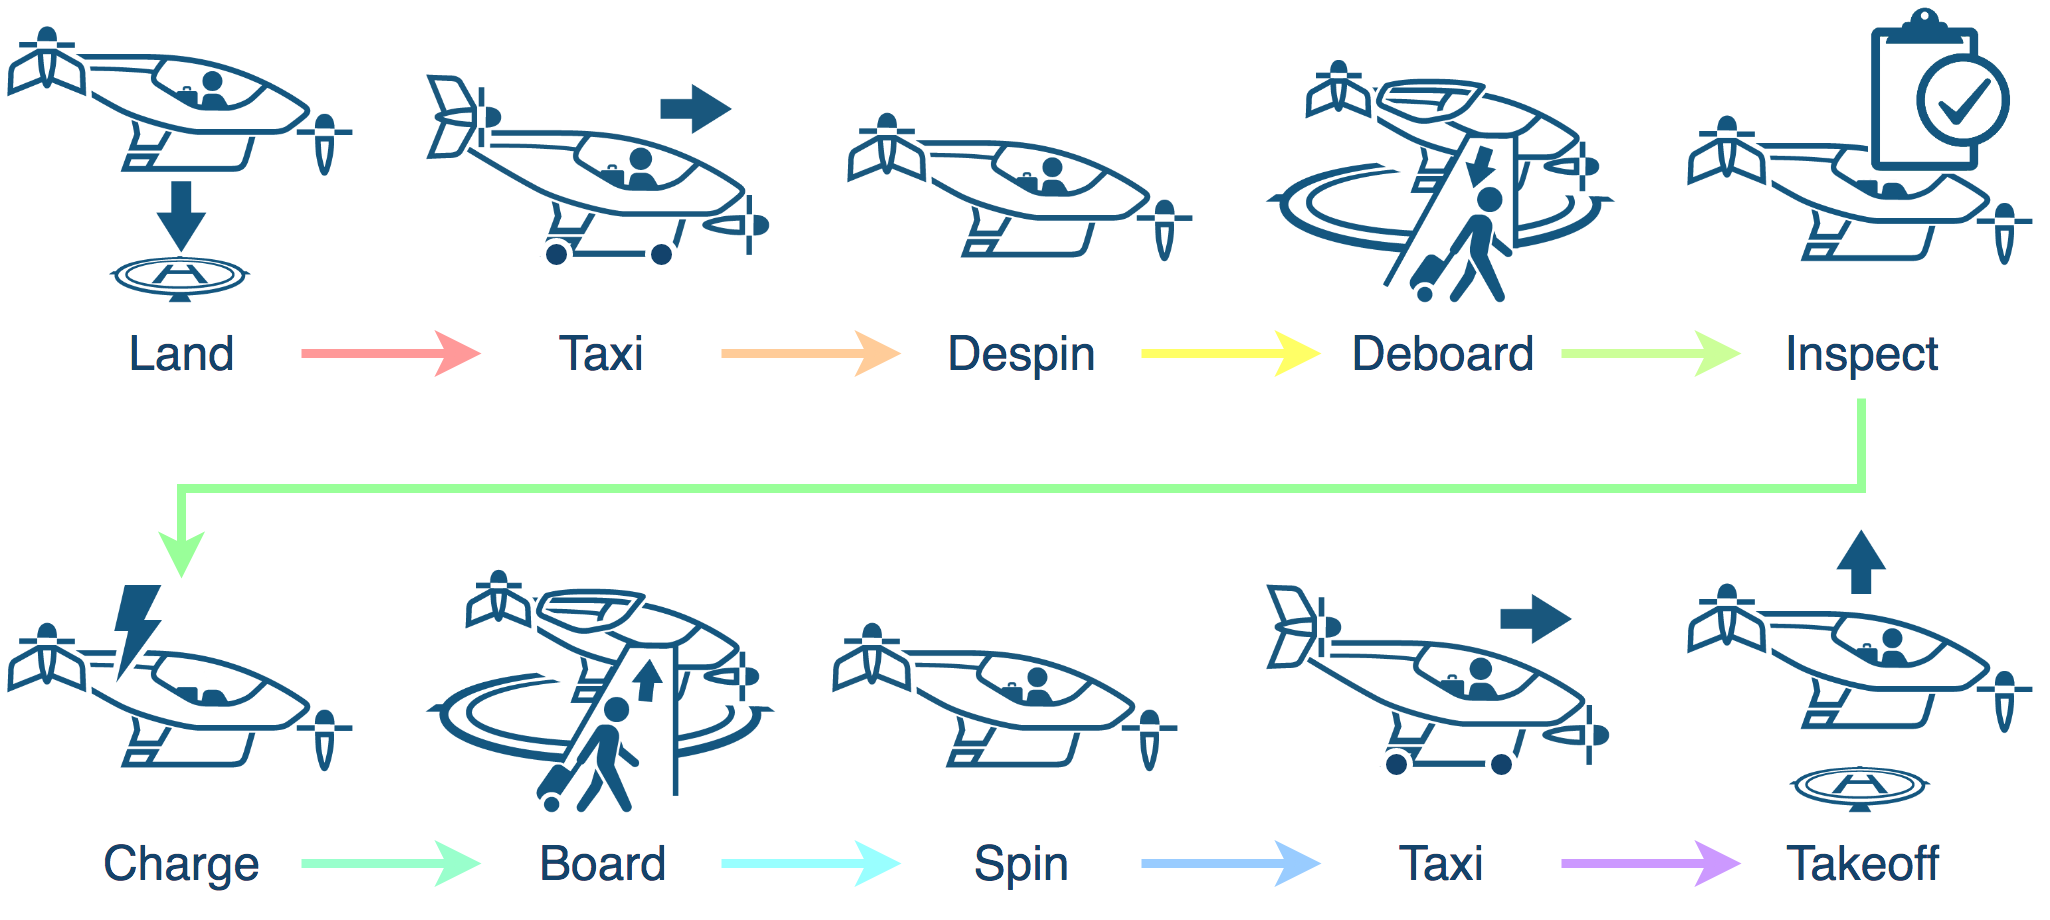
\includegraphics[width=0.6\textwidth]{Figures/journey-turnaround.png}
    \captionsetup{justification=centering}
    \caption{The "turnaround" time of a vehicle accounts for all time on the ground. Charging/refueling can occur concurrently with boarding and inspection.\protect\footnotemark}
    \label{fig:turnaround}
\end{figure}
\footnotetext{Icons courtesy of Vahana - \url{https://github.com/VahanaOpenSource/iconography} \url{https://vahana.aero/urban-air-mobility-iconography-5ad4de1fbca0}}
}

In the event that charging takes longer than boarding, this is a lower limit on the turnaround time.

\begin{equation}\label{eq:turnaround}
\begin{split}
    \underbrace{1.5}_\text{land}+\underbrace{1.5}_\text{taxi in}+\underbrace{0.5}_\text{despin}+\underbrace{0.5}_\text{spin}+\underbrace{1.5}_\text{taxi out}+\underbrace{0.5}_\text{takeoff} = 6 = t_\text{taxi} \\
    \underbrace{0.25\cdot n_\text{pax}}_\text{deboarding}+\underbrace{2}_\text{inspection}+\underbrace{0.5\cdot n_\text{pax}}_\text{boarding}+\underbrace{0}_\text{downtime}  = t_\text{boarding} \\
    t_\text{turnaround} = \text{max}\left( t_\text{boarding}, t_\text{charging}\right) + t_\text{taxi}
\end{split}
\end{equation}

Next, the journey time must be determined. This comes from a combination of the system design as well as the vehicle range and cruise speed. For the trade-off, multiple vehicle configurations are considered against three possible system configurations.

\paragraph{Centralized System}
% include image
In the centralized port arrangement, each vehicle flies a mission out from the vertiport to any location, and then back. In the ideal case, it carries a maximum load of customers in both directions. This means there are two flight cycles of takeoff, cruise and landing, plus an additional boarding sequence while away from the vertiport.
%(depicted in \autoref{fig:journey-central}. 
A single flight cycle can utilize the maximum range of the vehicle, and the "two-cycle" range (one way) can be easily calculated from \autoref{eq:twocycle}. The parameter $E_\text{TO}$ is a ratio specifying the percentage of the usable battery charge consumed for takeoff and ascent. For simplification, it is assumed the energy consumption for landing is the same as (or less than) cruise.

\begin{equation}\label{eq:twocycle}
    r_\text{2-cycle} = \frac{1}{2}r_\text{max}\frac{1 - 2\cdot E_\text{TO}}{1 - E_\text{TO}}
\end{equation}

% \begin{figure}[h]
%     \centering
%     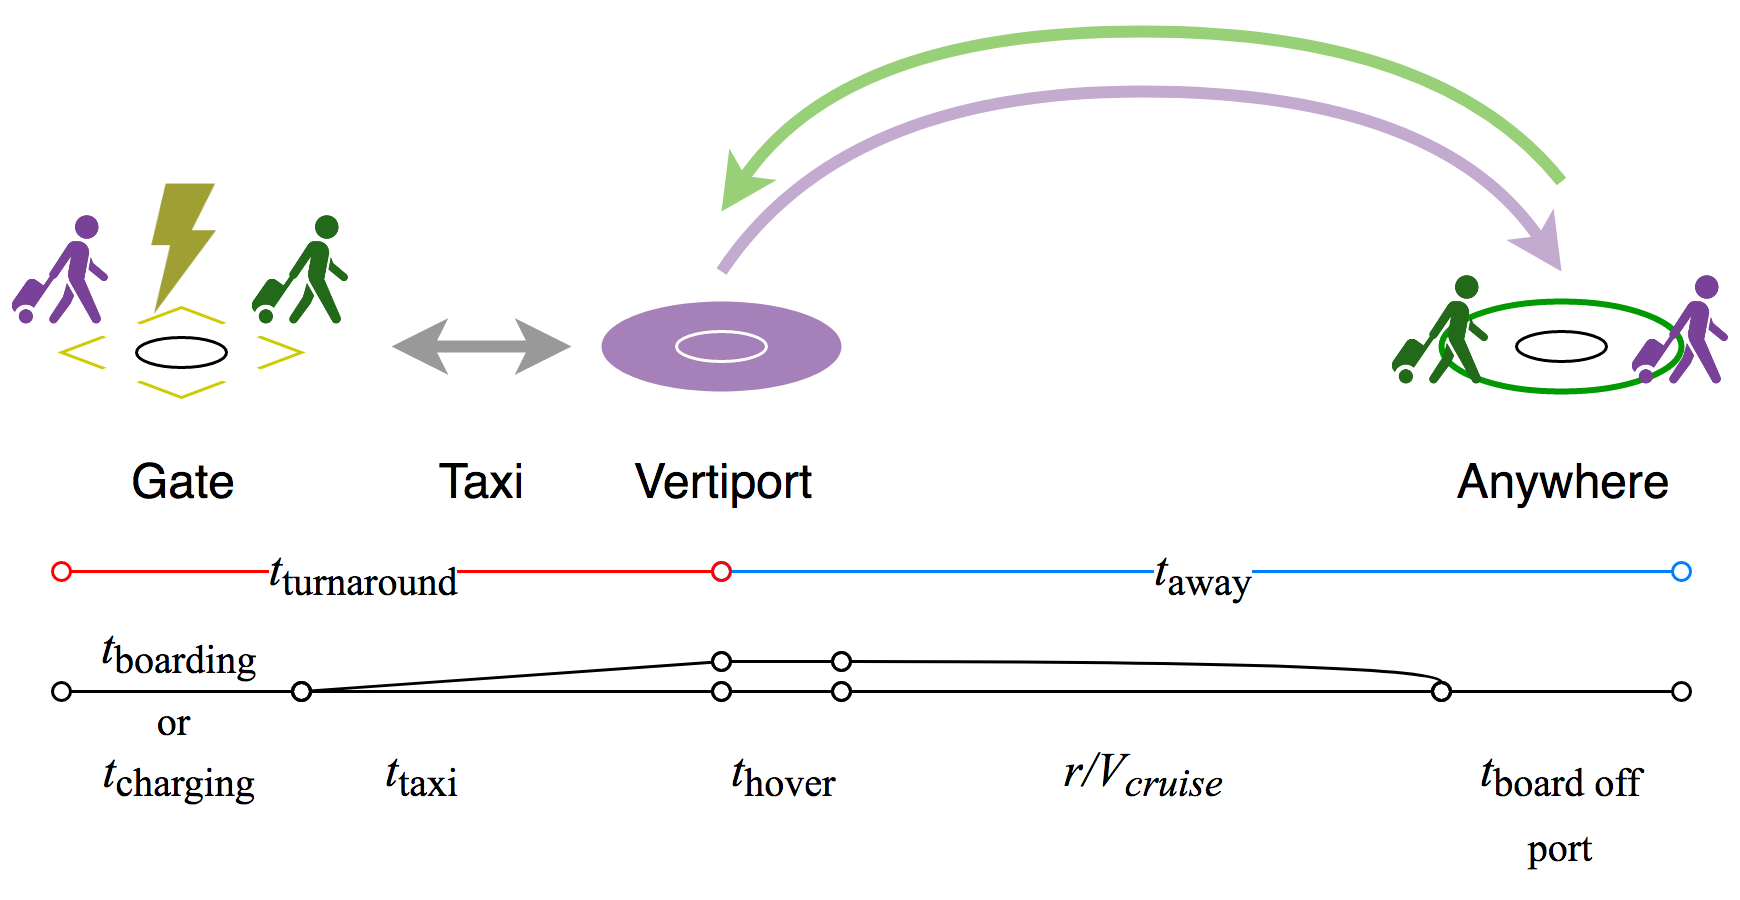
\includegraphics[width=0.8\textwidth]{Figures/journey-Central.png}
%     \captionsetup{justification=centering}
%     \caption{The "Centralized" system features the ability to drop-off and pick up customers anywhere. One endpoint of all journeys must be at a vertiport.}
%     \label{fig:journey-central}
% \end{figure}

The time that the vehicle is away from the vertiport ($t_\text{away}$) is simply a sum of the flight cycles and the boarding time (not at the port) plus a small amount of hover time ($t_\text{hover}=0.5$) that may occur when negotiating landing and takeoff.

\begin{equation}\label{eq:boardingOffport}
    t_\text{away} = \underbrace{1.5}_\text{land}+\underbrace{0.5}_\text{despin}+\underbrace{1\cdot n_\text{pax}}_\text{boarding} +\underbrace{0.5}_\text{spin}+\underbrace{0.5}_\text{takeoff} + 2\cdot r_\text{2-cycle}/V_\text{cruise} + 4\cdot t_\text{hover}
\end{equation}

From the time away and turnaround time, a \textit{gate capacity} is defined as $\frac{t_\text{away}}{t_\text{turnaround}} + 1$. This capacity represents the maximum number of vehicles that can be handled by a single gate. The \textit{gate throughput} can also be calculated as the number of vehicles served per hour. By multiplying this by the number of passengers, the number of passengers served per gate-hour can be determined. In the centralized case, it is multiplied by two, since there is a journey in and out of the gate, and no gate at the other end.

\paragraph{Port-to-Port System}
A port-to-port system limits the customer's journey end points to a vertiport location (depicted in \autoref{fig:journey-port}. This means that charging can occur after every journey. For the purpose of comparing to the centralized system, two cases are considered: where the journey length is the same as the centralized (using half the battery), and where the journey is the maximum range of the vehicle.

\begin{figure}[h]
    \centering
    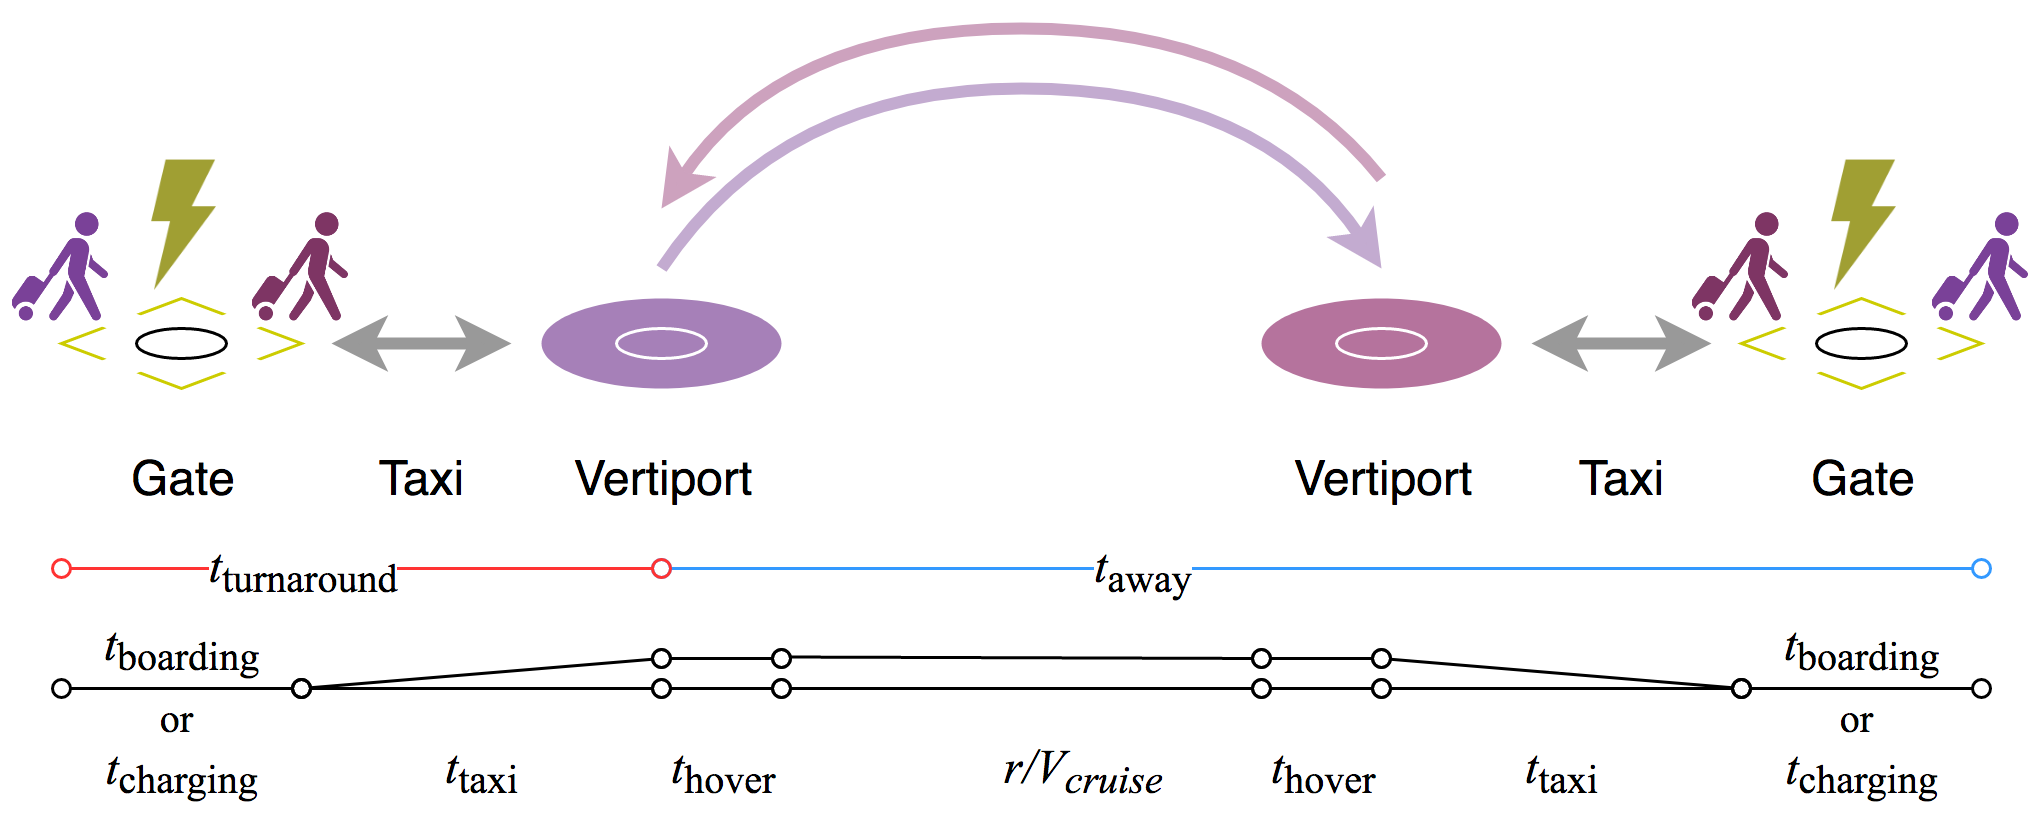
\includegraphics[width=0.8\textwidth]{Figures/journey-port-port.png}
    \captionsetup{justification=centering}
    \caption{When all customers travel vertiport to vertiport, the vehicle can charge after every flight. This diagram shows a complete cycle of two customer journeys.}
    \label{fig:journey-port}
\end{figure}

Some adjustments are made to the turnaround and away time calculations in each case. In the case where the journey length is the same, assuming no change to vehicle design, the battery charging time is half, possibly reducing the turnaround time. There is no boarding occurring away from a port, so the away time only accounts for the cruise and hover. Alternatively, it can be considered that the boarding and charging at the "other" port is part of the away time. Then, after determining the gate capacity, it must be divided by two, since there are two gates in the system.

\paragraph{Pure On-Demand System}
In a pure on-demand system, the vehicle will charge at a port where customers do not arrive or depart. The vehicle must fly two "zombie" legs of the journey to meet the customer and then drop them off, before returning to charge. This becomes a "three-cycle" trip.
% as depicted in \autoref{fig:journey-ondemand}. 
The length of each of the legs may vary, but the total range is still constant, assuming a constant amount of time used for hover and landing/takeoff. The total range of all three legs is calculated with \autoref{eq:threecycle}.

% \begin{figure}[H]
%     \centering
%     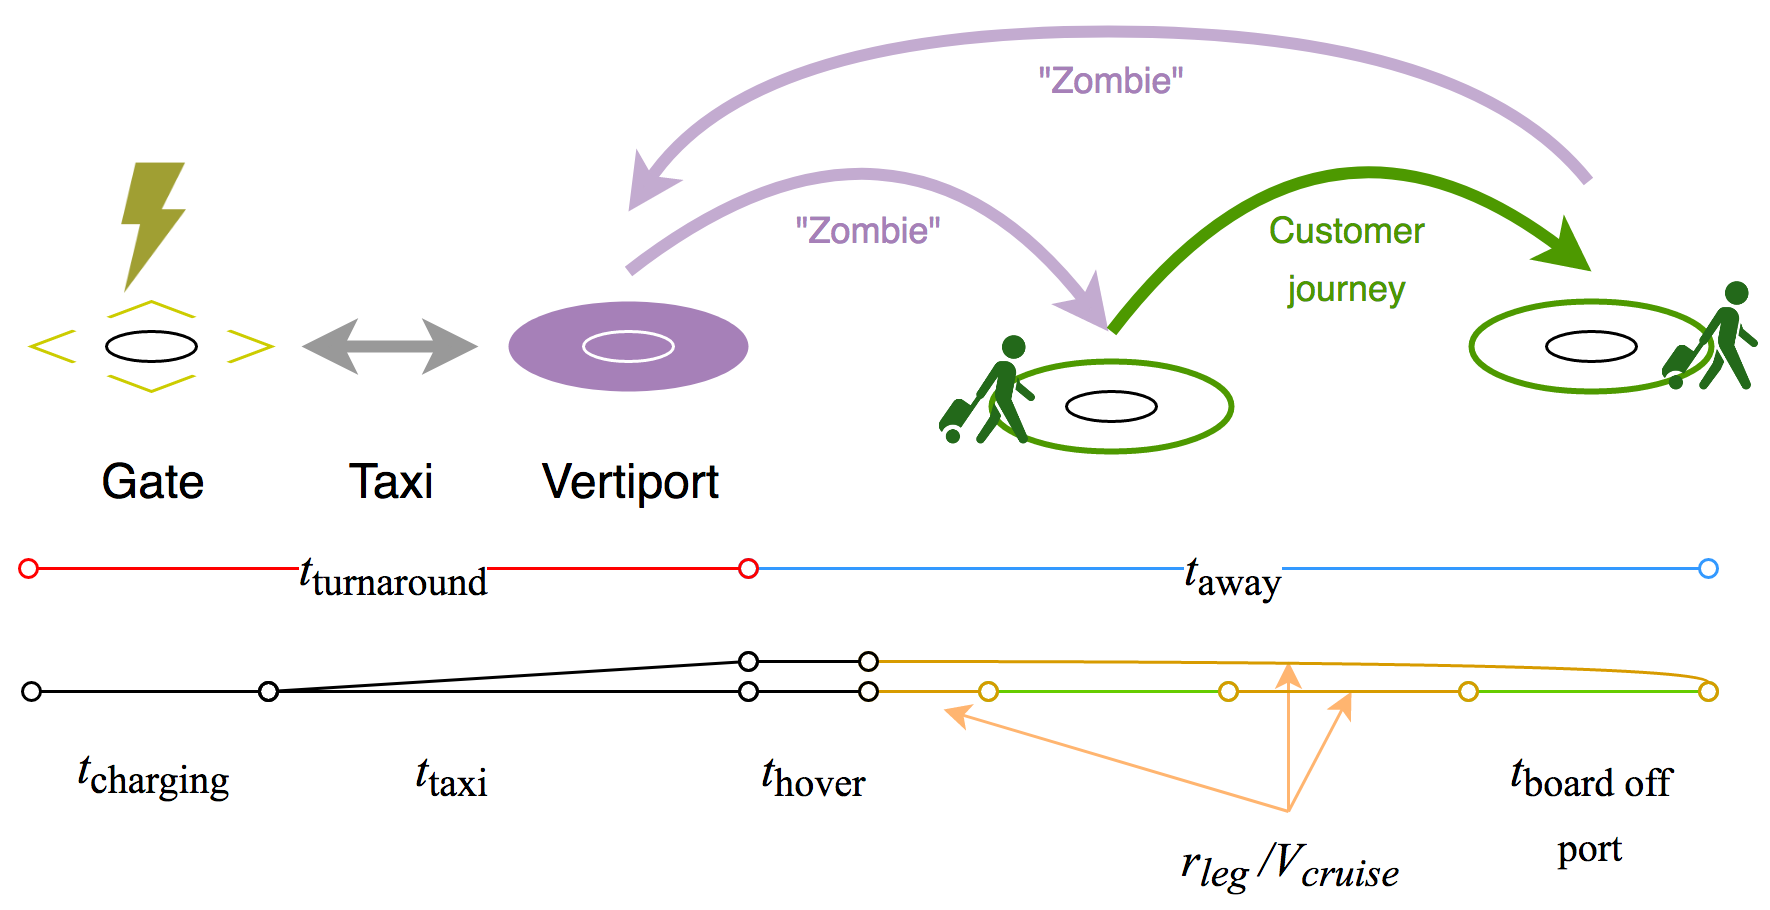
\includegraphics[width=0.8\textwidth]{Figures/journey-ondemand.png}
%     \captionsetup{justification=centering}
%     \caption{When all flights are on-demand, it is likely the vehicle will require up to two "zombie" trips to return to charge.}
%     \label{fig:journey-ondemand}
% \end{figure}

\begin{equation}
\label{eq:threecycle}
\begin{split}
    r_\text{total 3-cycle} = r_\text{max}\frac{1-3\cdot E_\text{TO}}{1 - E_\text{TO}}
\end{split}
\end{equation}

This system provides maximum customer options, but can be potentially wasteful in terms of energy used. To mitigate this issue, it is possible to shorten the "zombie" return trips if there are more available charging points throughout the system. Thus, vehicles can find the nearest charge point, and the customer portion of the journey could be a much higher percentage of the total range. In addition, the zombie trips use less energy per km. For the sake of the trade-off, the customer journey range is assumed to be on average half the total vehicle range. This assumes the maximum range in the case that the vehicle returns to the same charge point.















\subsection{Vertiport Design} \label{subsec:vportDesign}
As said in the introduction of this subsection the throughput of a vertiport is also limited by the vertiport design. There are different configurations for the vertiport design with specific benefits. The four different topologies are:
\begin{enumerate}
    \item \textbf{Linear Topology} A linear topology has many TLOF pads which increases the throughput. However, the throughput is restricted because it is not possible to have independent approaches and departures. Next to that, if the number of gates is limiting, the turnaround of a vehicle will increase, which means that the throughput of the vertiport will be lower. The linear topology will be mostly used when there is a thin long infrastructure available. In Los Angeles there is a pier topology on the Hooper Heliport.
    \item \textbf{Satellite Topology} The satellite topology is the most compact design of a vertiport with different TLOF pads and gates. The TLOF pads can be used independent for approaches and departures if the distance between the two pads is great enough. This topology can be implemented on rooftops.
    \item  \textbf{Pier topology} This topology is used for larger facilities. There are many TLOF pads and gates. This is the best configuration for vehicles with a longer turnaround time.
    \item \textbf{Remote apron topology} This topology has a TLOF pad located seperately of the gate. As a consequence the hovering/taxi time increases, however this topology supports simultaneous arrivals and departures on the TLOF pads.
\end{enumerate}
The combination of TLOF pads and gates is of great importance to increase the throughput. In a study the optimal gates with one TLOF pad is determined to be four or five to have the highest TLOF pad utilization\footnote{\url{https://pdfs.semanticscholar.org/243f/41d9ed601da27582f08d33426f80aa95f794.pdf}[accessed: 10-05-19]}. The design of a vertiport is determined by the dimensions of the vehicle. The tip-to-tip span of a vehicle determines the TLOF pads. Next to that, there are restrictions on the dimensions of vertiport designs. For the hover taxi and ground taxi route the minimum dimensions are 2 and 1.5 rotor diameters (tip-to-tip spans) of the design aircraft. In previous studies it has been concluded that ground taxi is recommended for a higher throughput. Moreover it is assumed that, "the gates have a diameter equal to the maximum vehicle dimension plus either 10 ft for ground taxi operations, or the greater of 10 ft or 1/3 rotor span for hover taxi operations\footnotemark[\value{footnote}]". A taxiroute may not come within 1/3 of the tip-to-span distance between the gates and taxiways. These restrictions will lead to complex design of the vertiport and should be optimized to create the highest throughput. In \autoref{fig:vertiport} the restricted dimensions are shown.

\begin{figure}[H]
    \centering
    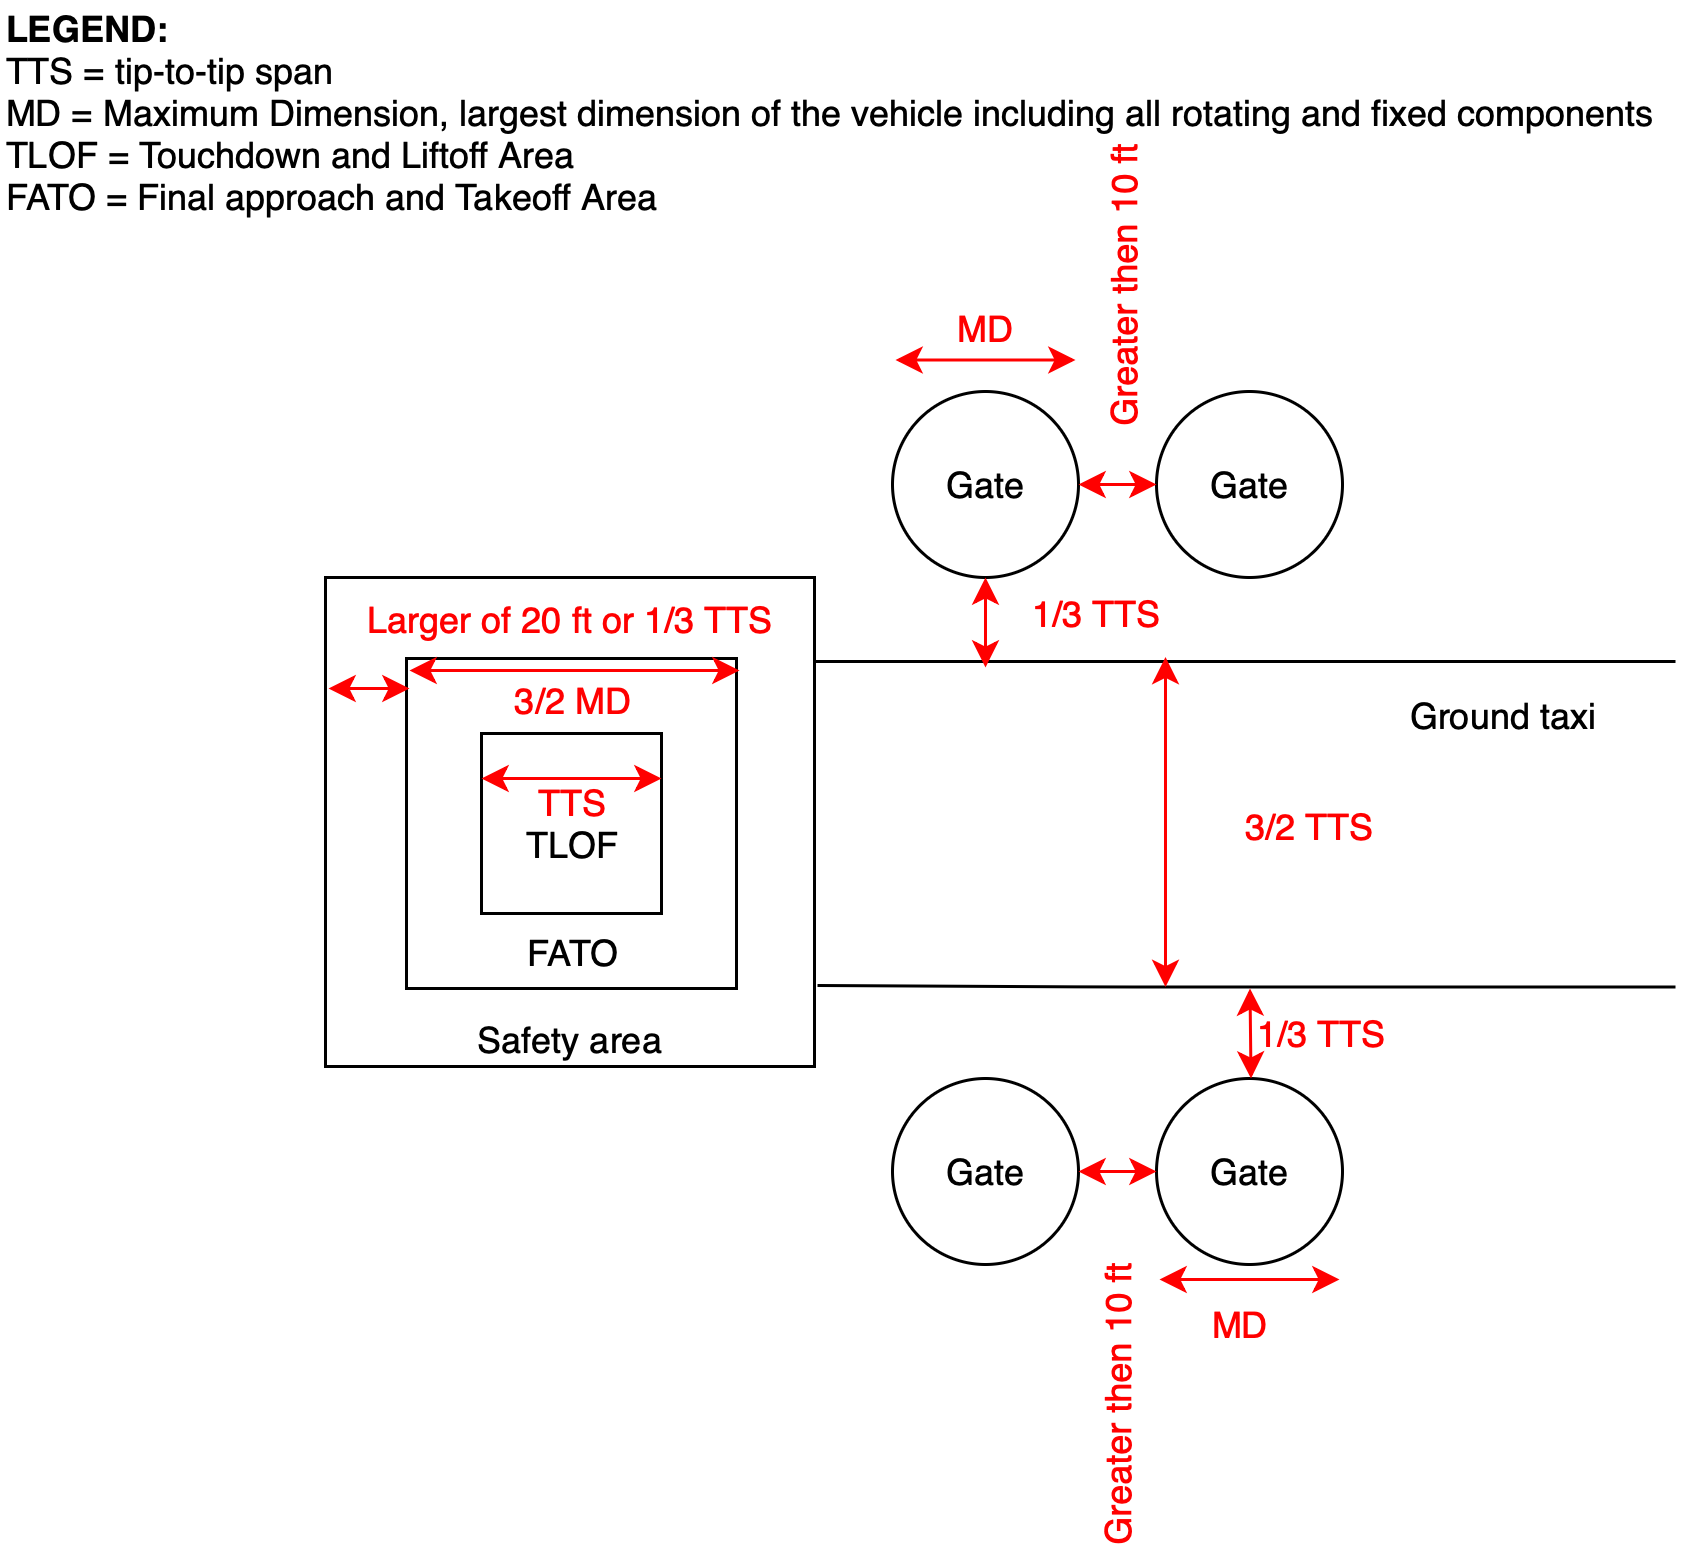
\includegraphics[width=0.5\textwidth]{Figures/Vertiport_design.png}
    \captionsetup{justification=centering}
    \caption{Vertiport design}
    \label{fig:vertiport}
\end{figure}









\subsection{Required ATC Efforts}
When measuring the air traffic control (ATC) efforts required for a given system, it is intended to measure two main factors: scalability challenges and service challenges of the ATC system \cite{ATC}. The scalability of a system refers to the ability to accommodate the throughput demand. In physical terms, it is equal to the amount of trips which a specific airspace management system can accommodate, while causing no more than a specified amount of trip delay. Barriers for a given system include the air traffic restrictions, air traffic density and the selected route design.
The service challenges of a ATC system relate to the complexity in operating the particular system. Challenges include the level of complexity in making traffic control decisions and the amount of staffing needed to manage the entire system with vehicles.

\paragraph{Tool Design}
In order to trade off the ATC efforts required for different systems, a qualitative tool is developed to measure ATC system characteristics that are indicative of the scalability and complexity of servicing the air traffic. The following ATC criteria are therefore evaluated: the air traffic density and the amount of interference of the given network design. \\

The air traffic density will be assessed via two sub-criteria: the maximum throughput flux obtained at the most congested hub, and the size of the vehicle. The throughput at the most congested hub measures the highest level of vehicle traffic density obtained through the system, which therefore evaluates the highest level of air traffic effort required. The size of the vehicle evaluates the complexity in accommodating a given number of vehicles in a restricted amount of airspace, due to separation restrictions and safety measures. It is therefore a measure of how much extra organisation and effort is needed to make the route network and flight scheduling feasible. The air traffic density values obtained may also pose some constraints on the total allowable amount of vehicles within the whole system and the maximum throughput at a hub, and therefore must be considered for different design options.
The level of interference is measured via a qualitative analysis of the physical location of the routes in parallel with the map of where potential interference are located. This criteria gives an overview of the level of potential air traffic interference with other entities using the airspace, which evaluates the level of air traffic management needed to accommodate the different entities' demands, and to minimise the probability of impacts. The type of potential interference will be separately assessed and are treated as sub-criteria. One type of intersection is the number of airport crossing the flight routes and the second type is the intersection between flight routes for a given route system. 

\paragraph{Criteria Weights}
In order to give appropriate importance to the particular criteria and sub-criteria used in evaluating the ATM efforts needed, a weighting factors are given. Weights are assigned by averaging the individual weights given to the criteria by each of the team members. The resultant weights are shown in \autoref{UAM-effort}: 

\begin{table}[H]
\captionsetup{justification=centering}
\caption{Weights of the various ATC effort criteria}
\label{UAM-effort}
\centering
\begin{tabular}{|l|l|l|l}
\cline{1-3}
\textbf{Criteria}  &     \textbf{Sub-criteria}   & \textbf{Weight}  \\ \cline{1-3}
\multirow{2}{*}{\textbf{Air Traffic Density}} & Vehicle Size  &  3.1  \\ \cline{2-3}
                                         & Maximum Hub throughput &  3.9 \\ \cline{1-3}
\multirow{2}{*}{\textbf{Level of Interference}} & Level of airport interference  & 3.5   \\ \cline{2-3}
                                         & MLevel of route intersections & 4.1  \\ \cline{1-3}

\end{tabular}

\end{table}















\subsection{Cost estimation}
The cost estimation for the system is an important aspect. For each system two types of costs are estimated, namely production costs and operational costs. Afterwards, these costs are combined and a break even point is determined. This is the point where the total costs are exactly the same as the incoming costs over a few years. If the break even point is known, the ticket price can be determined. 

The production costs of the system are based on the production cost per vehicle, the avionics costs per vehicle, battery costs per vehicle and the costs to build a hub. The total production costs is then the sum of the vehicle related costs multiplied with the fleet size and the costs to build a hub multiplied with the number of hubs that will be created. Moreover, the operational costs are dependent on the amount of trips per vehicle. These costs are determined by power, maintenance, infrastructural and ground costs. The costs for some of these aspects can be adjusted for each system. If you decrease the amount of hubs, the infrastructural costs will decrease. These parameters can all be adjusted for each system. However, the labour costs are set values per hour found from literature. Nevertheless, the number of employees might differ for each system. 

If the break even point is set on 15 years, the amount of trips made during those 15 years can be easily determined. This will be done by multiplying the trips served per day times the total days in a year (365 days) and then multiplied with the years. The operational costs will increase linearly over these years, because the amount of trips is assumed to increase continuously.

The revenue of the system is determined by the ticket price multiplied with the amount of trips. This will also be a linear relation as the number of trips increase linearly to the break-even point. A simple version of the outcomes can be seen in \autoref{fig:breakeven}.

\begin{figure}[H]
    \centering
    \captionsetup{justification=centering}
    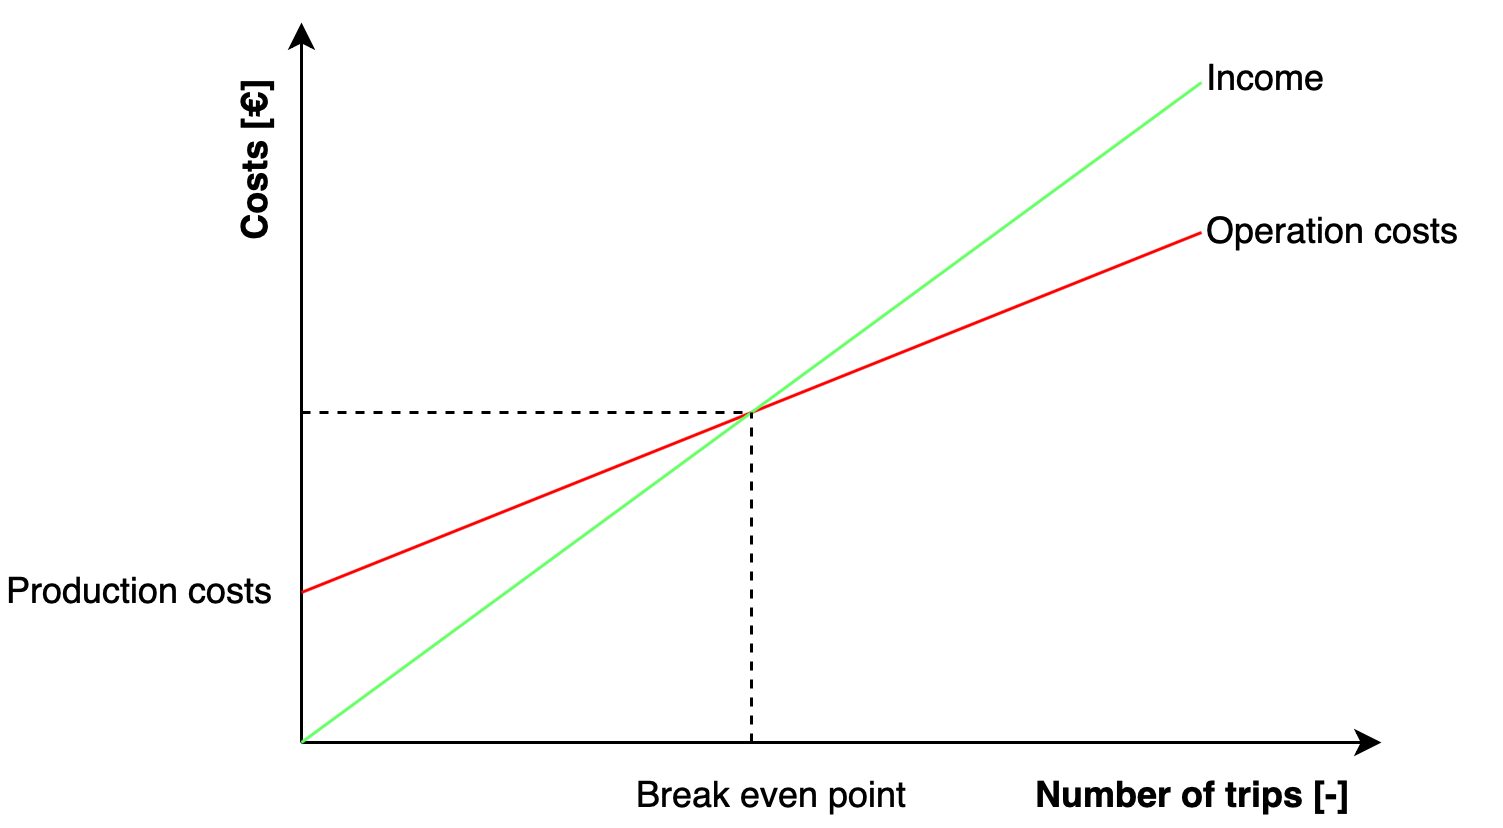
\includegraphics[width=0.8\textwidth]{Figures/Ticketprice.png}
    \captionsetup{justification=centering}
    \caption{Break even analysis}
    \label{fig:breakeven}
\end{figure}

The break-even point is set on a certain amount of trips. Based on this time aspect, the total costs and revenue can be set equal to each other. The ticket price per trip per vehicle can now be determined. To calculate the ticket price per passenger, the previous value is divided by the amount of passengers in the vehicle.

The development costs are not taken into account, because it is hard to quantify them for the three different systems. However, the technical readiness level for subsystems is taken into account. "Technology Readiness Levels (TRL) are a type of measurement system used to assess the maturity level of a particular technology" \footnote{\url{https://www.nasa.gov/directorates/heo/scan/engineering/technology/txt_accordion1.html}[accessed 13-05-19]}. There are 9 technical readiness levels, with TRL 1 as lowest level and TRL 9 as highest level. The weight, battery capacity and noise are subsystems that will be evaluated for the TRL. The total score of the technical readiness level will give a qualitative indication for the development costs. 

As mentioned above, it is hard to stick a number on the development costs at this stage in the design process. It is, however, possible to create an initial breakdown of these costs in terms of what percentage of the development cost budget they would roughly . The development costs consists of several parts. Firstly there is the 'Project Management' which contains the costs of the labourers and contractors. Next there are the costs for the hardware and software, which include things servers or the costs that are made for the licences and the development of the software. There is the testing, which is likely a function of how much hardware and software there is. Lastly there are the costs that have to be made to train the personnel and for other supporting activities. An initial indication of how much of development costs each of the aforementioned categories take up is presented in the table below \ref{Devcosts}. 



% Please add the following required packages to your document preamble:
% \usepackage{booktabs}
\begin{table}[H]
\centering
\captionsetup{justification=centering}
\caption{Breakdown of development costs}
\label{Devcosts}
\begin{tabular}{@{}ll@{}}
Category            & \% of Development costs \\ \midrule
Project Management  & 20                      \\
Hardware            & 5                       \\
Software            & 40                      \\
Testing             & 15                      \\
Training \& Support & 15                      \\
Reserves            & 15                      \\ \bottomrule
\end{tabular}
\end{table}







\section{Tool integration} 
\label{sec:toolintegration}

After creating the tools presented above, they somehow needed to be integrated together so as to produce one umbrella tool (hereafter referred to as the tool) that any user could use easily. A flowchart of the tool can be found in the fold-out page below. 

The input of the tool consists of variable and fixed parameters, which can be grouped in \textit{Atmospheric}, \textit{Vehicle} or \textit{Operational} parameters. The \textit{fixed} parameters will never be changed by the user and include all atmospheric parameters, cruise altitude, total time savings provided to the customers, break-even point, observer location, etc (see green diamond-shaped blocks in the flowchart). The \textit{variable} parameters are the parameters that depend on the inputs of the user. Since the user in this case is someone who wants to evaluate a concept design, he/she will have the freedom to change most vehicle \& operational parameters. Examples of \textit{specifiable vehicle parameters} are number of passengers, the type of propulsion units used by the device, the vehicle configuration, the vehicle maximum dimension the type of battery, etc. Depending on the vehicle configuration chosen, the MTOW, range, cruise velocity and structural mass percentage (everything excluding payload and batteries) will be inputs of the user, as shown in the flowchart.  Examples of \textit{specifiable operational parameters} are the number of routes to serve, the minimum trip distance to serve, etc.

%Here goes the flowchart and an explanation of how the whole pipeline works from start to finish (basically a guide on how to use the tool). DAVID in charge


The user will specify the parameters of the design vector (vehicle and operational parameters) in \newline \texttt{defineConcepts.m}. These parameters will be assigned to MATLAB objects which are instantiated in the main script, \texttt{main.m}. After instantiating the Atmosphere, Vehicle, and Operational objects, \texttt{main.m} will execute one of three options, depending on the vehicle configuration chosen:

\begin{enumerate}
    \item \texttt{veh.config = "reference"}: A reference vehicle is being put into the tool, for which the MTOW, range, cruise velocity (and hopefully the type of battery) are known. The tool will then proceed by calculating the structural percentage needed for the vehicle to fly the specified mission with the batteries chosen. It will also return the rest of outputs of the tool, such as noise, ticket price, etc, which can be used as a baseline.
    \item \texttt{veh.config = "outlier"}: this configuration can be used either when the vehicle being input is very novel or when sensitivities around a reference vehicle are to be computed. In case of the former, a structural percentage, range, and cruise velocity have to be estimated, and the tool will calculate the MTOW needed to fly the mission. Some trial and error might be necessary to find what mission the vehicle in question is suited for. In case sensitivities are to be computed, the structural percentage calculated in the run \texttt{veh.config = "reference"} is specified, along with a modified cruise speed, range, or any other parameter, and a new MTOW will be computed.
    \item \texttt{veh.config = "tilt"/"multi"/"fixed"/"avg"}: whenever your vehicle looks similar enough to an existing tilt-wing, multi rotor, fixed-wing vehicle (or a mix) that the user prefers to rely on statistics to estimate the range, cruise speed and MTOW of the vehicle. The user will specify only the number of passengers to obtain these parameters. L/D$_{\text{cruise}}$, the battery type and the propulsion units specified for the vehicle will be used to calculate the battery mass needed and the resulting structural percentage.
    
\end{enumerate}


Once the Vehicle and Operations objects have been updated, they can be used to calculate the top N trips where the  system will provide the largest G, defined in \autoref{eq:gainmetric}. Subsequently, with the M unique route lengths in the N trips chosen, an air time and a turnaround time will be calculated (both a function of trip distance, assuming charging happens after every trip to full charge). These times will be used to calculate the fleet size, the energy needed to operate these vehicles per day and the total battery mass of the fleet. Once the fleet size, the air time and turnaround time are known per route, the number of gates per hub can be calculated. From there, the number of landing pads can be calculated using the optimal ratio of 4 gates per landing pad. This is under the assumption that the number of gates is limiting and not the number of pads. The number of pads would be limiting if the number of landings and take-offs divided by the previously found number of landing pads causes the vehicles to travel too close to each other.

Knowing the fleet size and the battery mass in every vehicle, a simple multiplication leads to the total battery mass used by the system (note that life cycle of batteries has not been considered at this stage). By knowing the number of landing pads needed and the maximum size of the vehicle, the total ground footprint of the system can be calculated. 

The total costs for production and operation of the system (including the hubs) up to the BEP, together with the number of passengers transported will be used to estimate a ticket price/pax/km.

A calculation that also emerges from the Vehicle and Operational updated objects is the calculation of noise and downwash. The calculation of these figures is done in hover, and is heavily dependent on the thrust distribution across the different rotors in the vehicle. For modularity purposes, the function \texttt{defineConcepts.m} allows the user to specify different Propulsion Units (PUs). PUs consist of a set of rotors that have the same design parameters and operate in the same conditions. Key parameters to specify for each propulsion unit are the number of rotors in that propulsion unit, whether the rotors are operated in hover, cruise or both, the rotor configuration (single or coaxial) and the thrust that the unit provides in hover/total thrust. These parameters will be key drivers in the calculation of noise and downwash, which is computed for each PU separately and then summed across in an appropriate fashion. For instance, in the total noise computation, decibel arithmetic is used and no destructive interference between sources is assumed (which is valid if the sound source is emitted at different frequencies). In the downwash computation, a weighted average is calculated to find the downwash velocity of the device. It seemed reasonable to weigh the velocity of each propulsion unit by the air mass flow going through each.


%on the vehicle configuration chosen load the database of trips


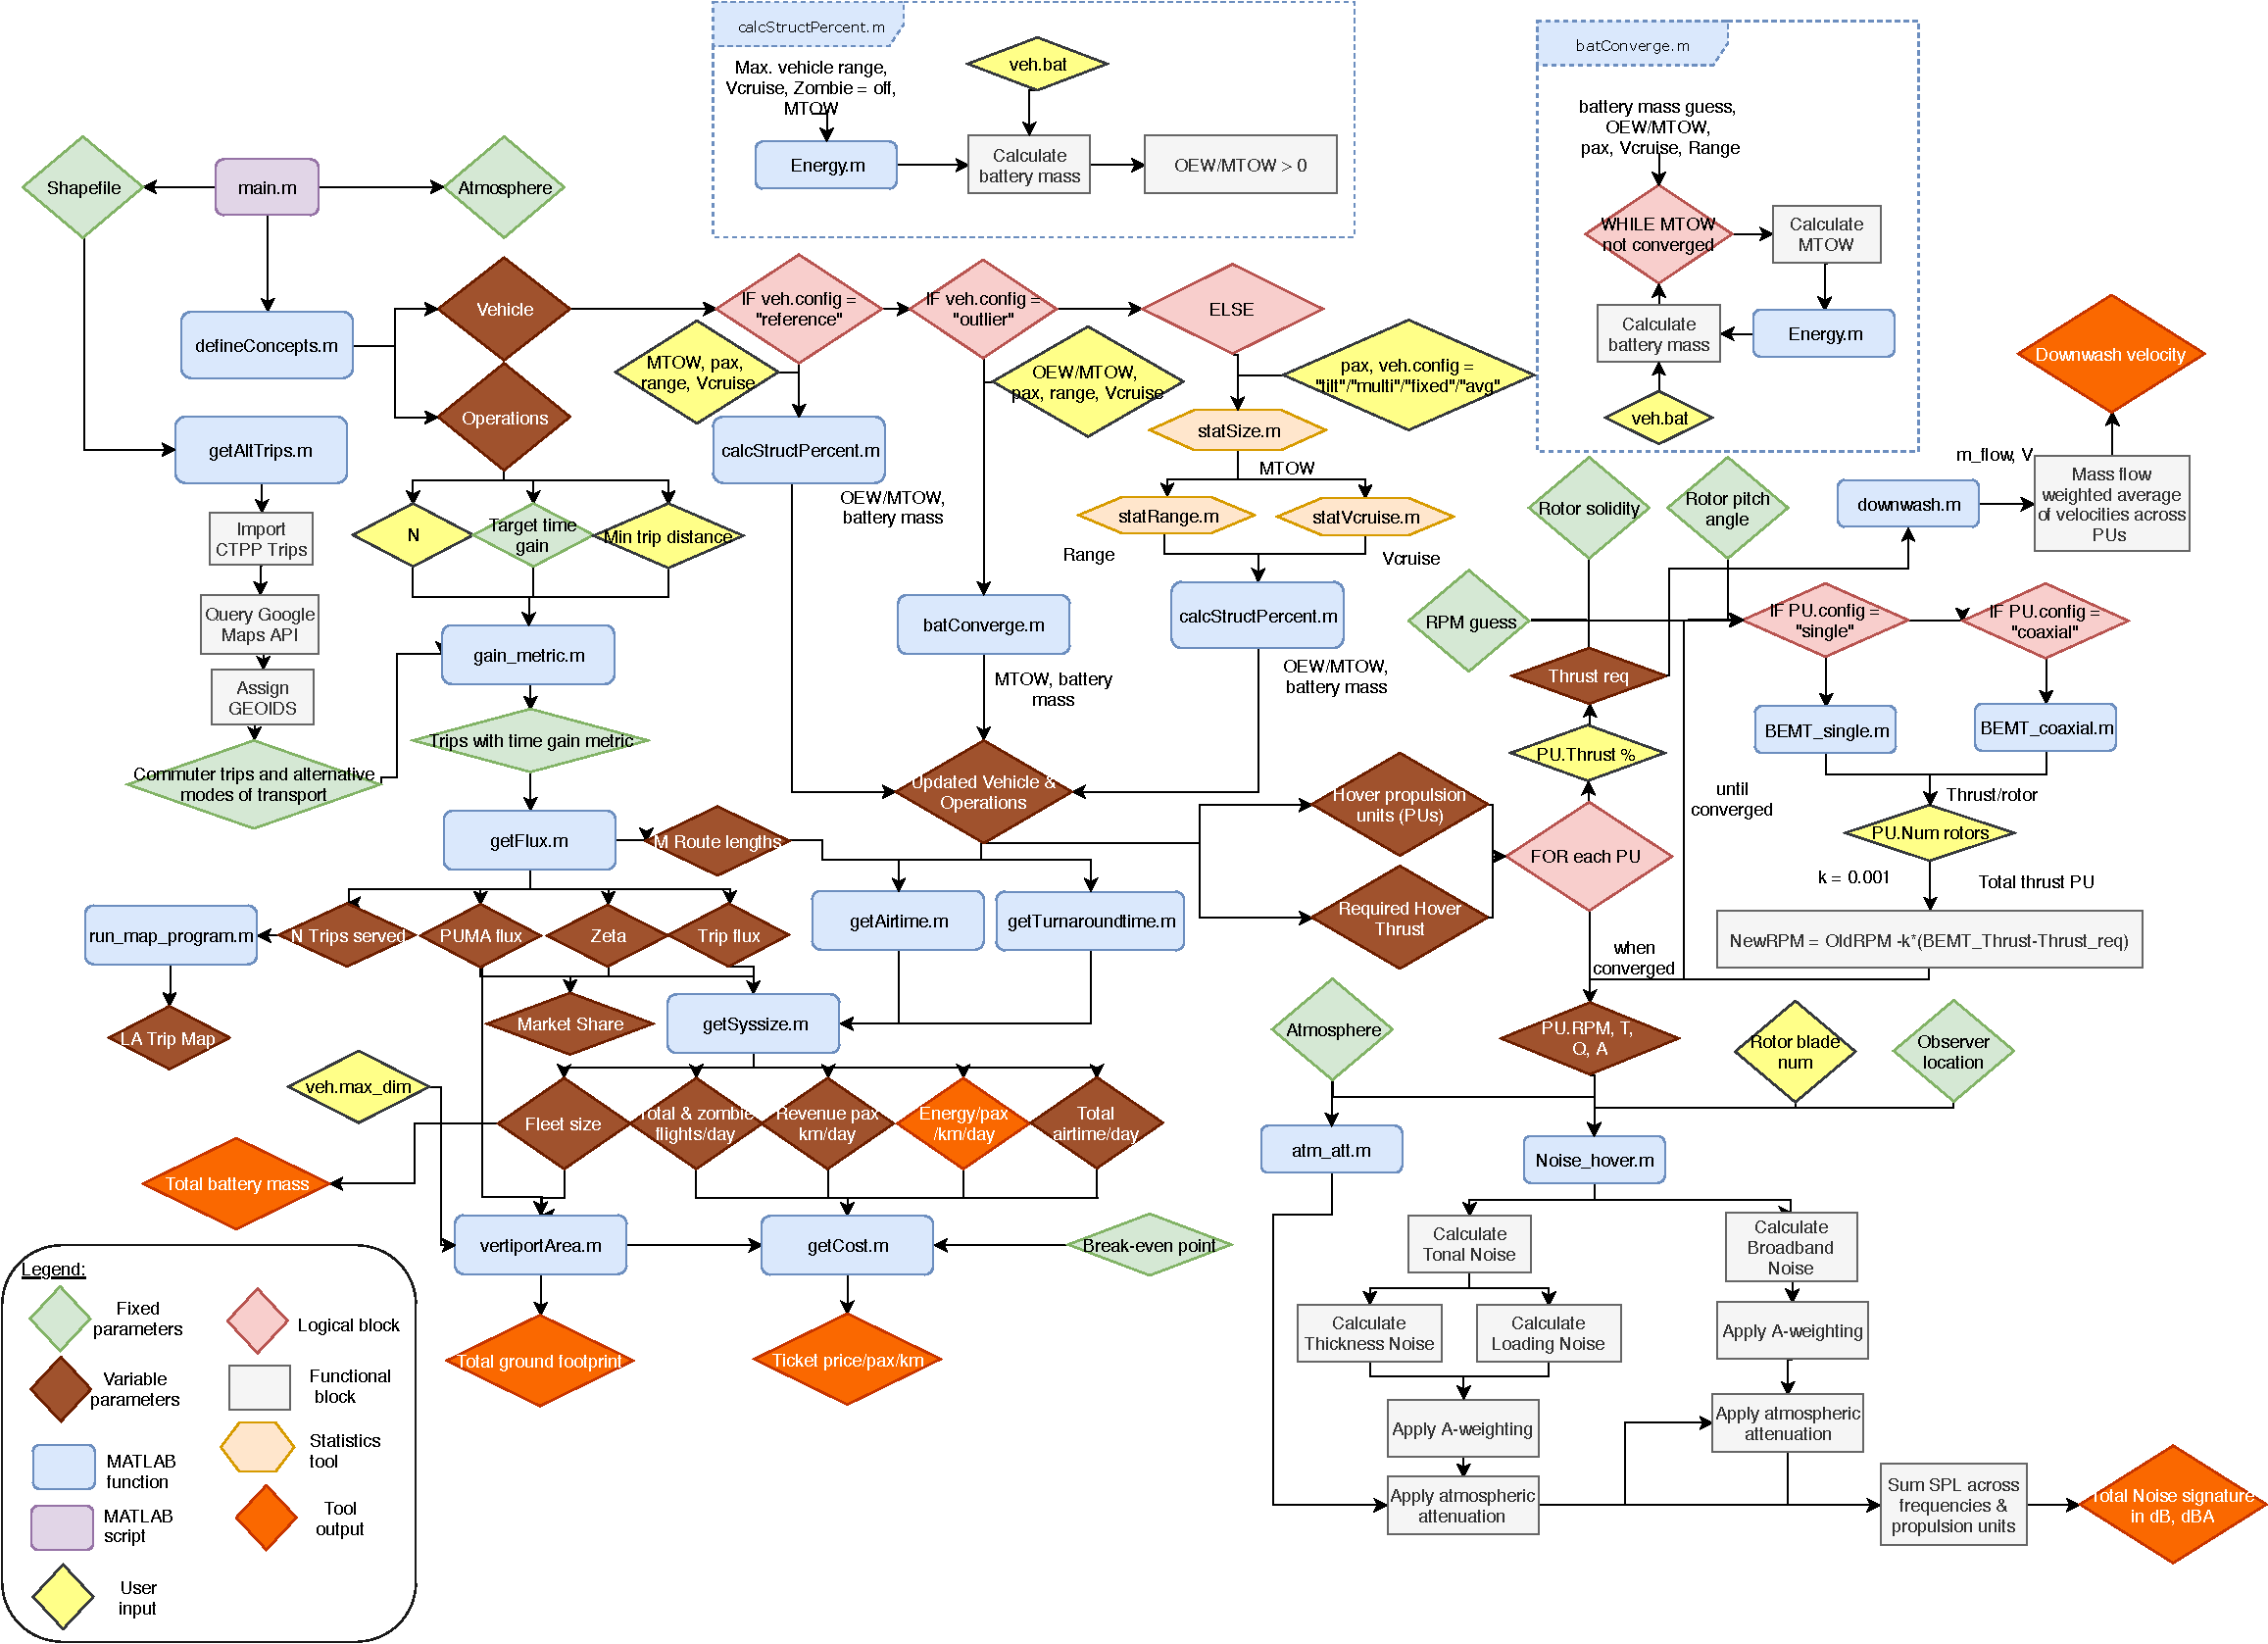
\includepdf[pages={1},fitpaper]{Figures/tool_flowchart.pdf}



\section{Sensitivity Analysis} 
\label{sec:sensitivityanalysis}

Evaluating one vehicle and operations concept design at a time quickly and with concise and reliable outputs is useful, but usefulness of the tool integration can be significantly enhanced by scripting a way of quickly exploring small design changes around a certain design and evaluating the changes in certain tool outputs of vehicle traits. This is known as sensitivity analysis and aids in trade-offs and risk assessment, because it can show how significant an uncertainty in a design parameter is on the overall system performance.

\subsection{Workflow Design}

The user sets $m$ input concepts and a list of $n$ inputs variables REFERENCE HERE to be perturbed within specified ranges and a list of $o$ outputs to be measured. The script evaluates all perturbations to the concepts and returns $o$ output files showing the relative change in the output parameters in $n$ plots (one for each perturbed input). Each plot contains $m$ lines; one for each concept.

The plots can be output using percentage changes for perturbation variables and/or output parameters or using the actual magnitudes or the metrics. Non-convergence of MTOW or BEMT for a certain input is treated as NaNs and those parts of the lines are not plotted.


\subsection{Applications}

If every variable is queried with a range of $p$ values, the analysis takes $(n+1)\cdot m\cdot p$ function evaluations, of which each takes roughly a full second. A broad sensitivity analysis was performed on $m=3$ remaining concept after the initial selection, with results shown in chapter \ref{ch:sensitivity}.

This tool was also used to perform a risk assessment of a set of assumptions made when writing the tools by multiplying the earliest output of a subtool affected by the assumption in question by a factor close to but different from one and then plotting the percentage changes of relevant outputs. If the change in the output is small, then the effect of a discrepancy in the subtool is less severe. However, if the change in the outputs is significant, more effort should be allocated to increasing confidence in the method or assumptions used, since small deviations already influence the final results.





 